% !TEX encoding = UTF-8 Unicode
% !TEX encoding = UTF-8 Unicode
\documentclass[UKenglish]{ifimaster}  %% ... or USenglish or norsk or nynorsk
\usepackage[latin1]{inputenc}        %% ... or utf8 or applemac
\usepackage[T1]{fontenc,url}
\urlstyle{sf}
\usepackage{babel,textcomp,csquotes,ifimasterforside,varioref,graphicx,caption,nameref,caption}
\usepackage[section]{placeins}
\usepackage{amsmath,lipsum}
\setcounter{secnumdepth}{3}
\interfootnotelinepenalty=10000
\usepackage{listings}
\usepackage{color}
\usepackage{array, dcolumn, booktabs,enumitem}
\usepackage[showframe=false]{geometry}
\usepackage{changepage}
\usepackage{subfigure}
\let\Chaptermark\chaptermark
\def\chaptermark#1{\def\Chaptername{#1}\Chaptermark{#1}}
\let\Sectionmark\sectionmark
\makeatother\newcommand{\mypm}{\mathbin{\smash{%
\raisebox{0.35ex}{%
            $\underset{\raisebox{0.5ex}{$\smash -$}}{\smash+}$%
            }%
        }%
    }%
}

\setlength{\parskip}{\baselineskip}%
\setlength{\parindent}{0pt}%

\definecolor{mygreen}{rgb}{0,0.6,0}
\definecolor{mygray}{rgb}{0.5,0.5,0.5}
\definecolor{mymauve}{rgb}{0.58,0,0.82}
\lstset{ %
  backgroundcolor=\color{white},   % choose the background color; you must add \usepackage{color} or \usepackage{xcolor}
  basicstyle=\footnotesize,        % the size of the fonts that are used for the code
  breakatwhitespace=false,         % sets if automatic breaks should only happen at whitespace
  breaklines=true,                 % sets automatic line breaking
  captionpos=b,                    % sets the caption-position to bottom
  commentstyle=\color{mygreen},    % comment style
  deletekeywords={...},            % if you want to delete keywords from the given language
  escapeinside={\%*}{*)},          % if you want to add LaTeX within your code
  extendedchars=true,              % lets you use non-ASCII characters; for 8-bits encodings only, does not work with UTF-8
  frame=single,                    % adds a frame around the code
  keepspaces=true,                 % keeps spaces in text, useful for keeping indentation of code (possibly needs columns=flexible)
  keywordstyle=\color{blue},       % keyword style
  language=Java,                 % the language of the code
  morekeywords={*,...},            % if you want to add more keywords to the set
  numbers=left,                    % where to put the line-numbers; possible values are (none, left, right)
  numbersep=5pt,                   % how far the line-numbers are from the code
  rulecolor=\color{blue},         % if not set, the frame-color may be changed on line-breaks within not-black text (e.g. comments (green here))
  showspaces=false,                % show spaces everywhere adding particular underscores; it overrides 'showstringspaces'
  showstringspaces=false,          % underline spaces within strings only
  showtabs=false,                  % show tabs within strings adding particular underscores
  stepnumber=1,                    % the step between two line-numbers. If it's 1, each line will be numbered
  stringstyle=\color{mymauve},     % string literal style
  tabsize=2,                       % sets default tabsize to 2 spaces
  title=\lstname,                   % show the filename of files included with \lstinputlisting; also try caption instead of title
  numberstyle=\tiny,
}








\title{Does Limit on Work-In-Progress (WIP) matter?}        %% ... or whatever
\author{Truls Skeie}                      %% ... or whoever 
\usepackage[
    backend=biber,
    style=authoryear-icomp,
    sortlocale=de_DE,
    natbib=true,
    url=false, 
    doi=true,
    eprint=false,
    citestyle=authoryear
]{biblatex}
% !BIB TS-program = biber

\addbibresource{lib.bib}

\begin{document}
\ififorside{}
\frontmatter{}
\maketitle{}

\chapter*{Abstract}                   %% ... or Sammendrag or Samandrag

\tableofcontents{}
\listoffigures{}
\listoftables{}
\lstlistoflistings{}

\chapter*{Preface}                    %% ... or Forord

\mainmatter{}
\chapter{Introduction}
\label{chap:intro}
In this master thesis the focus will be on limit Work In Progress (WIP) who is one of the principles in Kanban. The focus will be to see what impact WIP limit have in a development process. In order to do so, a data set gathered by an in house software company in Norway called Software Innovation (SI) is used. SI is a Scandinavian software company that delivers Enterprise Content Management applications. 

The data set has already been interpreted by another study. That study investigated Scrum vs. Kanban for SI. For interested readers the case study can be found in the article "Quantifying the Effect of Using Kanban versus Scrum: A Case Study" \parencite{Dag}. 

\section{Motivation}
In software development the processes and methods are important in order to deliver the right product on time. In software development one rarely solve two identical problems for different stakeholders. And the problems are getting bigger and more complex, which means that new processes and methods are introduced and the already existing processes and methods needs to adapt to solve the complex problems in the most efficient ways.  The number of popular software development methods  (e.g. Extreme programming, Spiral, Scrum and Kanban) emerged in the recent years proves the assumption \parencite{gandomani2013important} \parencite{ikonen2010exploring}.

This is why this thesis will focus on software development methods, the method in each development project is such a key element. Within software development methods, the main focus of this thesis will be the Kanban method and the principle to limit Work In Progress (WIP). In Kanban the WIP limit is used to  limit the number of tasks each developer can work on at each workflow state to prevent bottlenecks and to ensure flow of tasks through the development cycle \parencite{gandomani2013important} \parencite{ikonen2010exploring}.

There are published various literature on Kanban in software development such as "Kanban: Successful Evolutionary Change for Your Technology Business" \parencite{0984521402}, "Kanban and Scrum - making the most of both"  \parencite{Kniberg} and "Lean Software Management: BBC Worldwide Case Study" \parencite{Joyce}. Although there is various literature, there is no information on how to apply WIP limit, even though most of the experience Kanban enthusiasts agree that WIP limit is an important principle.  There is no research backing the statement.  The literature states that one should experiment with WIP limits in order to find the best WIP limit for one's case \parencite{Ikonen} \parencite{Kniberg}.

Since there is lack of available research on WIP limit my motivation is to investigate WIP limit in this thesis.

\section{Research Question}
\label{chap:RQ}
In this thesis the overall research question will be to study the effects of WIP limits for an in house software company, and to see if the research will give answers to the following question:
\begin{itemize}
\item Do WIP limit in software development matter?
%\item See if the exist an optimal WIP limit for a given context.
\item How to best find the optimal WIP limit?
\item Which parameters to consider in order to optimize WIP? 
\end{itemize}


\section{Approach}
This thesis will use case study as an approach in order to answer the research questions. To conduct the case study a data set from an in house software company will be used.  The data set will be calculated and analyzed. The first part of the analyze will be done by a program. The program was made for this thesis in order to calculate the data set. The program will turn the data set from quantitative into more suited quantitative data set. 

The analyzed data will be evaluated on team level. The most valuable teams will be picked and their data will be extracted form the data set by the program.  The most valuable teams will be picked on the basis of number of task labeled with their name in the data set.  After the program has calculated the most valuable teams, statistical analysis will be used to compute correlation and descriptive statistic.

The correlation and  descriptive statistic will be represented in chapter \ref{ch:res}. 
\section{Contribution}
My contribution to the research on WIP and WIP limit consist of creating a Java-based program that will measure WIP for each day based on a data set. For the program to work, the data set given as a parameter to needs to have the same format as the data set in this thesis. 

\section{Chapter overview}
\begin{description}
\item[Chapter \ref{chap:intro}: \nameref{chap:intro}:] \hfill \\
The first chapter will consist of a section where the motivation behind this thesis is stated. A section where the research questions this is stated. A section which gives a brief description of how I will approach the data set in order to answer the research questions and a section where my contribution to the research of WIP limit will be stated.
\item[Chapter \ref{chap:Background}: \nameref{chap:Background}:] \hfill \\  
Chapter \ref{chap:Background} consist of background information which gives a brief introduction to concepts and methods in software development as well as information about the in house software company, Software Innovation. These methods and concepts are referred to later in the thesis.  
\item[Chapter \ref{chap:RM}: \nameref{chap:RM}:] \hfill \\  
Chapter \ref{chap:RM} introduces and explains the research methods used in the thesis as well as complementary information about Software Innovation and why the data set from Software Innovation is used in this thesis.  
\item[Chapter \ref{ch:DCC}: \nameref{ch:DCC}:] \hfill \\
Chapter \ref{ch:DCC} gives information about the data set and the calculations. Complementary information about how the program operates is given in the chapter as well as information about how the output data from the program is measured using statistical analysis. 

\item[Chapter \ref{ch:res}: \nameref{ch:res}:] \hfill \\
\item[Chapter \ref{ch:dis}: \nameref{ch:dis}:] \hfill \\
\item[Chapter \ref{ch:con}: \nameref{ch:con}:] \hfill \\
\end{description}




%\textbf{Chapter \ref{chap:intro}: \Chaptername:} The first chapter will consist of a section where the motivation behind this thesis is stated. A section where the research questions this thesis will address. A section how I will approach the data in order to answer the research questions.  A section that will explain how I will evaluate the data in order to answer the research question and a section where contribution will be stated.   

\chapter{Background}  
\label{chap:Background}                %% ... or Bakgrunn
In this chapter there will be a brief introduction to Waterfall (Section \ref{sec:WP}), Scrum (Section \ref{sec:Scrum}), Lean (Section \ref{sec:Lean}) and Kanban (Section \ref{sec:Kan}) with affiliated tools. There will also be given a brief introduction to the software development company Software Innovation (Section \ref{sec:SI})

\section {Waterfall}
\label{sec:WP}
"The waterfall model is the classical model of software engineering. This model is one of the oldest models and is widely used in government projects and in many major companies" \parencite{munassar2010comparison}.

The main goal of the waterfall model is to plan in early stages to ensure design flaws before coding is started. Since planning is so critical in the waterfall method it fits project where quality control is a major concern  \parencite{munassar2010comparison}.

The waterfall method consist of several non-overlapping stages as shown in figure \ref{fig:waterfall}. The figure is an example of the waterfall model with a life cycle of establishing system requirements and software requirements and continues with architectural design, detailed design, coding, testing and maintenance  \parencite{munassar2010comparison}.

One of the main principles of the waterfall method discourage return to an earlier phase. For example returning from detailed design to architectural design. However, if returning to an earlier phase is needed, it involves costly rework. When a phase is completed the phase requires formal review and extensive documentation development. Therefore, if something is missed out the architectural design phase it is expensive to correct later  \parencite{munassar2010comparison}


\begin{figure}[ht!]
\centering
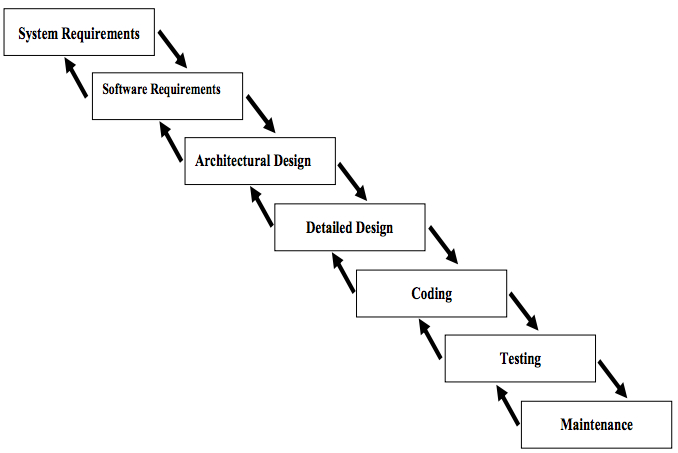
\includegraphics[scale=0.7]{Picture/waterfall.jpg}
\caption{Waterfall model}
\label{fig:waterfall} % 
\end{figure}

\section {Scrum}
\label{sec:Scrum}
"Scrum is the best-known of the Agile frameworks. It is the source of much of the thinking behind the values and principles of the Agile Manifesto" \parencite{Scrum}.

The Scrum method relates to value as
\\ 
\begin{center} \textbf{Individuals and interactions}  \textit{over processes and tools} \\
\textbf{Working software} \textit{over comprehensive documentation} \\
\textbf{Customer collaboration} \textit{over contract negotiation} \\
\textbf{Responding to change} \textit{over following a plan} \\
\end{center}

%"Individuals and interactions over processes and tools", "Working software over comprehensive documentation", "Customer collaboration over contract negotiation" and "Responding to change over following a plan" from the Agile Manifesto\parencite{Scrum}. 

These principles are not so rigid as the principles of the Waterfall method. Some may say that Scrum is the opposite of the Waterfall method \parencite{cocco2011simulating}. 

Scrum have three main roles, the Product Owner, the Scrum Master and the members of the development team. The Product owner in collaboration with the Scrum Master decides which work to be prioritized in the backlog. The backlog represents the tasks to be done in order to complete the project. The Scrum Master acts like a team leader and helps the development team and the organization to take best advantages of Scrum. The development team works on tasks specific for the sprint there in \parencite{Scrum}.

Sprint is a time-boxed interval over a given time. The Scrum framework suggests duration of sprints to be from one to four weeks. Before each sprint, a sprint planning meeting is conducted with all the team members attending.  A Sprint planning meeting is held so the team can discuss tasks from the backlog and come to an agreement of which tasks to be put in the minimal backlog \parencite{Scrum}.

In each sprint a minimal backlog is created so the developer knows which tasks to work on in the current sprint. The Product Owner and the team members discuss and decide which tasks from the backlog to be added to the minimal backlog. After the minimal backlog is complete, the Product Owner and the team members discuss each task in order to get a better and shared understanding of what is required in order to complete the tasks \parencite{Scrum}. 

One of the main principles in Scrum is that it requires that a new feature is ready for release after each sprint. The feature should be a visible part of the product in order to get feedback from end-users. So all the tasks in the minimal backlog combined should be a visible part of the product.  \parencite{Scrum}.


\section {Lean}
\label{sec:Lean}
"Lean is all about getting the right things to the right place at the right time the first time while minimizing waste and being open to change" \parencite{741480}

The Lean approach was introduced around 1948 in manufacturing in Japan.  In 1975, Toyota was able to create almost 50 more production units per employee than in 1948 due to the Lean approach \parencite{manning}. Lean strives to maximize the value produced by an organization and delivered to costumer. This is done by finding and eliminate waste, controlling variability and maximizing the flow of delivered software all within the culture of continuous improvements \parencite{DavidAnderson}. In 2003 Mary and Tom Poppendieck first introduced Lean thinking to software development. Poppendieck published the book "Lean Software Development: An Agile Toolkit" \parencite{Lean:2003}. Poppendieck stated that an important tool to manage work flow is the concept of pull-systems, which means tasks are put in production only when a costumer asks for it \parencite{Lean:2009}.
The pull-system based method Kanban, has in the recent years been introduced more and more to software development, and is becoming one of the keys to Lean practice in software development \parencite{DavidAnderson}.  

There are eight fundamental principles in Lean. The eight principles are:
\begin{enumerate}
\centering
\item \textbf{Start Early:}  Don't wait for details. As soon as enough information is gathered start the development activity. Get everyone involved in figure out the details. Don't build any walls between people, make people collaborate and start a two-way communication as soon possible. This will start the learning cycle as well.

\item \textbf{Learn Constantly:} Start with a breadth-first approach, explore multiple options. The system is expected to change, so focus on creating simplicity code and robustness so the system is easy to change

\item \textbf{Delay Commitment:} 
In order to delay commitment, automated testing and refactoring are essential for keeping code changeable. 

\item \textbf{Deliver Fast:}
Deliver fast mark of excellent operational capability. The whole idea of \textbf{delaying commitment} is to make every decision as late as possible when one have the most knowledge.
\item \textbf{Eliminate Waste:}
The only thing worth doing is deliver value to the costumer, anything else is waste.  See waste and eliminate it is the first key of Lean.  Lean suggests using a value stream map for removing waste. A Value Stream Map (VSM) is a map over the whole company chain. VSM helps visualize where waste are located within the company.
\item \textbf{Empower the team:} When one are going to deliver fast, there is no room for central control. The work environment should be structured so work and workers are self-directing.

\item \textbf{Build Integrity In:} Lean software is build with integrity. That's why one of the principles in Lean suggests that test are integrated into software development just as any code, so it becomes a part of the delivered product. 

\item \textbf{Avoid Sub-optimization:} In software development it's normal to break down a complex problem into small parts of the problem in order to minimize the complexity.  If some of the parts are sub-optimized, bottleneck can occur. For example, if ten developers are hired to work on tasks, but only three testers are hired. The development process is sub-optimized since the developers will likely produce more than the tester can test and that will cause bottleneck.
\end{enumerate}
\parencite{poppendieck2003lean}

\section{Kanban}
\label{sec:Kan}
\iffalse
Shinkle defined novice and more experience kanban-users with a descriptive analogy \parencite{Shinkle}:
''Think about a typical person wanting to bake a cake. They go to the store, purchase a boxed cake mix, and follow the directions as described on the back of the box. They have little to no knowledge about how to alter the recipe nor do they have a desire to do so. Their goal is simply to bake a cake.''

''An advanced beginner understands how to apply some context to the instructions or rules on the back of the box. They can make minor adjustments for things like altitude, pan size, oven conditions, etc. They are still following the basic recipe, but can make minor adjustments likely based on previous experiences." According to Shinkle, principles like WIP limit will be adopted when the user has some experience with Kanban. 
\fi


''One can define Kanban software process as a WIP limited pull system visualized by the Kanban board''  \parencite{DavidAnderson}.

Toyota production system introduced Kanban as a scheduling system for Lean and just-in-time (JIT) production during late 1940's and in the early 1950's in order to catch up with the American car industry. The Kanban method combined with the Lean approach was a success for Toyota. The success was noticed by the software development industry among others \parencite{Conboy}, \parencite{ono1988toyota}. In the recent years, more software projects adapt to Kanban and Lean \parencite{DavidAnderson}, and this is one of the reasons why this thesis will focuses on Kanban and one of it's main principle WIP limit. 


One of the most important people in Kanban software development, David Anderson  also referred to as ''father of Kanban in the software development industry''  \parencite{InfoQ:2013:May:Online} and author of the book "Kanban: Successful Evolutionary Change for Your Technology Business" has stated ''If you think that there was Capability Maturity Model Integration, there was Rational Unified Process, there was Extreme Programming and there was Scrum, Kanban is the next thing in that succession.''   \parencite{InfoQ} 

In software development the Kanban method splits the major problem into many small pieces of problems. When the small pieces are defined by the team, the problems are put up on the Kanban board to visualize the problems, track what others are working on and see potential bottlenecks during development. Shinkle stated that when people start to understand Kanban, they easily discovered where the bottlenecks are \parencite{Shinkle}.

In short Kanban systems focus on:
\begin{itemize}
\item Continuous flow of work.
\item	No fixed iterations or sprints.
\item Work is delivered when it's done.
\item Teams only work on few tasks at the time specified by the WIP limit.
\item Make constant flow of released tasks.
\end{itemize}
\parencite{DavidAnderson}.


One of the main differences between Scrum and Kanban is sprint and estimation. Contrary to Scrum, Kanban do not use the principles of sprints or estimations. In Kanban the tasks do not need to be estimated or finished within a certain time. In the article "simulation of software maintenance process, with and without a work-in-process limit" \parencite{SMR:SMR1599} the authors found out that if they let the developers work with small tasks at time and not be interrupted, they will be more effective. They also found out that Scrum was too rigid for the development team because when the team had to estimate tasks they felt interrupted.  So the estimation and sprint meetings worked counterproductive. The authors made the developers change to Lean-Kanban.  The change implied the removal of sprints and estimation. After removing sprints and estimation the teams increased the ability to perform work, lower the lead time and meet the production dates \parencite{SMR:SMR1599}.

In the article "Quantifying the Effect of Using Kanban versus Scrum:" the company also felt that the Scrum approach was too rigid. The article also reported positive results when the team changed to Kanban.  The company almost halved its lead time, reduced the number of weighted bugs by 10 percent, and improved productivity \parencite{Dag}. Other article also states that Scrum is too rigid and that's Kanbans advantages over Scrum \parencite{beedle1999scrum} \parencite{brekkanintroducing} .  

\subsection {Kanban Board}
''The Kanban board makes it clear to all the team members the exact status of progress, blockages, bottlenecks and they also signal possible future issues to prepare for''\parencite{Joyce}.

The Kanban board is one of many tools in Kanban. It's used to control WIP, increase the information flow with visualization and spot bottlenecks \parencite{SMR:SMR1599}. A Kanban board is illustrated in figure \ref{kanban_board}. Each column in figure has \ref{kanban_board} an intuitive name in order to describe itself so the developers easily can track where each task is. 

Each column is named "Backlog", "In progress" and "Done".  Each column can have a WIP limit to specify how many works in progress there are allowed in the column \parencite{Joyce}. In figure \ref{kanban_board} the WIP limit is stated under the column name. The backlog column has a WIP limit of 4, In progress has 5 and Done doesn't need a WIP limit. 

The yellow stickers represent the tasks. Some follow the path to mark stickers with different colors representing the severities or by marking if its a feature or a bug. In "Kanban Implementation in a Telecom Product Maintenance" for example, the stickers has three different colors, green, yellow and red depending on how close to overdue the tasks are. If the sticker is red, the task is already overdue, if the tasks are soon-to-overdue its marked with yellow stickers \parencite{6068363}.
\begin{figure}[!htbp]
\centering
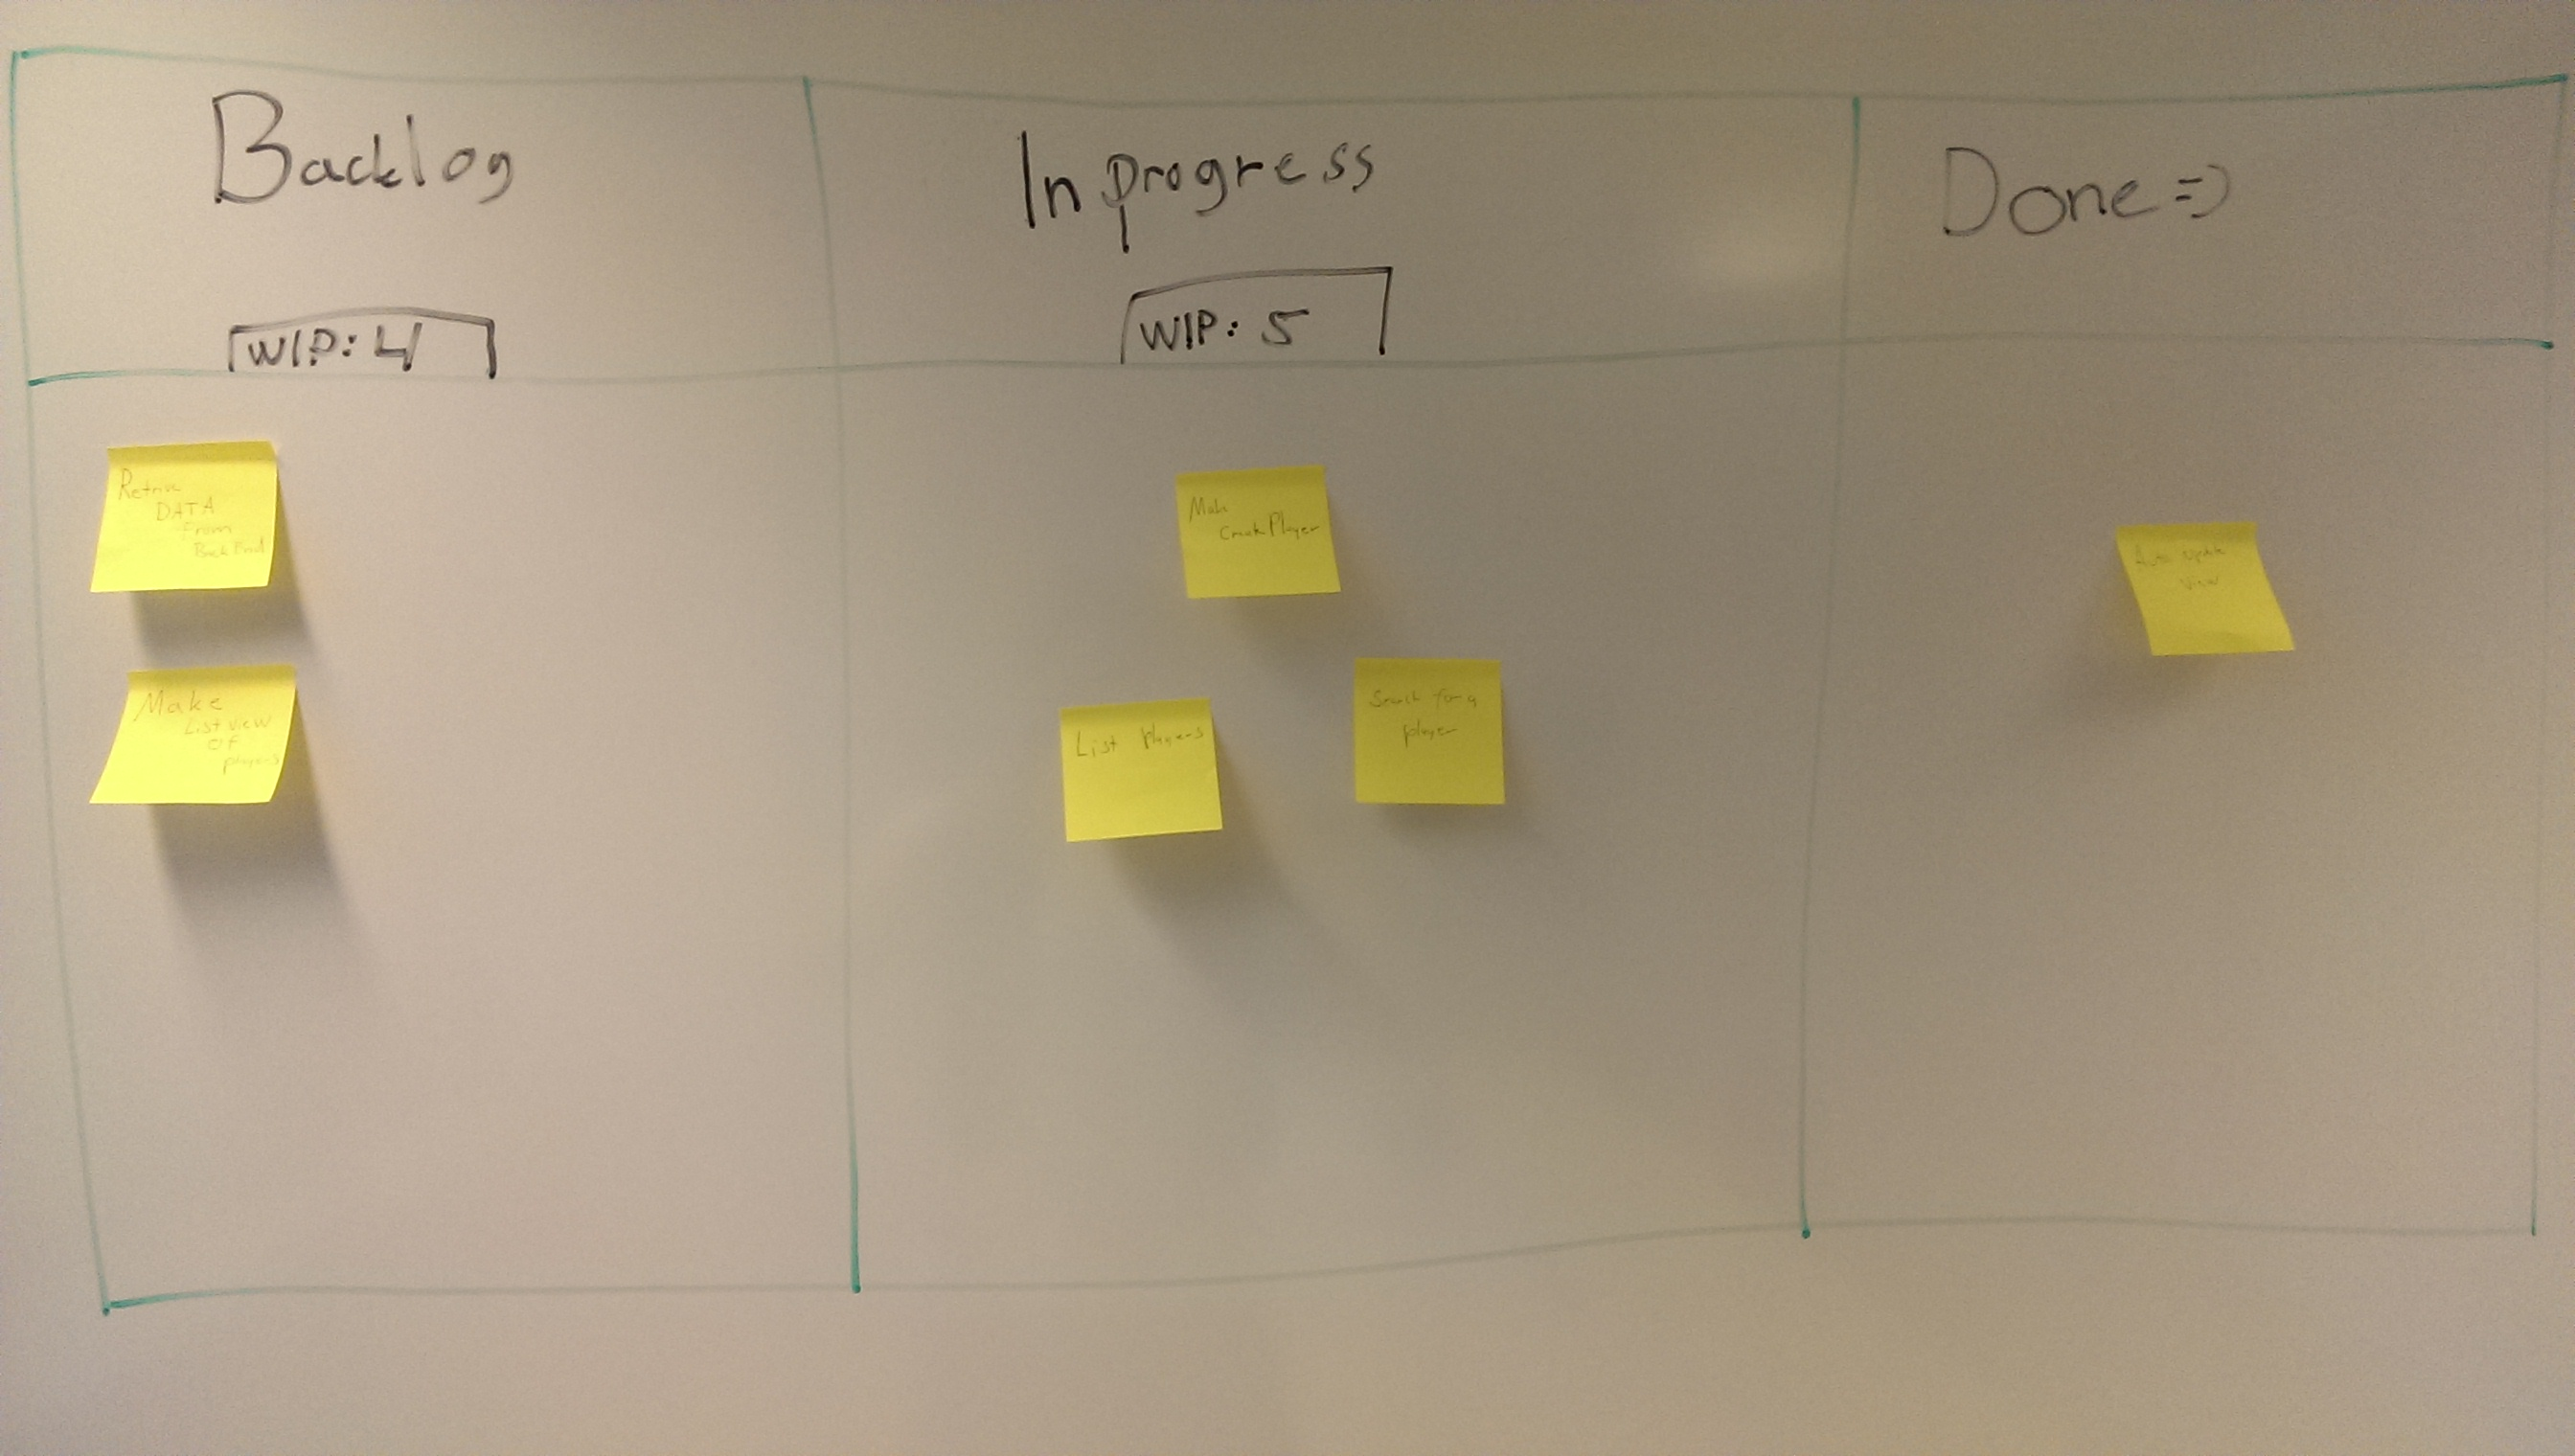
\includegraphics[width=90mm]{Picture/kanban_board.jpg}
\caption{Example of a Kanban board}
\label{kanban_board}
\end{figure}

\subsection{WIP limit}
\label{WIPsec}
''WIP limits seem to be the worst understood part of the Kanban system. When used properly, it exposes bottlenecks and reduces lead time for individual work items. Used improperly, it can starve developers for work or result in too many people working on the same work items.'' \parencite{Shinkle}

WIP limit is one of the core principles in Kanban \parencite{6068363}. WIP limit helps to reduce overhead by limit task-switching for each developer, visualize bottlenecks and make constant flow of tasks throughout the development \parencite{DavidAnderson}. One way to explain WIP and the impact of WIP limit is to use cars and roads as analogy. All roads have it maximum capacity of cars. When this limit is reached, traffic jam occurs and the throughput of cars decreases and lead time increases. The same can be said about software development teams. A software team has a maximum number of tasks they can perform, if the team is pushed over the maximum limit, the throughput of tasks decreases and lead time increases.

When first implementing Kanban, Shinkle explains that the users don't care about WIP or setting a WIP limit, but rather the visibility of Kanban through the Kanban board. When user get more experience with Kanban, they start to attempt the principles of WIP limit \parencite{Shinkle}. Srinivasan, Ebbing and Swearing said that setting the WIP limit is not easy. They suggest that the WIP limit is set, and then observe throughput, and adjust after that \parencite{Mandyam}. The Kanban method also says you should limit WIP, but what should the limit be? The Kanban method tells us to experiment \parencite{Kniberg}. The article "Lean Software Management" \parencite{Kniberg} and the "Impact of Kanban on Software Project Work" \parencite{Ikonen} both suggest that WIP should be minimized as well. The conclusion of present study is to keep the WIP limit low and experiment by slowly increase the WIP limit until the throughput decreased and lead time increased, then you know that the previous WIP limit was the perfect one.

The importance of limit WIP has been stated by various researches. A summary of benefits with WIP limit is shown in section \ref{sub:sub:benefits} .  The articles by Giulio Concas, Hongyu Zhang \parencite{SMR:SMR1599}  and David Anderson, Giulio Concas, Maria Ilaria Lunesu, and Michele Marchesi \parencite{DavidAnderson} researched the difference between limit WIP and unlimited WIP.  A summary of this two articles are shown in section \ref{sub:wip:vs:wip}

On how to determine WIP limit one research was found. If one implement Kanban with sprints or uses Scrum, \L ukasz proposes to use the effectiveness metric to help determine the WIP limit. The effectiveness metric should be applied after end sprint according to \L ukasz. After each sprint, one can apply the effectiveness metric and the result could be used as a guideline for WIP limit for the next sprint. The effectiveness metric takes the number of bugs found (ai) and the number of bugs found by external people (e.g. lawyers, accountants, coaches, consultants, translators, internal and external service providers etc.) (ei), and minus ai and ei, then divide the result by ai and multiply it by 100\%  as shown in \ref{WIPEQ} \parencite{Sienkiewicz}

\begin{equation} \label{WIPEQ}
Ei=\frac{(ai-ei)}{ai}*100\%
\end{equation}

\subsection {Limit WIP vs. Unlimited WIP}
\label{sub:wip:vs:wip}
In the article by Giulio Concas and Hongyu Zhang one of the result was showed that the average of closed tasks was 4145 when the WIP was limited and 3853 when the limit was not limited (about 7\% less). The paper concludes their finds; developers are more focused on fixing few issues, because the number of issues they can work on is limited. The developers are more likely to continue on the issue from the day before, rather than starting on another issue, this reduces overhead. When developers start on a new issue, they need to use time to familiarize themselves with the code and the issue. That could create unnecessary overhead if some developer already has done it, but that developer is now working on another issue. The study also showed that limit WIP can improve throughput and work efficiency \parencite{SMR:SMR1599}.

The case by David Anderson et al. \parencite{DavidAnderson} did a simulation of the impact of WIP limit vs. no WIP limit on developers with skills in different activities. The four skill activities from the article where:
\begin{enumerate}
\item Design
\item Development
\item Testing
\item Deployment
\end{enumerate}

The article did four different simulations. 
\begin{enumerate}
\item A simulation with WIP limits and seven developers with skill in two of the four activities. 
\item A simulation with no WIP limit and seven developers with skilled in two of the four activities. 
\item A simulation with WIP limits and seven developers with skill in all of the activities.
\item A simulation with no WIP limits and seven developers with skill in two of the four activities.
\end{enumerate}
The research paper concluded that the two latter is unlikely in the real world, since there is seldom a whole team with developers skilled in all activities.
 
When the developers had skill in two out of four activities the WIP limit simulation used 100 days, but the non WIP limit simulation used 120 days. The simulation with WIP limit shown an almost constant flow of features that where completed. While in the same simulation with no WIP limit, the flow of feature was much more irregular.  
\parencite{DavidAnderson}

\subsection{Benefits with setting WIP limit according to various articles}
\label{sub:sub:benefits}
\begin{enumerate}
\item Lowering the WIP limit will help people avoid task switching. When one is task switching it's hard to be able to fully concentrate. \parencite{Ikonen}.
\item There's stated when using short-cycle times and Kanban board to limit WIP, the software development team's learning is increased \parencite{Joyce}:
\item In the article "Lean Software Management: BBC Worldwide Case Study", the team started to determine WIP by their constraints and quickly find their bottlenecks; this gave the team more experience in dealing with WIP and increased productivity\parencite{Joyce}.
\item Limit WIP helps team to reduce overhead \parencite {CONWIP}.
\item Limit WIP decrease lead time \parencite {CONWIP}.
\item Limit WIP increase throughput \parencite {CONWIP}.
\item Limit WIP reduces flow times \parencite {CONWIP}.
\item Limit WIP reduces variation \parencite {CONWIP}.
\item Limit WIP improves quality \parencite {CONWIP}.
\end{enumerate}

Both the studies on WIP limit vs. No limit and the articles and research shows the importance of WIP limit. If  \L ukasz's effectiveness metric is disregard, there is no clear rule on how to determine WIP limit even though WIP is a crucial principle in order to take full advantages of Kanban.

\section {Lead time}
''Lead time is the total elapsed time from when a customer requests software to when the finished software is released to the customer'' \parencite{Joyce}.

Lead time is an essential ingredient when you look for the optimal WIP. Often in project, lead time is split into pieces, so every task has its own lead time. This gives the development teams the advantages to experiment with different WIPs in order to see the different lead times and then measure which WIP that suits this project the best. 

The citation by Middleton and Joyce above is close to definition of what lead time is. This definition could be useful for consultancy companies, but for in-house development company with few releases each year this definition is unsuitable. The article "Quantifying the effect of Using Kanban versus Scrum" \parencite{Dag} stated some reasons why this is unsuitable for in house development companies: 

"First, the amount of time a work item remains in the backlog queue before it's put on the board is a function of priority, not whether the company uses Scrum, Kanban, or other development methods. Furthermore, companies that develop and sell products to many customers might propose new features themselves and put them on the backlog before any customers request them. Second, given a policy of two or three releases a year, the result of a work item isn't delivered to the customer immediately after it's finished'' \parencite{Dag}.


\section{Just-In-Time}
"Just-In-Time is based on delivering only the necessary products, to the necessary time and the necessary quantity." \parencite{JIT}.

Just-In-Time (JIT) was introduced in the 1970s by Toyota in combination with Lean \parencite{javadian2013just}.  JIT has been developed to increase productivity through waste reduction and increasing the value added on the production processes. To explain, illustrate and visualize the JIT principle Mary and Tom Poppendieck uses the picture shown in figure \ref{JITE}  \parencite{JIT} \parencite{Lean:2006}.

\begin{figure}[ht!]
\centering
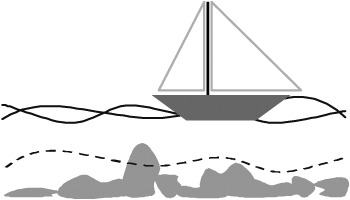
\includegraphics[width=90mm]{Picture/JIT.jpg}
\caption{JIT example}
\label{JITE} % JIT example
\end{figure}


In figure \ref{JITE} the stream reflects the inventory.  Under the stream, there are rocks located in different sizes. The rocks illustrates waste and problems that can occur.  If the stream level is lowered, the rocks are more visualized. At this point you have to clear out rocks in order to make the boat continue it's journey, or it will crash into the rocks. After the rocks are cleaned out, one can lower the stream level again and continue until it's just pebbles left. Then the boat can float without problems.

If one lower the stream (inventory), problems and waste will become visible (visualized by rocks). Lean want to lower inventory in order to make problems and waste occur, because when problems and waste occurs, you are able to fix the problems and remove the waste. Fixing the problem and removing the waste has several benefits such as, your process could be optimized and you are on step closer to have zero problems and zero waste.  \parencite{JIT} \parencite{Lean:2006}.

In Software development the JIT principle means that one should not deliver anything before it's demand. For example if a development team adds two new features to a product without consulting the stakeholders and work a day on these features. When stakeholders review the product they may say that they don't want the two features that, and that's waste. 

\section{Throughput}
''The output of a production process (machine, workstation, line plant) per unit time (e.g., parts per hour) is defined as the systems throughput or sometimes throughput rate'' \parencite{Adams}

The main concept of throughput is to measure how productive teams, people or companies are. Throughput is measured in number of finished delivered tasks or units per hour, day, week, month, quarter or year. This applies to both software development and manufacturing. The tasks in manufacturing are often different from the tasks in software development. In software development each task is more abstract than in manufacturing and in software development each tasks can have different solutions depending on how the team or developer approaches the task \parencite{Throughput}.

A key factor in successfully measuring throughput in software development is to specify a standard size for each task. If the standard is not specified a developer x can have throughput of one task per week, another developer y could have throughput of three tasks per week and they still have done the same amount of work, since the task of developer x is the same work amount as the three to developer y combined.  This will give wrong results if the throughput is measured \parencite{Throughput}. An example of throughput is listed in subsection \ref{sub:sub:throughput}. 

\subsection{Example of throughput measurement}
\label{sub:sub:throughput}
This is a simple example to illustrate throughput with different task sizes. Lets say Team x had a throughput of eighteen tasks after the first quarter, twenty after the second, fifteen after the third and twelve after the last quarter and they used Scrum the first two quarters and Kanban the last two as illustrated in table \ref{tt}. It will look like team x benefits most from Scrum. But if the task during the Kanban time was twice the size of Scrum, Kanban would suite team x the best. In order to get valid result from throughput measurements the size of tasks has to be agreed upon by the teams or company.
\begin{table}[ht]
\begin{center}
    \begin{tabular}{| l | l | l | l |}
    \hline
    Quarter & Throughput & Method\\ \hline
    1 & 18 & Scrum\\ \hline
    2 & 20 & Scrum \\ \hline
    3 & 15 & Kanban\\ \hline
    4 & 12 & Kanban\\ \hline
    \end{tabular}
\caption{Throughput}
\label{tt} %% throughput table
\end{center}
\end{table}

\section{Code churn}
\label{sec:Churn}
"Churn is defined as the sum of the number of lines added, deleted, and modified in the source code" \parencite{Dag}.

Churn is a measure that's not so quite known as lead time, throughput or WIP. Churn is a term that's used as surrogates for effort in software engineering. Many studies in software engineering use code churn or revisions as surrogate measure of effort \parencite{yamashita2012quantifying}. Emam stated that "analysts should be discouraged from using surrogate measures, such as code churn, unless there is evidence that they are indeed good surrogates \parencite{el2000methodology}."  The authors of "Quantifying the effect of code smells on maintenance effort" agree that one should cautious when using surrogates for effort. 



\section{Software Innovation}
\label{sec:SI}
Software Innovation(SI) is a Scandinavian software company. SI develops and delivers market-leading Enterprise Content Management applications that helps organizations improve and increase efficiency in document management, case handling and technical document control. SI builds products around Microsoft Sharepoint platform and tightly integrated into the Microsoft Office environment \parencite{Dag}. \parencite{SI}.

SI has approximately 300 employees in Oslo, Copenhagen and Stockholm and Bangalore \parencite{SI}. From 2001 to 2006, SI used Waterfall process. In 2007 SI changed to Scrum and in 2010 SI went from Scrum to Kanban \parencite{Dag}.



\chapter{Research Methods}
\label{chap:RM}
In this chapter the research methods will be introduced and the reason why the data from Software Innovation is used in this master thesis will be stated. The first section in this chapter, Section \ref{sec:CS} will give a brief introduction to the research method "Case Study".  Section \ref{sec:coc} is about the choice of case and complementary information about SI. 


\section{Case study}
\label{sec:CS}
To answer the research questions, a case study will be conducted.  A case study is used to explore causation in order to find underlying principles of a study \parencite{0078285763}\parencite{9781412960991}.  But which methods one can use in a case study or how the case study is conducted is ambiguous.  It might be that the case study is qualitative or quantitate.  Or that it utilizes a particular type of evidence (for example ethnographic, participant observation or field research). 

Jennifer Platt stated: "Much case study theorizing has been conceptually confused because too many different themes have been packed into the idea "case study" "\parencite{0521676568}.  

John Gerring stated: "A case study may be understood as the intensive study of a single case where the purpose of that study is - at least in part to shed light on a larger class of cases  \parencite{0521676568}.


%John also stated: "Case connotes a spatially delimited phenomenon (a unit) observed at a single point in time or over a period of time"\parencite{0521676568}. 

As one can see there is no clear rule what exactly a case study is. In this thesis the case study is used to explore WIP limit's effect in software development.  And the purpose is to shed light on WIP limit in software development and if it matter. In order to do so, the data set from SI with quantitative data will be interpreted.

\section{Choice of case}
\label{sec:coc}
The case study in this thesis is based on data set from an in house software company named Software Innovation. The data set contains information about each task SI has worked on in the last five years (2008-2013). The data set is represented in a excel document, a excerpt of some of the columns in the document is shown in table \ref{dataset}.
Skrive her at data fra 2010 og utover er tatt med, samme som i artikkelen til Dag, de har fjernet en del. 
\begin{table}[!ht]
\begin{center}
\begin{tabular}{|l|l|l|l|l|l|l|}
    \hline
    ID	& Type &  Created Date & From Day & Date To & Lead Time & Team \\ \hline
    3027 & Bug & 2008-10-07 &  2008-10-09 & 2008-10-16 & 20 & Team one\\ \hline
    3028 & Bug  & 2008-10-07 & 2008-10-07 & 2008-10-08 & 10 & Team six\\ \hline
    3029 & Feature & 2008-10-07 &  2008-12-30	 & 2008-12-30 & 105 & Team two\\ \hline
    3030 & Feature & 2008-10-07 & 2008-10-07	& 2008-10-07 & 1& Team three\\ \hline
    3035 & Bug & 2008-10-08 & 2008-11-20 & 2008-11-28 & 17 & Team five\\ \hline
    3037 & Feature & 2008-10-08 &  2008-10-19	 & 2008-10-19 & 7 & Team three\\ \hline
    3040 & Bug & 2008-10-10 &  2008-11-19 & 2008-11-19 & 48 & Team one\\ \hline
    \end{tabular}
\caption{Excerpt from the data set}
\label{dataset}
\end{center}
\end{table}
\newpage

In order to try answering the research questions stated in chapter \ref{chap:RQ}, the data from SI will be interpreted. The data set contains thirty columns with different data for each task, mostly of this columns are irrelevant for this study but the important columns is stated in table \ref{IC}.

The data from SI will be interpreted on team level.  SI has about 25 teams. From the data set there are six teams who have worked on the most tasks. The data from these six teams will be used. 
The data from SI will be analyzed using the program, which will compute the variables shown in table \ref{des} for each of the six team. This data will be further analyzed using SPSS. With SPSS the data produced by the program will be interpreted. The interpreted data will be presented in chapter \ref{ch:res}. 

The reason SI and the data set from SI is analyzed in this thesis is based on the article "Quantifying the Effect of Using Kanban versus Scrum" \parencite{Dag}. In the article the three authors investigated Kanban vs. Scrum in SI's case. Since Dag is the supervisor of this thesis and he had access to the data set, to use the set from SI is a choice of convenience. 

\begin{table}[!ht]
\begin{center}
    \begin{tabular}{| l | p{5cm} |}
    \hline
     Columns from data set & Description\\ \hline
     Created Date & When a task is put in backlog \\ \hline
     Date From & When a given task is pulled out from the backlog\\ \hline
     Date to & When a task is finished and ready for release. \\ \hline
    Lead Time & The amount of days elapsed from the date the task was created until the tasks has finished  \\ \hline
   Type & The type column is labeled as either bug or feature depending on the type of the task \\ \hline
   Lines added & Number of lines added to a feature or bug \\ \hline
   Lines modified & Number of lines modified when working on a feature or bug \\ \hline
   Lines deleted & Number of lines deleted from a bug or feature \\
    \hline
    Team &States the team who has been working on the task.\\ \hline
    \end{tabular}
\caption{Information about the columns from the SI dataset}
\label{IC} %% information columns
\end{center}
\end{table}

\newpage


\begin{table}[!ht]
\begin{center}
    \begin{tabular}{| l | p{5cm} |  p{5cm} |}
    \hline
    Variable &	Description	 & Columns from SI\\ \hline 
     WIP & \parbox[t]{5cm}{The number of items in progress on the given day} & Date From and Date To. \\ \hline
     Throughput	& Number of tasks finished on a given day & Date To \\ \hline
     Churn & Lines added, lines modified and lines deleted added together & Lines Added, Lines Modified, Lines Deleted and Date To \\ \hline
    Bugs & The number of tasks labeled as Bug and not feature & Type and Created Date \\ \hline
    Lead time & The time used on a task, measured in days & Lead time and Date To \\ \hline
  \end{tabular}
\caption{Relationship between variable and columns from SI}
\label{des} %% desription
\end{center}
\end{table}

\subsection{Software Innovation's development process}
From 2001 to 2006 SI used the Waterfall process with a life cycle of:
\begin{enumerate}[noitemsep,topsep=0pt,parsep=0pt,partopsep=0pt]
\item Design
\item Implementation 
\item Testing
\item Deployment for each new release
\end{enumerate} 
\parencite{Dag}. 

In 2007 SI examined their development process, which resulted in decision to change to Scrum. Scrum was implemented with the standard elements of Scrum:
\begin{itemize}[noitemsep,topsep=0pt,parsep=0pt,partopsep=0pt]
\item Cross functional teams
\item Sprint planning meetings 
\item Estimation of work items using planning poker
\item Daily standup meetings
\item Sprints
\end{itemize}
\parencite{Dag}. 

SI implemented three weeks sprint, after each sprint a fully tested shippable code was ready. In 2010, SI went from Scrum to Kanban. SI felt that Scrum was too rigid and didn't fit their purpose, they also feared that inaccurate estimation and time boxing gave them longer lead time. SI also saw Scrum planning meetings as waste which reduced productivity and quality \parencite{Dag}. 

SI decided to implemented Kanban in the following manner. When a work item is pulled from the backlog, SI tries to make the item flow through all the stages until it's ready for release. This procedure happens as quick as possible. In order for an item to be ready for release it has to be at a satisfactory quality level, which is defined by SI. SI also implemented WIP limits. If the WIP limit is reached, no new tasks are started until another task is finished which is based on the principle of just-in-time. \parencite{Dag}.



\chapter{Data collected and calculations}
\label{ch:DCC}
This chapter will introduce complementary information about the data set and the program. The first section, Section \ref{WPD} will introduce the algorithm of how the program measure WIP for each day. The subsection \ref{sec:Example} will provide a comprehensive example of how the program measure WIP per day. The consecutively sections reveals the algorithm of how the program measure bugs (Section \ref{sec:bug}) throughput (Section \ref{sec:TP}),  churn (Section \ref{sec:churn}) and lead time (Section \ref{sec:LT}). In the last section the statistical analyze program SPSS is introduced (Section \ref{sec:SPSS})

Keep in mind that each of these sections is not executed at the same time. Each of the sections represent one process in the program, and each of these processes have their own instance of the data set.


For this thesis a program was made in order to measure the variable shown in table \ref{des}. The explanation of how the program works will be split into sections so it will be easier to get a understanding of how the program operates. The explanation of how the program works will first contain a detailed description in words, then a description using Pseudocode \parencite{jd} will be provided. The Pseudocode for each section is simplified with only the key elements of the program code. 

The table \ref{tab:measurementDone} shows how quarters, dates and days are represented in this thesis. 

\begin{table}[!ht]
\centering
\begin{itemize}
\item The Date standard is specified as YYYY-MM-DD.
\item All seven days in the week are taken into account when measuring included Saturdays and Sundays
\item Quarter of a year is defined as: 
\begin{itemize}
\item January, February and March (Q1)
\item April, May and June (Q2)
\item July, August and September.(Q3)
\item October. November and December (Q4)
\end{itemize}
\parencite{Quarter}
\caption{The standard of the data set}
\label{tab:measurementDone}
\end{itemize}
\end{table}






%%legge inn en section her go ha de andre under her som subsection?
\section {WIP per day}
\label{WPD}

%% Table \ref {dataset} show an excerpt from the SI dataset.  The date 2008-10-09 is not in the set so the the program has to create 2008-10-09 and add it to the set in order to calculate WIP, throughput, bugs and lead time per day.  Skrive her at program lager hver dato for set self

\subsection{Step 1: Gather all unique dates into a Arraylist}
\label{sub:stepOne}
First step of WIP measurement is to create a WIP object with the attributes in table \ref{tab:object}.  The values that are assigned to the attributes are gathered from the data set file.  The program creates a WIP object and assigned values to it a shown in listing \ref{lst:Arraylist} . After the values are assigned the program puts it into the right Arraylist\footnote{Arraylist is a resizable array implementation of a list. The Arraylist class provides function for manipulate the size of the array, check the size of the list and convert the list to an array  \parencite{Arraylist}} based on the team variable as shown in listing \ref{lst:addWIP}

\begin{table}[!ht]
\begin{center}
\begin{tabular}{| l | l |}
\hline
Type & Variable name \\ \hline
Date & start \\ \hline
Date & end\\ \hline
String & team\\ \hline
String & processType\\ \hline
int  & WIP\\ \hline
\end{tabular}
\caption{Variables of the WIP objects}
\label{tab:object}
\end{center}
\end{table}


\begin{minipage}{\textwidth} 
 \begin{lstlisting}[caption={Gather all unique dates into Arraylist},label={lst:Arraylist}]
While inputFile != EOF // EOF = End Of file
		WIP = New WIP()
		WIP.start = inputFile.start
		WIP.end = inputFile.end
		WIP.team = inputFile.team
		WIP.processType = inputFile.processType
		WIP.WIP = 1
		FindTeam(WIP)
 \end{lstlisting}
 \end{minipage}
 
 \begin{minipage}{\textwidth} 
 \begin{lstlisting}[caption={Gather WIP object to the right data structure},label={lst:addWIP}]
void FindTeam (WIP w) 
		if w.team EQUALS "TeamOne"
			TeamOne.add(w)
		if w.team EQUALS "TeamTwo"
			TeamTwo.add(w)
		if w.team EQUALS "TeamThree"
			TeamThree.add(w)
		if w.team EQUALS "TeamFour"
			TeamFour.add(w)
		if w.team EQUALS "TeamFive"
			TeamFive.add(w)
		if w.team EQUALS "TeamSix"
			TeamSix.add(w)
 \end{lstlisting}
 \end{minipage}
 
\subsection{Step 2: Gather the remaining dates}
 \label{sub:stepTwo}
The data set from SI contains dates from 2008 to 2013, but there are some dates missing which table \ref{dataset} shows. For example the date 2008-10-09 is missing. In order to generate WIP for each day the program has to create the dates that's not in the set. 
  
In order to create the remaining dates, the program takes the first date and the last date from each of the teams's Arraylist created in previous section (\ref{sub:stepOne}) as shown in listing \ref{lst:remaining} in line one and two. Then the program checks if all the dates between the first date and the last date are in the team's Arraylist. Each of the Arraylists are sorted on date. If the dates are not in the Arraylist, the program will put the date into the Arraylist as show in method addToArraylist on line ten to thirteen.
In order to keep the pseudocode simple, the generateWIP method stated in line twelve was omit. The genereteWIP method creates a new WIP object and returns it. 

\begin{minipage}{\textwidth} 
\begin{lstlisting}[caption={Gather the remaining dates.},label={lst:remaining}]
WIP first = Arraylist.get(0)//points to the first WIP object in the Arraylist 
WIP last = Arraylist.get(Arraylist.size()-1)//points to the last WIP object in the Arraylist 
Next_date //points to the next date
Next_date = first.getDate() // Next_date assigned before iteration
while Next_date NOT EQUALS last.getDate()
	New_date = Next_Date + 1 //Compute the next date
	AddToArraylist(New_date, first.getTeam())
	Next_date = New_date

void addToArraylist(Date d, String team)
	if d NOT CONTAINS IN Arraylist
		WIP = generateWIP(d, team)
		Arraylist.add(WIP) 
 \end{lstlisting}
   \end{minipage}

\subsection{Step 3 Measure WIP}
The Arraylist from section \ref{sub:stepOne}  and \ref{sub:stepTwo} now contains a WIP object for each date from 2008 to 2013 for each team. In this step the program will loop through each of the Arraylists. During the iteration each WIP object is extracted from the Arraylist and the WIP is measured. The two methods stated in line ten and eighteen respectively gather the current WIP (method in line ten) and finds out how many finished tasks (method in line eighteen) and returns the result. The result is used in line five to compute the current WIP. 

\begin{minipage}{\textwidth} 
\begin{lstlisting}[caption={WIP measurement},label={lst:measure}]
lastWIP =  0
for WIP Object IN Arraylist	
	if(DateNotMeasured(WIP.getStartDate()) == true)
		WIP_for_this_date = get_current_WIP(WIP.getStartDate())  
		WIP_measured = WIP_for_this_date - Nr_of_finishedDates(WIP.getStartDate) + lastWIP
		WIP.setWIP(WIP_measured)
		lastWIP = WIP_measured 

int get_current_WIP(Date date)
	current_WIP = 0
	for WIP in  Arraylist
		if date EQUALS WIP.getStartDate()
			Nr_of_dates_to_decrement++
return current_WIP
			 	
int Nr_of_finished_dates(Date date)
	Nr_of_dates_to_decrement = 0
	for WIP in Arraylist
		if date AFTER WIP.getEndDate() DO
			if date not picked
				Nr_of_dates_to_decrement++
				dateIsPicked(WIP)				
return Nr_of_dates_to_decrement 
 \end{lstlisting}
  \end{minipage}

\subsection{Example}
\label{sec:Example}
This section will provide a comprehensive example of how the WIP algorithm works.  
Figure \ref{wip_timeline}  shows tasks id's in the y-axis and dates in the x-axis. The green line indicates the duration of the task. The figure helps  visualizes how many WIPs there are for a given date. For example on the date 2008-10-12, tasks 3, 5 and 6 are in progress, which means the WIP is 3 for 2008-10-12.  

In this example dates from table \ref{wt:2}  will be used to illustrate how the algorithm measure WIP.  The figure \ref{wip_timeline} visualize WIP for each date.
%skrive om tabellen
\begin{figure}[ht!]
\centering
\hspace*{-1in}
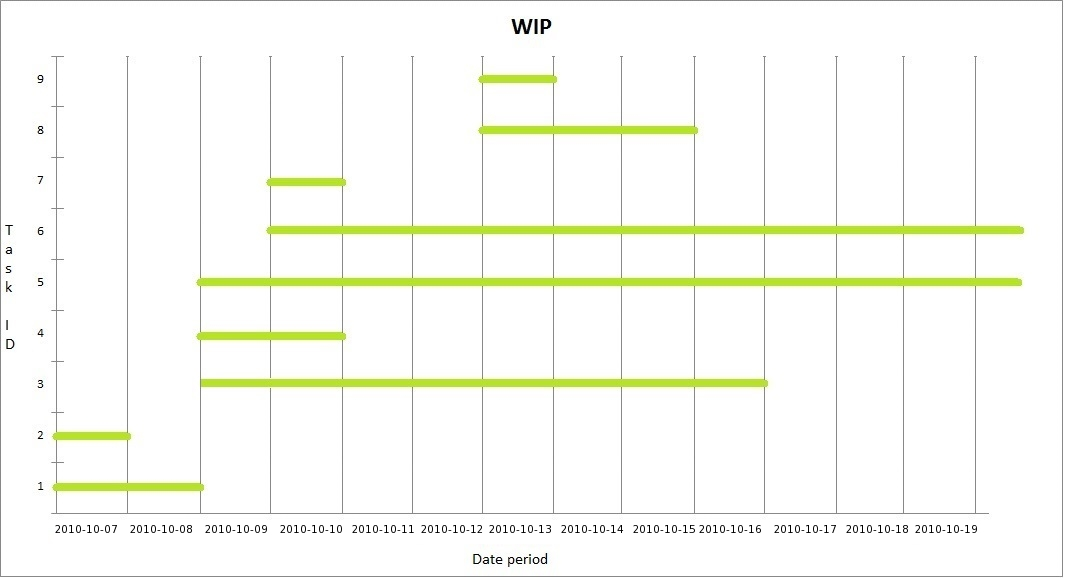
\includegraphics[width=21cm,trim=4 4 4 4,clip]{Picture/wip_example.jpg}
\caption{Illustrating the WIP timeline for example stated in section \ref{sec:Example}}
\label{wip_timeline}
\end{figure}

\newpage
\begin{table}[!ht]
\begin{center}
    \begin{tabular}{| l | l | p{2cm} | l | l |}
    \hline
   Task ID &   Date From  & Date To & Team & Process Type\\ \hline
     1 & 2008-10-07 & 2008-10-08 & Team One & Waterfall  \\ \hline
     2 & 2008-10-07 & 2008-10-07 & Team One & Waterfall   \\ \hline
     3 & 2008-10-09 & 2008-10-16 & Team One & Waterfall   \\ \hline
     4 & 2008-10-09 & 2008-10-10 & Team One & Waterfall   \\ \hline
     5 & 2008-10-09 & 2008-11-04 & Team One & Waterfall   \\ \hline
     6 & 2008-10-10 & 2008-11-05 & Team One & Waterfall  \\ \hline
     7 & 2008-10-10 & 2008-10-10 & Team One & Waterfall   \\ \hline
     8 & 2008-10-13 & 2008-10-15 & Team One & Waterfall  \\ \hline
     9 & 2008-10-13 & 2008-10-13  & Team One  & Waterfall   \\ \hline
    \end{tabular}
\caption{Showing Task ID, Date From and Date to}
\label{wt:2} %%  wip table 2
\end{center}
\end{table}

\subsubsection{Step 1}
The program will first read in the first line of table \ref{wt:2}.  The first line is the one labeled with task id one.  The program creates the WIP-object for line one and it will look like the listing \ref{lst:WIPOBJ}.  The program will follow the exact same procedure until all the dates are read in. 

\begin{minipage}{\textwidth} 
\begin{lstlisting}[caption={Creating WIP-object},label={lst:WIPOBJ}]
WIP = new WIP()
WIP.start = 2008-10-07
WIP.end = 2008-10-08
WIP.team = "Team One"
WIP.processType = "Waterfall"
WIP.WIP = 1
\end{lstlisting}
  \end{minipage}

 \subsubsection{Step 2}
\label{sub:sub:st}
Now that the whole set has been read in and saved. The next thing to do is to create the remaining dates. The Arraylist contains all the dates from table \ref{wt:2}.  The program will now extract the first and the last date from the Arraylist. Before this step, the objects in the Arraylist are sorted by date. The first date is 2008-10-07 and the last date is 2008-10-13.  The program will check if the date after 2008-10-07 contains in the set, which it don't. The program then generates a WIP object for the date 2008-10-08 and adds it to the Arraylist as shown in listing \ref{lst:WIPCREATE}. After the date is created, the program will see if the date 2008-10-09 exits and will do so for all dates until the date 2008-10-13.

\begin{minipage}{\textwidth} 
\begin{lstlisting}[caption={Creating WIP-object},label={lst:WIPCREATE}]
void createNewWIP(Date d, String team) 
	WIP.start = d
	WIP.end = d
	WIP.team = team
	WIP.processType = "Uknown"
	WIP.WIP = 0
\end{lstlisting}
  \end{minipage}


\subsubsection{Step 3}
The Arraylist now contains the dates from 2008-10-08 to 2008-10-13. The next and last step is to measure WIP for each date.  The program will now loop through the Arraylists. The first date is 2008-10-07.  The get\_current\_wip method from line nine in listing \ref{lst:measure} will be called with the date 2008-10-07 as parameter.  The method will return two, since both task one and two where started at 2008-10-07 as shown by figure \ref{wip_timeline}. The next thing to do is to find out how many tasks to decrement the current WIP with.  The method Nr\_of\_fininshed\_dates in line seventeen is called with the date 2008-10-07. As shown by the table \ref{wt:2} and figure \ref{wip_timeline} there was no task finished at the date 2008-10-07, so the method returns 0. The program then updates the WIP objects' counter to two and saves the WIP in the lastWIP object. The next date is 2008-10-08, who the program made in subsection \ref{sub:sub:st}. There is no task started at 2008-10-08, but task one is finished at the date. So the Nr\_of\_fininshed\_dates returns one and flag the current date at line twenty-three. The result of WIP\_measure in line five is 1 ($0-1+2=1$). WIP at date 2008-10-08 is one, as shown by figure \ref{wip_timeline}. The program will continue this procedure until all the dates are measured.  The reason why the date is flagged is to be sure that each day only evaluates ones. The if statement listed in listing \ref{lst:measure} at line twenty-one assurance that.

\iffalse
\subsubsection{First step}
\label{subsubsec:ft}
The program will first do a look-up on the date 2008-10-07 referred with task ID one and two in table \ref{wt:2} and measure the current WIP counter, which is two, because its two tasks in progress on this date. After this the program will put the date and the current WIP into a Arraylist. 
Now the algorithm will see if any task was done in the last period, since task one and two is the two first tasks to be measured in this example, there's no task finished in the period and there's no current WIP from other tasks, so the current WIP at 2008-10-07 is two illustrated by figure \ref{wip_timeline}. 
\subsubsection{Second step}
The program will do a look-up on the date 2008-10-09 referred with task ID three, four and five in table \ref{wt:2}  and measure the current WIP for this date, which is three. Then, the program will put the date and the current WIP into a Arraylist.
Next, the program will see that two tasks were done in the period of 2008-10-07 to 2008-10-09. So the program will measure that three new tasks were started at 2008-10-09, two where finished and the WIP from last date measure where two, so the calculation of WIP at 2008-10-09 is 3-2+2, which gives a WIP of three on 2008-10-09 illustrated by figure \ref{wip_timeline}. 

\subsubsection{Third step}
The program will do a look-up on the date 2008-10-10 referred with task ID six and seven in table \ref{wt:2}  and measure the current WIP for this date, which is two. Next the program will put the date and the current WIP into a Arraylist.
Last the program will see that no task where done in the period 2008-10-09 to 2008-10-10 and the currently WIP is three, so this gives a new WIP of 5 illustrated by figure \ref{wip_timeline}. 

\subsubsection{Fourth step}
The program will do a look-up on the date 2008-10-13 referred with task ID eight and nine in table \ref{wt:2}  and measure the current WIP for this date, which is two. Then the program will put the date and the current WIP into a Arraylist. 
Next the program will look at the period between 2008-10-10 and 2008-10-13, and see that task four and seven was done in this period. The WIP at 2008-10-13 will be $2-2+5 = 5$ as illustrated by figure \ref{wip_timeline}. 
As illustrated by the example, WIPs are not decrement until the finished date is passed, even though the task is done on the date, it's also worked on the same date, therefore the WIP is decrement after each date is passed.
\fi

\section {Bug}
\label{sec:bug}
Each task in the data set is label as either feature or bug as shown in figure \ref{bugsT}. When the program reads in the data file, each task label as bug are saved in a data structure. The code is shown in listing \ref{findBug}.

\begin{table}[ht]
\begin{center}
    \begin{tabular}{| l | l | p{5cm} |}
    \hline
    Task ID & Type \\ \hline
57970 &	Bug\\ \hline
57971&	Bug\\ \hline
57972&	Bug\\ \hline
57973&	Bug\\ \hline
57974&	Feature\\ \hline
57975&	Feature\\ \hline
57976&	Feature\\ \hline
57977&	Feature\\ \hline
57978&	Feature\\ \hline
    \end{tabular}
\caption{Example of how tasks are labeled}
\label{bugsT} %%  bugs table
\end{center}
\end{table}

\begin{minipage}{\textwidth}
\begin{lstlisting}[caption=Pseudocode example of how bugs are found, label=findBug]
void findBug()
	while inputFile != EOF //  EOF = End Of File
		newLine = readLine()
		if newLine.Type EQUALS 'Bug'
			B = New Bug()
			B.startDate = newLine.startDate
			B.process = newLine.process
			B.team = newLine.team 
			AddNewBug(B)
\end{lstlisting}
\end{minipage}
\subsection{Add Bug}
\label{addBugS}
When adding a new bug, each bug is gathered into a data structure based on team association, as the tests in lines 2, 7, 12 and 17 of the listing \ref{addBug} shows. After the right team is found the program tries to add the bug to the corresponding data structure as illustrated in lines 3, 8, 13 and 18. If the date of newly arrived bug already contains in the data structure, a counter representing the date is incremented and the new bug is discarded as shown the method dateExists in lines 26 to 32. 

Since the program knows which team the new bug belongs to (after the checks on line 3, 8, 13 and 18) a counter can represent number of bugs for each dates. In the analyze the only important is to know how many bugs there are on a given date and which team it belongs to.  

\begin{minipage}{\textwidth}
\begin{lstlisting}[caption=Pseudocode example of how bugs are added, label=addBug]
void addBug(Bug b)
	if b.team EQUALS "TeamOne"
		if dateExists(b.date, TeamOne) EQUALS false
			// if date don't exists, then add the bug
			TeamOne.add(b)
			
	if b.team EQUALS "TeamTwo"
		if dateExists(b.date, TeamTwo) EQUALS false
			// if date don't exists, then add the bug
			TeamTwo.add(b)
			
	if b.team EQUALS "TeamThree"
		if dateExists(b.date, TeamThree) EQUALS false 
			// if date don't exists, then add the bug
			TeamThree.add(b)
			
	if b.team EQUALS "TeamFour"
		if dateExists(b.date, TeamFour) EQUALS false
			// if date don't exists, then add the bug
			TeamFour.add(b)
		
void dateExists(Date d, Arraylist list)
	for Bug b in list
		if b.date EQUALS d
			b.counter++
			return true
	
return false	
 \end{lstlisting}
 \end{minipage}

 
\section{Throughput}
 \label{sec:TP}
Finding throughput per day is quite similar to how bugs are found (described in section \ref{sec:bug}).  When reading in the data set a new throughput object is created for each line in the data set smilier to how the bugs was created.  Then all throughput objects are sorted based on team association as shown in listing \ref{addBug} . When all throughput objects are gathered, the program measure throughput. The throughput measurement is similar to the dateExists method (lines 26 to 32) in the listing \ref{addBug} stated in section \ref{addBugS}. 

The dateExists method starts of with a test, the same test is done for bugs. If the date of the throughput object is in the data structure, the corresponding counter is incremented.  If the date is not in the data structure, the new throughput object is added to the data structure. An excerpt of the code is listed in \ref{throughputCode} 
\begin{minipage}{\textwidth}
\begin{lstlisting}[caption=Pseudocode example of how throughput is measured, label=throughputCode]
void dateExists(Throughput tp d, Arraylist list)
	for Throughput t in list
		if t.date EQUALS tp.date
			t.counter++
			return
			
structure.add(tp);
\end{lstlisting}
 \end{minipage}


\section{Churn}
\label{sec:churn}
As stated in section \ref{sec:Churn} in order to take churn into account one need to know it's good surrogates. SI has gathered churn with help of Microsoft's Team Foundation Server (TFS). The TFS system automatically records data such as churn and lead time. Based on TFS one can know that churn for SI is a good surrogate.

To measure churn the data set from SI contains three columns ("Lines added, "Lines modified" and "Lines deleted") shown in table \ref{table:churn}. These three columns are automatically recorded by TFS.  To complete the churn measurements the three columns are multiplied.  For task id one, the churn is 2028 ($352+307+1369 = 2028$). Some tasks has zero churn, for example task with id six, these tasks don't need code in order to be finished such tasks needs technical support to be finished.

%skal jeg skrive pseucode code til denne? 

\begin{table}[!ht]
\begin{center}
    \begin{tabular}{| l | l | l | l |}
    \hline
    Task id & Lines added & Lines modified  & Lines deleted \\ \hline
1&352&307&1369\\ \hline
2&314 & 31 & 15 \\ \hline
3&314&31 & 15\\ \hline
4&62&327&153 \\ \hline
5&21&3&0 \\ \hline
6&0&0&0 \\ \hline
\end{tabular}
\caption{How churn is presented in the excel document}
\label{table:churn} %%  bugs table
\end{center}
\end{table}

\section{Lead time}
\label{sec:LT}
The program does not need to analyze  the lead time for each task. The lead time for each task is recorded by TFS. The lead time is representer in the data set as shown in table \ref{table:LT}. The program will gather all the tasks that are started on the same day and belongs to the same team and add up their lead time together as shown in code listing \ref{LTcode}.   
\begin{table}[!ht]
\begin{center}
\begin{tabular}{ | l | l | l | }
\hline
	ID & Type & Leadtime \\ \hline
	84096 &  Feature  & 1 \\ \hline
	84118 &  Bug  & 25 \\ \hline
	84096 &  Feature  & 7 \\ \hline
	84118 &  Bug  & 13 \\ \hline
\end{tabular}
\caption{How lead time is recorded in the excel document}
\label{table:LT} %%  bugs table
\end{center}
\end{table}

\begin{lstlisting}[caption=Pseudocode example of lead time is measured, label=LTcode]

addLeadTime(lead_time t, Arraylist list)
	for lead_time in list
		if lead_time.date EQUALS t.date
			lead_time.leadtime+= t.leadtime
			return
			
structure.add(t)
\end{lstlisting}

\section{Lead time and churn}
As in the article "Quantifying the Effect of Using Kanban versus Scrum" \parencite{Dag} to prevent outliers from having a large effect on the results, the top and lowest ten percent of lead time and churn are removed from the data set.

Churn is removed because a module or a feature, which consists of hundred or thousand lines of code could be removed without much work and in this thesis churn is used as surrogate effort to know the complexity of the task. Lead time is removed because some tasks could be given low priority due to lack of manpower in a given period or tasks could be labeled as not critical and the lead time of these tasks will effect the result.
 

\section{SPSS}
\label{sec:SPSS}
"IBM® SPSS® Statistics is a comprehensive system for analyzing data. SPSS Statistics can take data from almost any type of file and use them to generate tabulated reports, charts and plots of distributions and trends, descriptive statistics, and complex statistical analyses." \parencite{IBM}

After the program has finished the measurements of the data, SPSS will be used to analyze the derived data. SPSS will help to answer the research question stated in chapter \ref{chap:RQ} with help of two statistics method: Correlation and case summaries. 





\chapter{Results}                     %% ... or ??
\label{ch:res}
\section{Introduction}
In this chapter 



\section{Correlation - WIP}
The table \ref{corr:WIP} shows the correlation between the seven teams and the WIP. The seven variables (T1-T7) shown horizontal in the table represents the seven teams from SI. T1 stands for team one, T2 for team two and so on. 

Some of the ten variables shown vertically are shown in table \ref{des} and are explained in chapter \ref{ch:DCC} ?Throughput Feature? means that tasks labeled with type ?feature? are the only one who is counted. For ?Throughput Bug? only the tasks labeled with type ?bug? is counted. The same goes for ?Churn Bug? and ?Churn Feature?. 

The ?Bugs finished in the same quarter? variable represents how many tasks labeled as bug that are finished within the same quarter as it was recorded.  The ?Average days for bugs in backlog? variable is used to see how long tasks labeled with ?bug? are in the backlog before pulled out. These two variables are used to see the prioritizing of bugs within a quarter as well as indicator of the workload for the quarter.   


Team one and four have a positive correlation between WIP and the throughput variables.  These two teams also have a positive correlation between WIP and bugs. 
Team three and six has positive correlation between WIP and lead time. Team five has a positive correlation with only the throughput bug variable. Team seven has a positive correlation between bugs finished in the same quarter and WIP.



\begin{table}[!htbp]
 \centering
 \begin{tabular}{|l|r|r|r|r|r|r|}
\hline
 & T1 & T2 & T3 & T4 & T5 & T6 \\ \hline
Throughput &.747**& 0.19& .717**& .815**& 0.53& .594*\\ \hline
Throughput Feature &.735**& -0.24& .828**& .895**& 0.14& .609*\\ \hline
Throughput bug &.625*& 0.30& .662**& .544*& .547*& 0.11\\ \hline
Bugs &.728**& 0.17& 0.53& .738**& 0.51& 0.43\\ \hline
Bugs finished in the same quarter &0.35& 0.27& -0.03& .581*& 0.20& 0.16\\ \hline
The average days for bugs in backlog &-0.02& 0.39& 0.41& 0.51& -0.18& 0.05\\ \hline
Leadtime &-0.23& 0.04& -0.11& .694**& 0.09& -0.09\\ \hline
Churn &-0.18& -0.30& -.569*& .c& -0.25& -0.03\\ \hline
Churn feature &0.38& -0.48& -0.44& .c& -0.02& 0.01\\ \hline
Churn bug &0.05& 0.13& -.671**
& .c
& -0.24& .775**
\\ \hline
\end{tabular}
 \caption{Correlation - WIP}
\label{corr:WIP}
 \centerline {* Correlation is significant at the 0.05 level (2-tailed).}
\centerline{** Correlation is significant at the 0.01 level (2-tailed).}
\centerline{c. Cannot be computed because at least one of the variables is constant.}
\end{table}



\section{Correlation - Leadtime}
\begin{table}[!htbp]
 \centering
 \begin{tabular}{|l|l|l|l|l|l|l|}
\hline
 & T1 & T2 & T3 & T4 & T5 & T6 \\ \hline
WIP &-0.23& 0.04& -0.11& .694**& 0.09& -0.09\\ \hline
Throughput &-0.44& -0.22& -0.39& 0.49& -0.19& -.554*\\ \hline
Throughput Feature &-0.35& 0.30& -0.34& .636*& -0.33& -0.52\\ \hline
Throughput bug &-0.27& -0.32& -0.31& 0.34& -0.14& 0.09\\ \hline
Bugs &-0.23& -0.23& -0.24& 0.44& -0.25& -0.22\\ \hline
Bugs finished in the same quarter &0.38& -.550*& 0.02& 0.48& -0.47& -0.36\\ \hline
The average days for bugs in backlog &-0.27& 0.44& -0.15& 0.13& 0.07& 0.01\\ \hline
Churn &0.41& -0.45& -0.13& .c& 0.24& -0.08\\ \hline
Churn feature &0.27& 0.41& 0.15& .c& -0.22& -0.20\\ \hline
Churn bug &0.28& -.725**
& -0.12& .c
& 0.25& -.553*
\\ \hline
\end{tabular}
 \caption{Correlation - Leadtime}
 \label{corr:Leadtime}
 \centerline {* Correlation is significant at the 0.05 level (2-tailed).}
\centerline{** Correlation is significant at the 0.01 level (2-tailed).}
\centerline{c. Cannot be computed because at least one of the variables is constant.}
\end{table}

\section{Correlation - Bugs}
\begin{table}[!htbp]
 \centering
 \begin{tabular}{|l|r|r|r|r|r|r|}
\hline
 & T1 & T2 & T3 & T4 & T5 & T6 \\ \hline
WIP &.728**& 0.17& 0.53& .738**& 0.51& 0.43\\ \hline
Throughput &.687**& .810**& .880**& 0.51& .975**& 0.27\\ \hline
Throughput Feature &.681**& -0.17& .744**& .619*& .825**& 0.25\\ \hline
Throughput bug &.925**& .856**& .867**& .590*& .957**& .744**\\ \hline
Bugs finished in the same quarter &0.50& -0.18& 0.12& .869**& 0.17& .762**\\ \hline
The average days for bugs in backlog &0.52& 0.38& 0.43& .533*& 0.18& 0.24\\ \hline
Leadtime &-0.23& -0.23& -0.24& 0.44& -0.25& -0.22\\ \hline
Churn &0.23& -0.01& 0.00& .c& -0.17& -0.10\\ \hline
Churn feature &0.30& 0.07& -0.03& .c& 0.28& -0.04\\ \hline
Churn bug &0.37& 0.17& -0.08& .c
& -0.19& 0.43\\ \hline

\end{tabular}
 \caption{Correlation - Bugs}
 \label{corr:bug}
 \centerline {* Correlation is significant at the 0.05 level (2-tailed).}
\centerline{** Correlation is significant at the 0.01 level (2-tailed).}
\centerline{c. Cannot be computed because at least one of the variables is constant.}
\end{table}


\section {Correlation - Throughput}
\begin{table}[!htbp]
 \centering
 \begin{tabular}{|l|r|r|r|r|r|r|}
\hline
 & T1 & T2 & T3 & T4 & T5 & T6 \\ \hline
WIP &.747**& 0.19& .717**& .815**& 0.53& .594*\\ \hline
Throughput Feature &.971**& -0.17& .846**& .947**& .775**& .991**\\ \hline
Throughput bug &.662**& .962**& .984**& .537*& .989**& -0.19\\ \hline
Bugs &.687**& .810**& .880**& 0.51& .975**& 0.27\\ \hline
Bugs finished in the same quarter &0.16& 0.12& 0.23& 0.39& 0.12& 0.12\\ \hline
The average days for bugs in backlog &0.16& 0.12& 0.45& 0.37& 0.14& -0.17\\ \hline
Leadtime &-0.44& -0.22& -0.39& 0.49& -0.19& -.554*\\ \hline
Churn &-0.27& -0.23& -0.26& .c& -0.20& -0.27\\ \hline
Churn feature &0.11& -0.18& -0.25& .c& 0.22& -0.23\\ \hline
Churn bug &-0.11& 0.06& -0.32& .c
& -0.21& .592*
\\ \hline

\end{tabular}
 \caption{Correlation - Throughput}
 \label{corr:TP}
 \centerline {* Correlation is significant at the 0.05 level (2-tailed).}
\centerline{** Correlation is significant at the 0.01 level (2-tailed).}
\centerline{c. Cannot be computed because at least one of the variables is constant.}
\end{table}

\section{Team 1 - Descriptive Statistics}
\begin{table}[!htbp]
  \begin{adjustwidth}{-2.5cm}{}
\subfigure[Descriptive Statistic -WIP]{
 \label{DS:WIP:1}
 \scalebox{0.85}{
  \begin{tabular}{ | l | r | r | r | r | r | r | }
 \hline
 Quarter &	N &	Mean &	Median & Std.Dev & Max	& Min\\ \hline
2010-3  & 117.0 & 0.8 & 0 & 1.5 & 5.0 & 0\\ \hline
2010-4 & 184.0 & 0.3 & 0 & 0.6 & 3.0 & 0\\ \hline
2011-1 & 180.0 & 1.7 & 0 & 5.1 & 30.0 & 0\\ \hline
2011-2 & 182.0 & 6.6 & 1.0 & 12.2 & 51.0 & 0\\ \hline
2011-3 & 184.0 & 0.9 & 0.5 & 1.0 & 3.0 & 0\\ \hline
2011-4 & 184.0 & 7.1 & 0.5 & 17.5 & 97.0 & 0\\ \hline
2012-1 & 182.0 & 11.1 & 2.0 & 15.1 & 67.0 & 0\\ \hline
2012-2 & 182.0 & 15.2 & 4.5 & 25.5 & 107.0 & 0\\ \hline
2012-3 & 184.0 & 18.0 & 9.0 & 20.4 & 65.0 & 0\\ \hline
2012-4 & 184.0 & 17.3 & 12.5 & 21.1 & 99.0 & 0\\ \hline
2013-1 & 180.0 & 16.4 & 12.5 & 19.1 & 85.0 & 0\\ \hline
2013-2 & 182.0 & 33.5 & 1.5 & 45.9 & 178.0 & 0\\ \hline
2013-3 & 184.0 & 3.7 & 0.5 & 7.2 & 31.0 & 0\\ \hline
2013-4 & 166.0 & 2.3 & 0 & 6.0 & 35.0 & 0\\ \hline
\end{tabular}
}
}
\subfigure[Descriptive Statistic -Throughput]{
 \label{DS:Throughput:1}
 \scalebox{0.85}{
 \begin{tabular}{ | l | r | r | r | r | r | r | }
 \hline
 Quarter &	N &	Mean &	Median & Std.Dev & Max	& Min \\ \hline
2010-3  & 3.0 & 3.0 & 1.0 & 3.5 & 7.0 & 1.0\\ \hline
2010-4 & 3.0 & 1.0 & 1.0 & 0 & 1.0 & 1.0\\ \hline
2011-1 & 7.0 & 10.4 & 11.0 & 8.1 & 25.0 & 1.0\\ \hline
2011-2 & 32.0 & 9.4 & 10.0 & 6.7 & 26.0 & 1.0\\ \hline
2011-3 & 2.0 & 1.0 & 1.0 & 0 & 1.0 & 1.0\\ \hline
2011-4 & 25.0 & 14.9 & 10.0 & 14.6 & 49.0 & 1.0\\ \hline
2012-1 & 49.0 & 8.6 & 5.0 & 8.1 & 33.0 & 1.0\\ \hline
2012-2 & 45.0 & 11.2 & 3.0 & 16.0 & 56.0 & 1.0\\ \hline
2012-3 & 34.0 & 5.5 & 3.0 & 6.3 & 23.0 & 1.0\\ \hline
2012-4 & 17.0 & 14.2 & 14.0 & 13.7 & 44.0 & 1.0\\ \hline
2013-1 & 13.0 & 19.5 & 17.0 & 17.0 & 58.0 & 1.0\\ \hline
2013-2 & 26.0 & 21.6 & 18.0 & 16.9 & 60.0 & 1.0\\ \hline
2013-3 & 17.0 & 9.0 & 7.0 & 7.7 & 27.0 & 1.0\\ \hline
2013-4 & 17.0 & 6.3 & 3.0 & 7.5 & 24.0 & 1.0\\ \hline
\end{tabular}
}
}
\end{adjustwidth}
\caption[Optional caption for list of figures]{Caption of Descriptive Statistic for WIP and Throughput  \subref{DS:WIP:1}, \subref{DS:Throughput:1}}
\label{DS:1:1}
\end{table}



%%%%%%%%%%%%%
% Leadtime and bugs
\begin{table}[!htbp]
  \begin{adjustwidth}{-2.5cm}{}
\subfigure[Descriptive Statistic - Leadtime]{
 \label{DS:LT:1}
 \scalebox{0.85}{
  \begin{tabular}{ | l | r | r | r | r | r | r | }
 \hline
 Quarter &	N &	Mean &	Median & Std.Dev & Max	& Min \\ \hline
2010-3  & 1.0 & 13.0 & 13.0 & . & 13.0 & 13.0\\ \hline
2010-4 & 2.0 & 8.5 & 8.5 & 9.2 & 15.0 & 2.0\\ \hline
2011-2 & 94.0 & 3.9 & 3.0 & 3.2 & 14.0 & 1.0\\ \hline
2011-3 & 1.0 & 5.0 & 5.0 & . & 5.0 & 5.0\\ \hline
2011-4 & 161.0 & 2.7 & 2.0 & 2.7 & 15.0 & 1.0\\ \hline
2012-1 & 231.0 & 3.6 & 3.0 & 3.1 & 15.0 & 1.0\\ \hline
2012-2 & 283.0 & 3.1 & 3.0 & 2.2 & 13.0 & 1.0\\ \hline
2012-3 & 96.0 & 3.3 & 1.0 & 4.0 & 15.0 & 1.0\\ \hline
2012-4 & 136.0 & 3.5 & 2.0 & 2.7 & 13.0 & 1.0\\ \hline
2013-1 & 115.0 & 3.1 & 3.0 & 2.0 & 10.0 & 1.0\\ \hline
2013-2 & 253.0 & 5.3 & 4.0 & 4.4 & 15.0 & 1.0\\ \hline
2013-3 & 85.0 & 4.6 & 4.0 & 3.0 & 13.0 & 1.0\\ \hline
2013-4 & 63.0 & 3.7 & 3.0 & 2.6 & 10.0 & 1.0\\ \hline
\end{tabular}
}
}
\subfigure[Descriptive Statistic - Churn]{
 \label{DS:Churn:1}
 \scalebox{0.85}{
 \begin{tabular}{ | l | r | r | r | r | r | r | }
 \hline
 Quarter &	N &	Mean &	Median & Std.Dev & Max	& Min \\ \hline
2010-3  & 1.0 & 13.0 & 13.0 & . & 13.0 & 13.0\\ \hline
2010-4 & 2.0 & 30.0 & 30.0 & 41.0 & 59.0 & 1.0\\ \hline
2011-2 & 94.0 & 21.5 & 10.0 & 22.9 & 83.0 & 1.0\\ \hline
2011-3 & 1.0 & 2.0 & 2.0 & . & 2.0 & 2.0\\ \hline
2011-4 & 161.0 & 17.5 & 8.0 & 23.1 & 94.0 & 0\\ \hline
2012-1 & 231.0 & 12.9 & 1.0 & 22.0 & 93.0 & 0\\ \hline
2012-2 & 283.0 & 12.9 & 1.0 & 22.2 & 92.0 & 0\\ \hline
2012-3 & 96.0 & 7.2 & 0 & 18.0 & 75.0 & 0\\ \hline
2012-4 & 136.0 & 4.1 & 0 & 12.2 & 67.0 & 0\\ \hline
2013-1 & 115.0 & 2.1 & 0 & 6.2 & 32.0 & 0\\ \hline
2013-2 & 253.0 & 7.6 & 0 & 15.7 & 92.0 & 0\\ \hline
2013-3 & 85.0 & 2.5 & 0 & 9.1 & 54.0 & 0\\ \hline
2013-4 & 63.0 & 4.3 & 0 & 16.2 & 90.0 & 0\\ \hline
\end{tabular}
}
}
\end{adjustwidth}
\caption[Optional caption for list of figures]{Caption of Descriptive Statistic for Leadtime and Churn  \subref{DS:LT:1}, \subref{DS:Churn:1}}
\label{DS:1:2} % 
\end{table}


  \begin{table}[!htbp]
 \centering
 \begin{tabular}{ | l | r | r | r | r | r | r | }
 \hline
 Quarter &	N &	Mean &	Median & Std.Dev & Max	& Min \\ \hline
2010-3  & 1.0 & 1.0 & 1.0 & . & 1.0 & 1.0\\ \hline
2010-4 & 4.0 & 1.0 & 1.0 & 0 & 1.0 & 1.0\\ \hline
2011-2 & 32.0 & 4.2 & 3.5 & 3.6 & 14.0 & 1.0\\ \hline
2011-3 & 5.0 & 1.0 & 1.0 & 0 & 1.0 & 1.0\\ \hline
2011-4 & 36.0 & 4.9 & 2.5 & 5.4 & 22.0 & 1.0\\ \hline
2012-1 & 43.0 & 3.5 & 3.0 & 2.3 & 10.0 & 1.0\\ \hline
2012-2 & 33.0 & 5.4 & 3.0 & 5.5 & 21.0 & 1.0\\ \hline
2012-3 & 16.0 & 2.4 & 1.5 & 1.8 & 6.0 & 1.0\\ \hline
2012-4 & 13.0 & 2.8 & 2.0 & 1.8 & 6.0 & 1.0\\ \hline
2013-1 & 8.0 & 3.5 & 3.0 & 2.5 & 7.0 & 1.0\\ \hline
2013-2 & 27.0 & 5.8 & 4.0 & 4.8 & 17.0 & 1.0\\ \hline
2013-3 & 11.0 & 1.3 & 1.0 & 0.5 & 2.0 & 1.0\\ \hline
2013-4 & 10.0 & 1.7 & 1.0 & 1.9 & 7.0 & 1.0\\ \hline
\end{tabular}
 \caption{Descriptive Statistic - Bugs}
 \label{DS:Bugs:1}
 \end{table}
 
 
 
\section{Team 2 - Descriptive Statistics}
\begin{table}[!htbp]
  \begin{adjustwidth}{-1.5cm}{}
\subfigure[Descriptive Statistic -WIP]{
 \label{DS:WIP:2}
 \scalebox{0.85}{
  \begin{tabular}{ | l | r | r | r | r | r | r | }
 \hline
Quarter &	N &	Mean &	Median & Std.Dev & Max	& Min \\ \hline
2010-3  & 117.0 & 3.1 & 0 & 6.6 & 23.0 & 0\\ \hline
2010-4 & 184.0 & 10.7 & 4.5 & 11.9 & 41.0 & 0\\ \hline
2011-1 & 180.0 & 13.6 & 8.5 & 14.1 & 38.0 & 0\\ \hline
2011-2 & 181.0 & 14.9 & 12.0 & 18.1 & 62.0 & 0\\ \hline
2011-3 & 184.0 & 16.3 & 9.0 & 17.6 & 56.0 & 0\\ \hline
2011-4 & 184.0 & 15.0 & 6.5 & 16.7 & 46.0 & 0\\ \hline
2012-1 & 182.0 & 10.0 & 4.0 & 10.6 & 31.0 & 0\\ \hline
2012-2 & 182.0 & 12.7 & 3.0 & 14.6 & 51.0 & 0\\ \hline
2012-3 & 184.0 & 12.1 & 5.5 & 13.4 & 45.0 & 0\\ \hline
2012-4 & 184.0 & 10.8 & 1.5 & 13.1 & 47.0 & 0\\ \hline
2013-1 & 180.0 & 9.9 & 4.0 & 10.7 & 35.0 & 0\\ \hline
2013-2 & 182.0 & 14.0 & 7.5 & 14.4 & 37.0 & 0\\ \hline
2013-3 & 184.0 & 9.4 & 4.5 & 9.9 & 28.0 & 0\\ \hline
2013-4 & 177.0 & 6.5 & 0 & 8.1 & 29.0 & 0\\ \hline
\end{tabular}
}
}
\subfigure[Descriptive Statistic -Throughput]{
 \label{DS:Throughput:2}
 \scalebox{0.85}{
 \begin{tabular}{ | l | r | r | r | r | r | r | }
 \hline
 Quarter &	N &	Mean &	Median & Std.Dev & Max	& Min \\ \hline
2010-3  & 16.0 & 4.2 & 3.0 & 4.0 & 16.0 & 1.0\\ \hline
2010-4 & 54.0 & 4.1 & 3.0 & 3.9 & 21.0 & 1.0\\ \hline
2011-1 & 57.0 & 4.6 & 4.0 & 3.6 & 17.0 & 1.0\\ \hline
2011-2 & 41.0 & 6.9 & 5.0 & 5.7 & 25.0 & 1.0\\ \hline
2011-3 & 52.0 & 3.8 & 2.0 & 3.6 & 15.0 & 1.0\\ \hline
2011-4 & 52.0 & 3.7 & 3.0 & 2.7 & 11.0 & 1.0\\ \hline
2012-1 & 55.0 & 4.3 & 3.0 & 3.4 & 12.0 & 1.0\\ \hline
2012-2 & 51.0 & 4.1 & 3.0 & 3.5 & 21.0 & 1.0\\ \hline
2012-3 & 57.0 & 5.8 & 5.0 & 4.3 & 18.0 & 1.0\\ \hline
2012-4 & 52.0 & 5.2 & 4.5 & 3.7 & 15.0 & 1.0\\ \hline
2013-1 & 51.0 & 4.6 & 3.0 & 3.6 & 16.0 & 1.0\\ \hline
2013-2 & 50.0 & 3.3 & 3.0 & 2.4 & 9.0 & 1.0\\ \hline
2013-3 & 55.0 & 3.9 & 4.0 & 2.9 & 16.0 & 1.0\\ \hline
2013-4 & 47.0 & 3.2 & 3.0 & 2.7 & 13.0 & 1.0\\ \hline
\end{tabular}
}
}
\end{adjustwidth}
\caption[Optional caption for list of figures]{Caption of Descriptive Statistic for WIP and Throughput  \subref{DS:WIP:2}, \subref{DS:Throughput:2}}
\label{DS:2:1} % 1 = team 2 = table nr 2
\end{table}

%%%%%%%%%%%%%
% Leadtime and bugs
\begin{table}[!htbp]
  \begin{adjustwidth}{-2.5cm}{}
\subfigure[Descriptive Statistic - Leadtime]{
 \label{DS:LT:2}
 \scalebox{0.85}{
  \begin{tabular}{ | l | r | r | r | r | r | r | }
 \hline
 Quarter &	N &	Mean &	Median & Std.Dev & Max	& Min \\ \hline
2010-3  & 33.0 & 8.6 & 5.0 & 8.1 & 24.0 & 1.0\\ \hline
2010-4 & 97.0 & 7.5 & 6.0 & 6.8 & 27.0 & 1.0\\ \hline
2011-1 & 133.0 & 7.2 & 7.0 & 5.3 & 27.0 & 1.0\\ \hline
2011-2 & 113.0 & 7.0 & 6.0 & 6.0 & 27.0 & 1.0\\ \hline
2011-3 & 98.0 & 8.8 & 6.0 & 6.8 & 27.0 & 1.0\\ \hline
2011-4 & 88.0 & 8.1 & 6.0 & 6.9 & 27.0 & 1.0\\ \hline
2012-1 & 128.0 & 5.6 & 4.0 & 5.0 & 27.0 & 1.0\\ \hline
2012-2 & 115.0 & 5.7 & 4.0 & 5.0 & 23.0 & 1.0\\ \hline
2012-3 & 212.0 & 6.0 & 5.0 & 4.7 & 22.0 & 1.0\\ \hline
2012-4 & 154.0 & 5.7 & 5.0 & 4.7 & 25.0 & 1.0\\ \hline
2013-1 & 136.0 & 6.5 & 5.0 & 5.5 & 24.0 & 1.0\\ \hline
2013-2 & 72.0 & 6.6 & 5.0 & 6.4 & 26.0 & 1.0\\ \hline
2013-3 & 100.0 & 6.7 & 5.0 & 6.0 & 27.0 & 1.0\\ \hline
2013-4 & 93.0 & 6.6 & 6.0 & 4.7 & 20.0 & 1.0\\ \hline
\end{tabular}
}
}
\subfigure[Descriptive Statistic - Churn]{
 \label{DS:Churn:2}
 \scalebox{0.85}{
 \begin{tabular}{ | l | r | r | r | r | r | r | }
 \hline
 Quarter &	N &	Mean &	Median & Std.Dev & Max	& Min \\ \hline
2010-3  & 33.0 & 56.7 & 10.0 & 97.9 & 352.0 & 1.0\\ \hline
2010-4 & 97.0 & 63.6 & 25.0 & 99.7 & 493.0 & 1.0\\ \hline
2011-1 & 133.0 & 41.6 & 18.0 & 66.2 & 407.0 & 1.0\\ \hline
2011-2 & 113.0 & 54.2 & 16.0 & 89.0 & 509.0 & 1.0\\ \hline
2011-3 & 98.0 & 53.6 & 25.0 & 78.2 & 379.0 & 1.0\\ \hline
2011-4 & 88.0 & 68.9 & 29.5 & 92.3 & 446.0 & 1.0\\ \hline
2012-1 & 128.0 & 68.8 & 23.0 & 96.0 & 521.0 & 0\\ \hline
2012-2 & 115.0 & 69.0 & 24.0 & 107.2 & 475.0 & 0\\ \hline
2012-3 & 212.0 & 63.3 & 24.0 & 92.0 & 442.0 & 0\\ \hline
2012-4 & 154.0 & 89.4 & 28.5 & 119.0 & 513.0 & 0\\ \hline
2013-1 & 136.0 & 54.0 & 12.0 & 92.5 & 467.0 & 0\\ \hline
2013-2 & 72.0 & 62.8 & 19.5 & 98.1 & 419.0 & 0\\ \hline
2013-3 & 100.0 & 88.2 & 33.5 & 120.5 & 514.0 & 0\\ \hline
2013-4 & 93.0 & 81.0 & 24.0 & 125.1 & 474.0 & 0\\ \hline
\end{tabular}
}
}
\end{adjustwidth}
\caption[Optional caption for list of figures]{Caption of Descriptive Statistic for Leadtime and Churn  \subref{DS:LT:2}, \subref{DS:Churn:2}}
\label{DS:2:2}
\end{table}

\begin{table}[!htbp]
 \centering
 \begin{tabular}{ | l | r | r | r | r | r | r | }
 \hline
 Quarter &	N &	Mean &	Median & Std.Dev & Max	& Min \\ \hline
2010-3  & 20.0 & 2.6 & 2.0 & 3.5 & 17.0 & 1.0\\ \hline
2010-4 & 40.0 & 2.5 & 2.0 & 1.7 & 9.0 & 1.0\\ \hline
2011-1 & 47.0 & 2.4 & 2.0 & 1.8 & 8.0 & 1.0\\ \hline
2011-2 & 40.0 & 3.8 & 3.0 & 2.5 & 13.0 & 1.0\\ \hline
2011-3 & 43.0 & 2.6 & 2.0 & 2.4 & 13.0 & 1.0\\ \hline
2011-4 & 47.0 & 2.5 & 2.0 & 1.6 & 8.0 & 1.0\\ \hline
2012-1 & 35.0 & 3.3 & 3.0 & 3.0 & 16.0 & 1.0\\ \hline
2012-2 & 34.0 & 2.3 & 2.0 & 1.5 & 7.0 & 1.0\\ \hline
2012-3 & 43.0 & 3.6 & 2.0 & 2.6 & 10.0 & 1.0\\ \hline
2012-4 & 33.0 & 3.9 & 3.0 & 3.1 & 14.0 & 1.0\\ \hline
2013-1 & 38.0 & 2.2 & 2.0 & 1.2 & 6.0 & 1.0\\ \hline
2013-2 & 32.0 & 1.9 & 1.5 & 1.2 & 5.0 & 1.0\\ \hline
2013-3 & 35.0 & 1.8 & 1.0 & 1.1 & 5.0 & 1.0\\ \hline
2013-4 & 37.0 & 1.9 & 1.0 & 1.3 & 7.0 & 1.0\\ \hline
\end{tabular}
 \caption{Descriptive Statistic - Bugs}
 \label{DS:Bugs:2}
 \end{table}

 \section{Team 3 - Descriptive Statistics}
 
 \begin{table}[!htbp]
  \begin{adjustwidth}{-1.5cm}{}
\subfigure[Descriptive Statistic -WIP]{
 \label{DS:WIP:3}
 \scalebox{0.85}{
  \begin{tabular}{ | l | r | r | r | r | r | r | }
 \hline
 Quarter &	N &	Mean &	Median & Std.Dev & Max	& Min \\ \hline
2010-3  & 116.0 & 1.9 & 0 & 4.8 & 23.0 & 0\\ \hline
2010-4 & 184.0 & 7.0 & 2.5 & 7.5 & 25.0 & 0\\ \hline
2011-1 & 180.0 & 7.7 & 3.5 & 8.2 & 23.0 & 0\\ \hline
2011-2 & 182.0 & 11.8 & 6.5 & 12.2 & 37.0 & 0\\ \hline
2011-3 & 184.0 & 10.4 & 4.5 & 11.2 & 34.0 & 0\\ \hline
2011-4 & 184.0 & 11.7 & 4.5 & 12.7 & 36.0 & 0\\ \hline
2012-1 & 182.0 & 12.5 & 6.5 & 13.3 & 42.0 & 0\\ \hline
2012-2 & 182.0 & 12.0 & 9.5 & 12.2 & 34.0 & 0\\ \hline
2012-3 & 184.0 & 14.0 & 10.5 & 14.5 & 38.0 & 0\\ \hline
2012-4 & 184.0 & 14.8 & 11.0 & 15.3 & 44.0 & 0\\ \hline
2013-1 & 180.0 & 8.1 & 4.5 & 8.9 & 27.0 & 0\\ \hline
2013-2 & 182.0 & 3.5 & 1.0 & 4.1 & 13.0 & 0\\ \hline
2013-3 & 184.0 & 3.5 & 1.5 & 3.8 & 14.0 & 0\\ \hline
2013-4 & 157.0 & 2.4 & 0 & 3.2 & 13.0 & 0\\ \hline
\end{tabular}
}
}
\subfigure[Descriptive Statistic -Throughput]{
 \label{DS:Throughput:3}
 \scalebox{0.85}{
 \begin{tabular}{ | l | r | r | r | r | r | r | }
 \hline
 Quarter &	N &	Mean &	Median & Std.Dev & Max	& Min \\ \hline
2010-3  & 16.0 & 3.3 & 3.0 & 2.9 & 12.0 & 1.0\\ \hline
2010-4 & 54.0 & 3.5 & 3.0 & 3.0 & 15.0 & 1.0\\ \hline
2011-1 & 42.0 & 2.2 & 2.0 & 1.4 & 7.0 & 1.0\\ \hline
2011-2 & 45.0 & 4.3 & 3.0 & 3.8 & 20.0 & 1.0\\ \hline
2011-3 & 51.0 & 4.0 & 3.0 & 3.4 & 15.0 & 1.0\\ \hline
2011-4 & 50.0 & 4.7 & 3.0 & 5.2 & 27.0 & 1.0\\ \hline
2012-1 & 46.0 & 6.5 & 5.0 & 5.7 & 20.0 & 1.0\\ \hline
2012-2 & 40.0 & 2.9 & 2.0 & 3.2 & 15.0 & 1.0\\ \hline
2012-3 & 36.0 & 3.4 & 2.5 & 3.1 & 13.0 & 1.0\\ \hline
2012-4 & 51.0 & 5.0 & 4.0 & 4.4 & 22.0 & 1.0\\ \hline
2013-1 & 42.0 & 3.2 & 2.0 & 2.9 & 10.0 & 1.0\\ \hline
2013-2 & 22.0 & 1.6 & 1.0 & 1.0 & 5.0 & 1.0\\ \hline
2013-3 & 29.0 & 2.0 & 1.0 & 2.0 & 11.0 & 1.0\\ \hline
2013-4 & 18.0 & 1.6 & 1.0 & 1.1 & 5.0 & 1.0\\ \hline
\end{tabular}
}
}
\end{adjustwidth}
\caption[Optional caption for list of figures]{Caption of Descriptive Statistic for WIP and Throughput  \subref{DS:WIP:3}, \subref{DS:Throughput:3}}
\label{DS:3:1}
\end{table}

 %%%%%%%%%%%%%
% Leadtime and bugs
\begin{table}[!htbp]
  \begin{adjustwidth}{-1.5cm}{}
\subfigure[Descriptive Statistic - Leadtime]{
 \label{DS:LT:3}
 \scalebox{0.85}{
  \begin{tabular}{ | l | r | r | r | r | r | r | }
 \hline
 Quarter &	N &	Mean &	Median & Std.Dev & Max	& Min \\ \hline
2010-3  & 31.0 & 7.2 & 7.0 & 4.1 & 16.0 & 1.0\\ \hline
2010-4 & 79.0 & 8.7 & 6.0 & 7.6 & 30.0 & 1.0\\ \hline
2011-1 & 32.0 & 7.4 & 4.5 & 5.7 & 18.0 & 1.0\\ \hline
2011-2 & 95.0 & 7.0 & 5.0 & 6.9 & 29.0 & 1.0\\ \hline
2011-3 & 90.0 & 7.7 & 5.0 & 7.0 & 30.0 & 1.0\\ \hline
2011-4 & 141.0 & 7.8 & 6.0 & 7.0 & 25.0 & 1.0\\ \hline
2012-1 & 171.0 & 7.8 & 6.0 & 6.7 & 30.0 & 1.0\\ \hline
2012-2 & 64.0 & 11.9 & 11.0 & 8.8 & 30.0 & 1.0\\ \hline
2012-3 & 71.0 & 9.6 & 8.0 & 7.5 & 27.0 & 1.0\\ \hline
2012-4 & 139.0 & 5.9 & 5.0 & 5.6 & 29.0 & 1.0\\ \hline
2013-1 & 75.0 & 7.1 & 5.0 & 7.7 & 29.0 & 1.0\\ \hline
2013-2 & 27.0 & 8.2 & 7.0 & 6.7 & 27.0 & 1.0\\ \hline
2013-3 & 32.0 & 6.9 & 4.0 & 7.9 & 29.0 & 1.0\\ \hline
2013-4 & 18.0 & 12.0 & 12.5 & 4.5 & 21.0 & 1.0\\ \hline
\end{tabular}
}
}
\subfigure[Descriptive Statistic - Churn]{
 \label{DS:Churn:3}
 \scalebox{0.85}{
 \begin{tabular}{ | l | r | r | r | r | r | r | }
 \hline
 Quarter &	N &	Mean &	Median & Std.Dev & Max	& Min \\ \hline
2010-3  & 31.0 & 145.0 & 118.0 & 143.8 & 383.0 & 1.0\\ \hline
2010-4 & 79.0 & 76.7 & 40.0 & 91.2 & 471.0 & 2.0\\ \hline
2011-1 & 32.0 & 81.6 & 62.0 & 74.0 & 320.0 & 2.0\\ \hline
2011-2 & 95.0 & 68.5 & 29.0 & 96.7 & 426.0 & 1.0\\ \hline
2011-3 & 90.0 & 72.7 & 22.5 & 102.5 & 476.0 & 0\\ \hline
2011-4 & 141.0 & 28.4 & 2.0 & 64.0 & 393.0 & 0\\ \hline
2012-1 & 171.0 & 44.5 & 2.0 & 82.7 & 475.0 & 0\\ \hline
2012-2 & 64.0 & 42.5 & 1.0 & 84.1 & 365.0 & 0\\ \hline
2012-3 & 71.0 & 53.9 & 13.0 & 85.3 & 406.0 & 0\\ \hline
2012-4 & 139.0 & 73.4 & 20.0 & 106.1 & 494.0 & 0\\ \hline
2013-1 & 75.0 & 45.4 & 10.0 & 68.8 & 291.0 & 0\\ \hline
2013-2 & 27.0 & 56.8 & 30.0 & 62.1 & 216.0 & 0\\ \hline
2013-3 & 32.0 & 66.1 & 34.5 & 87.2 & 403.0 & 0\\ \hline
2013-4 & 18.0 & 89.0 & 52.5 & 92.2 & 266.0 & 0\\ \hline
\end{tabular}
}
}
\end{adjustwidth}
\caption[Optional caption for list of figures]{Caption of Descriptive Statistic for Leadtime and Churn  \subref{DS:LT:3}, \subref{DS:Churn:3}}
\label{DS:3:2}
\end{table}


\begin{table}[!htbp]
 \centering
 \begin{tabular}{ | l | r | r | r | r | r | r | }
 \hline
 Quarter &	N &	Mean &	Median & Std.Dev & Max	& Min \\ \hline
2010-3  & 14.0 & 2.8 & 2.0 & 2.9 & 12.0 & 1.0\\ \hline
2010-4 & 39.0 & 2.1 & 1.0 & 1.5 & 8.0 & 1.0\\ \hline
2011-1 & 22.0 & 1.8 & 1.0 & 1.3 & 5.0 & 1.0\\ \hline
2011-2 & 28.0 & 3.1 & 2.0 & 3.3 & 16.0 & 1.0\\ \hline
2011-3 & 38.0 & 2.4 & 2.0 & 1.9 & 10.0 & 1.0\\ \hline
2011-4 & 35.0 & 2.9 & 1.0 & 5.0 & 30.0 & 1.0\\ \hline
2012-1 & 39.0 & 3.7 & 2.0 & 4.0 & 23.0 & 1.0\\ \hline
2012-2 & 31.0 & 1.8 & 1.0 & 1.4 & 7.0 & 1.0\\ \hline
2012-3 & 28.0 & 2.5 & 2.0 & 1.8 & 8.0 & 1.0\\ \hline
2012-4 & 42.0 & 2.5 & 2.0 & 1.7 & 6.0 & 1.0\\ \hline
2013-1 & 30.0 & 1.8 & 1.5 & 1.0 & 4.0 & 1.0\\ \hline
2013-2 & 19.0 & 1.5 & 1.0 & 1.0 & 5.0 & 1.0\\ \hline
2013-3 & 26.0 & 1.3 & 1.0 & 0.5 & 2.0 & 1.0\\ \hline
2013-4 & 8.0 & 1.9 & 1.0 & 1.7 & 6.0 & 1.0\\ \hline
\end{tabular}
 \caption{Descriptive Statistic - Bugs}
 \label{DS:Bugs:3}
 \end{table}


\section{Team 4 - Descriptive Statistics}
\begin{table}[!htbp]
  \begin{adjustwidth}{-2.5cm}{}
\subfigure[Descriptive Statistic -WIP]{
 \label{DS:WIP:4}
 \scalebox{0.85}{
  \begin{tabular}{ | l | r | r | r | r | r | r | }
 \hline
 Quarter &	N &	Mean &	Median & Std.Dev & Max	& Min \\ \hline
2010-3  & 101.0 & 0.2 & 0 & 1.0 & 7.0 & 0\\ \hline
2010-4 & 184.0 & 2.2 & 0 & 3.1 & 14.0 & 0\\ \hline
2011-1 & 180.0 & 5.2 & 2.0 & 5.7 & 18.0 & 0\\ \hline
2011-2 & 182.0 & 6.9 & 2.5 & 7.6 & 31.0 & 0\\ \hline
2011-3 & 184.0 & 7.0 & 3.0 & 7.8 & 28.0 & 0\\ \hline
2011-4 & 184.0 & 8.2 & 3.0 & 8.9 & 30.0 & 0\\ \hline
2012-1 & 182.0 & 8.0 & 4.5 & 8.5 & 25.0 & 0\\ \hline
2012-2 & 182.0 & 5.8 & 2.5 & 6.4 & 20.0 & 0\\ \hline
2012-3 & 183.0 & 7.0 & 7.0 & 7.6 & 26.0 & 0\\ \hline
2012-4 & 184.0 & 10.3 & 5.0 & 11.0 & 33.0 & 0\\ \hline
2013-1 & 180.0 & 9.7 & 2.5 & 11.0 & 37.0 & 0\\ \hline
2013-2 & 182.0 & 8.0 & 3.0 & 8.7 & 29.0 & 0\\ \hline
2013-3 & 184.0 & 7.7 & 3.0 & 8.8 & 29.0 & 0\\ \hline
2013-4 & 181.0 & 5.3 & 1.0 & 6.0 & 19.0 & 0\\ \hline

\end{tabular}
}
}
\subfigure[Descriptive Statistic -Throughput]{
 \label{DS:Throughput:4}
 \scalebox{0.85}{
 \begin{tabular}{ | l | r | r | r | r | r | r | }
 \hline
 Quarter &	N &	Mean &	Median & Std.Dev & Max	& Min \\ \hline
2010-3  & 4.0 & 3.0 & 1.0 & 4.0 & 9.0 & 1.0\\ \hline
2010-4 & 39.0 & 2.9 & 1.0 & 2.5 & 11.0 & 1.0\\ \hline
2011-1 & 48.0 & 3.8 & 3.0 & 2.8 & 15.0 & 1.0\\ \hline
2011-2 & 48.0 & 6.3 & 5.0 & 5.6 & 31.0 & 1.0\\ \hline
2011-3 & 54.0 & 6.3 & 5.0 & 5.0 & 31.0 & 1.0\\ \hline
2011-4 & 52.0 & 7.5 & 5.0 & 5.9 & 23.0 & 1.0\\ \hline
2012-1 & 61.0 & 6.8 & 5.0 & 4.4 & 17.0 & 1.0\\ \hline
2012-2 & 57.0 & 3.9 & 3.0 & 2.8 & 15.0 & 1.0\\ \hline
2012-3 & 33.0 & 6.0 & 5.0 & 4.4 & 15.0 & 1.0\\ \hline
2012-4 & 52.0 & 5.8 & 5.0 & 4.7 & 21.0 & 1.0\\ \hline
2013-1 & 61.0 & 8.6 & 7.0 & 6.9 & 34.0 & 1.0\\ \hline
2013-2 & 59.0 & 8.3 & 7.0 & 4.7 & 19.0 & 1.0\\ \hline
2013-3 & 60.0 & 8.0 & 7.0 & 5.1 & 26.0 & 1.0\\ \hline
2013-4 & 46.0 & 5.0 & 4.0 & 3.8 & 15.0 & 1.0\\ \hline\end{tabular}
}
}
\end{adjustwidth}
\caption[Optional caption for list of figures]{Caption of Descriptive Statistic for WIP and Throughput  \subref{DS:WIP:4}, \subref{DS:Throughput:4}}
\label{DS:4:1}
\end{table}


%%%%%%%%%%%%%
% Leadtime and bugs
\begin{table}[!htbp]
  \begin{adjustwidth}{-1.5cm}{}
\subfigure[Descriptive Statistic - Leadtime]{
 \label{DS:LT:4}
 \scalebox{0.85}{
  \begin{tabular}{ | l | r | r | r | r | r | r | }
 \hline
 Quarter &	N &	Mean &	Median & Std.Dev & Max	& Min \\ \hline
2011-2 & 117.0 & 3.9 & 3.0 & 2.7 & 12.0 & 1.0\\ \hline
2011-3 & 184.0 & 4.0 & 3.0 & 3.0 & 12.0 & 1.0\\ \hline
2011-4 & 204.0 & 4.3 & 4.0 & 2.9 & 12.0 & 1.0\\ \hline
2012-1 & 230.0 & 3.8 & 3.0 & 3.0 & 12.0 & 1.0\\ \hline
2012-2 & 117.0 & 4.5 & 3.0 & 3.2 & 12.0 & 1.0\\ \hline
2012-3 & 89.0 & 5.5 & 6.0 & 2.7 & 12.0 & 1.0\\ \hline
2012-4 & 134.0 & 4.8 & 5.0 & 3.2 & 12.0 & 1.0\\ \hline
2013-1 & 316.0 & 2.7 & 2.0 & 2.4 & 11.0 & 1.0\\ \hline
2013-2 & 281.0 & 2.7 & 1.0 & 2.5 & 12.0 & 1.0\\ \hline
2013-4 & 157.0 & 2.8 & 2.0 & 2.5 & 12.0 & 1.0\\ \hline
\end{tabular}
}
}
\subfigure[Descriptive Statistic - Churn]{
 \label{DS:Churn:4}
 \scalebox{0.85}{
 \begin{tabular}{ | l | r | r | r | r | r | r | }
 \hline
Quarter &	N &	Mean &	Median & Std.Dev & Max	& Min \\ \hline
2011-2 & 117.0 & 0 & 0 & 0 & 0 & 0\\ \hline
2011-3 & 184.0 & 0 & 0 & 0 & 0 & 0\\ \hline
2011-4 & 204.0 & 0 & 0 & 0 & 0 & 0\\ \hline
2012-1 & 230.0 & 0 & 0 & 0 & 0 & 0\\ \hline
2012-2 & 117.0 & 0 & 0 & 0 & 0 & 0\\ \hline
2012-3 & 89.0 & 0 & 0 & 0 & 0 & 0\\ \hline
2012-4 & 134.0 & 0 & 0 & 0 & 0 & 0\\ \hline
2013-1 & 316.0 & 0 & 0 & 0 & 0 & 0\\ \hline
2013-2 & 281.0 & 0 & 0 & 0 & 0 & 0\\ \hline
2013-3 & 157.0 & 0 & 0 & 0 & 0 & 0\\ \hline
\end{tabular}
}
}
\end{adjustwidth}
\caption[Optional caption for list of figures]{Caption of Descriptive Statistic for Leadtime and Churn  \subref{DS:LT:4}, \subref{DS:Churn:4}}
\label{DS:4:2}
\end{table}

\begin{table}[!htbp]
 \centering
 \begin{tabular}{ | l | r | r | r | r | r | r | }
 \hline
 Quarter &	N &	Mean &	Median & Std.Dev & Max	& Min \\ \hline
2011-1 & 1.0 & 1.0 & 1.0 & . & 1.0 & 1.0\\ \hline
2011-2 & 2.0 & 1.0 & 1.0 & 0 & 1.0 & 1.0\\ \hline
2011-3 & 1.0 & 1.0 & 1.0 & . & 1.0 & 1.0\\ \hline
2012-1 & 2.0 & 1.0 & 1.0 & 0 & 1.0 & 1.0\\ \hline
2012-2 & 1.0 & 1.0 & 1.0 & . & 1.0 & 1.0\\ \hline
2012-3 & 4.0 & 1.0 & 1.0 & 0 & 1.0 & 1.0\\ \hline
2012-4 & 12.0 & 1.8 & 1.5 & 0.9 & 3.0 & 1.0\\ \hline
2013-1 & 32.0 & 1.6 & 1.0 & 0.9 & 4.0 & 1.0\\ \hline
2013-2 & 19.0 & 1.5 & 1.0 & 0.6 & 3.0 & 1.0\\ \hline
2013-3 & 12.0 & 1.2 & 1.0 & 0.4 & 2.0 & 1.0\\ \hline
2013-4 & 2.0 & 1.0 & 1.0 & 0 & 1.0 & 1.0\\ \hline
\end{tabular}
 \caption{Descriptive Statistic - Bugs}
 \label{DS:Bugs:4}
 \end{table}

\section{Team 5 - Descriptive Statistics}

\begin{table}[!htbp]
  \begin{adjustwidth}{-2.5cm}{}
\subfigure[Descriptive Statistic -WIP]{
 \label{DS:WIP:5}
 \scalebox{0.85}{
  \begin{tabular}{ | l | r | r | r | r | r | r | }
 \hline
 Quarter &	N &	Mean &	Median & Std.Dev & Max	& Min \\ \hline
2010-3  & 116.0 & 1.7 & 0 & 3.7 & 15.0 & 0\\ \hline
2010-4 & 184.0 & 9.3 & 4.0 & 10.3 & 40.0 & 0\\ \hline
2011-1 & 180.0 & 3.9 & 0 & 5.9 & 20.0 & 0\\ \hline
2011-2 & 182.0 & 10.7 & 0 & 14.0 & 58.0 & 0\\ \hline
2011-3 & 184.0 & 13.4 & 4.0 & 14.9 & 45.0 & 0\\ \hline
2011-4 & 183.0 & 14.0 & 10.0 & 15.6 & 46.0 & 0\\ \hline
2012-1 & 182.0 & 22.2 & 12.0 & 23.3 & 65.0 & 0\\ \hline
2012-2 & 182.0 & 25.7 & 19.0 & 26.3 & 74.0 & 0\\ \hline
2012-3 & 184.0 & 9.8 & 2.0 & 12.6 & 50.0 & 0\\ \hline
2012-4 & 184.0 & 10.0 & 3.5 & 11.8 & 38.0 & 0\\ \hline
2013-1 & 180.0 & 62.4 & 4.5 & 91.5 & 270.0 & 0\\ \hline
2013-2 & 182.0 & 115.5 & 6.0 & 130.7 & 286.0 & 0\\ \hline
2013-3 & 184.0 & 10.6 & 5.5 & 11.8 & 43.0 & 0\\ \hline
2013-4 & 141.0 & 3.5 & 0 & 5.3 & 19.0 & 0\\ \hline
\end{tabular}
}
}
\subfigure[Descriptive Statistic -Throughput]{
 \label{DS:Throughput:5}
 \scalebox{0.85}{
 \begin{tabular}{ | l | r | r | r | r | r | r | }
 \hline
Quarter &	N &	Mean &	Median & Std.Dev & Max	& Min \\ \hline
2010-3  & 12.0 & 3.6 & 3.0 & 2.2 & 7.0 & 1.0\\ \hline
2010-4 & 49.0 & 4.2 & 3.0 & 3.5 & 15.0 & 1.0\\ \hline
2011-1 & 34.0 & 3.6 & 3.0 & 2.7 & 12.0 & 1.0\\ \hline
2011-2 & 51.0 & 7.2 & 7.0 & 5.4 & 19.0 & 1.0\\ \hline
2011-3 & 63.0 & 5.6 & 4.0 & 5.0 & 24.0 & 1.0\\ \hline
2011-4 & 58.0 & 5.0 & 5.0 & 3.7 & 17.0 & 1.0\\ \hline
2012-1 & 59.0 & 6.2 & 5.0 & 4.5 & 17.0 & 1.0\\ \hline
2012-2 & 59.0 & 5.3 & 4.0 & 3.8 & 15.0 & 1.0\\ \hline
2012-3 & 49.0 & 6.4 & 5.0 & 5.0 & 27.0 & 1.0\\ \hline
2012-4 & 50.0 & 4.7 & 3.0 & 4.1 & 17.0 & 1.0\\ \hline
2013-1 & 60.0 & 15.8 & 9.5 & 15.1 & 59.0 & 1.0\\ \hline
2013-2 & 58.0 & 6.7 & 7.0 & 4.6 & 22.0 & 1.0\\ \hline
2013-3 & 53.0 & 4.6 & 3.0 & 4.3 & 17.0 & 1.0\\ \hline
2013-4 & 19.0 & 2.0 & 1.0 & 1.7 & 7.0 & 1.0\\ \hline
\end{tabular}
}
}
\end{adjustwidth}
\caption[Optional caption for list of figures]{Caption of Descriptive Statistic for WIP and Throughput  \subref{DS:WIP:5}, \subref{DS:Throughput:5}}
\label{DS:5:1}
\end{table}


%%%%%%%%%%%%%
% Leadtime and bugs
\begin{table}[!htbp]
  \begin{adjustwidth}{-2.5cm}{}
\subfigure[Descriptive Statistic - Leadtime]{
 \label{DS:LT:5}
 \scalebox{0.85}{
  \begin{tabular}{ | l | r | r | r | r | r | r | }
 \hline
 Quarter &	N &	Mean &	Median & Std.Dev & Max	& Min \\ \hline
2010-3  & 16.0 & 15.1 & 9.0 & 16.8 & 58.0 & 1.0\\ \hline
2010-4 & 87.0 & 10.5 & 7.0 & 11.3 & 59.0 & 1.0\\ \hline
2011-1 & 33.0 & 6.5 & 5.0 & 4.3 & 17.0 & 1.0\\ \hline
2011-2 & 132.0 & 5.4 & 3.0 & 5.5 & 30.0 & 1.0\\ \hline
2011-3 & 169.0 & 8.0 & 4.0 & 9.5 & 56.0 & 1.0\\ \hline
2011-4 & 171.0 & 9.9 & 6.0 & 11.4 & 55.0 & 1.0\\ \hline
2012-1 & 181.0 & 11.6 & 6.0 & 13.6 & 66.0 & 1.0\\ \hline
2012-2 & 170.0 & 15.4 & 9.0 & 14.9 & 66.0 & 1.0\\ \hline
2012-3 & 167.0 & 5.9 & 5.0 & 5.5 & 37.0 & 1.0\\ \hline
2012-4 & 131.0 & 11.3 & 5.0 & 14.5 & 60.0 & 1.0\\ \hline
2013-1 & 292.0 & 7.6 & 4.0 & 9.8 & 65.0 & 1.0\\ \hline
2013-2 & 197.0 & 10.5 & 8.0 & 10.1 & 60.0 & 1.0\\ \hline
2013-3 & 139.0 & 8.7 & 5.0 & 10.5 & 59.0 & 1.0\\ \hline
2013-4 & 16.0 & 6.7 & 4.0 & 5.9 & 17.0 & 1.0\\ \hline
\end{tabular}
}
}
\subfigure[Descriptive Statistic - Churn]{
 \label{DS:Churn:5}
 \scalebox{0.85}{
 \begin{tabular}{ | l | r | r | r | r | r | r | }
 \hline
 Quarter &	N &	Mean &	Median & Std.Dev & Max	& Min \\ \hline
2010-3  & 16.0 & 65.8 & 49.5 & 60.1 & 195.0 & 6.0\\ \hline
2010-4 & 87.0 & 51.6 & 31.0 & 54.8 & 205.0 & 1.0\\ \hline
2011-1 & 33.0 & 43.3 & 14.0 & 58.9 & 201.0 & 1.0\\ \hline
2011-2 & 132.0 & 41.9 & 18.0 & 52.9 & 207.0 & 1.0\\ \hline
2011-3 & 169.0 & 19.8 & 0 & 39.4 & 198.0 & 0\\ \hline
2011-4 & 171.0 & 19.8 & 0 & 40.6 & 207.0 & 0\\ \hline
2012-1 & 181.0 & 17.0 & 0 & 35.2 & 200.0 & 0\\ \hline
2012-2 & 170.0 & 24.7 & 2.0 & 44.1 & 211.0 & 0\\ \hline
2012-3 & 167.0 & 15.1 & 0 & 32.3 & 149.0 & 0\\ \hline
2012-4 & 131.0 & 13.3 & 0 & 28.2 & 167.0 & 0\\ \hline
2013-1 & 292.0 & 22.9 & 2.5 & 40.2 & 206.0 & 0\\ \hline
2013-2 & 197.0 & 21.6 & 1.0 & 40.8 & 209.0 & 0\\ \hline
2013-3 & 139.0 & 18.3 & 0 & 40.0 & 175.0 & 0\\ \hline
2013-4 & 16.0 & 19.4 & 2.0 & 31.9 & 115.0 & 0\\ \hline
\end{tabular}
}
}
\end{adjustwidth}
\caption[Optional caption for list of figures]{Caption of Descriptive Statistic for Leadtime and Churn  \subref{DS:LT:5}, \subref{DS:Churn:5}}
\label{DS:5:2}
\end{table}

\begin{table}[!htbp]
 \centering
 \begin{tabular}{ | l | r | r | r | r | r | r | }
 \hline
 Quarter &	N &	Mean &	Median & Std.Dev & Max	& Min \\ \hline
2010-3  & 19.0 & 1.9 & 1.0 & 1.8 & 7.0 & 1.0\\ \hline
2010-4 & 46.0 & 2.6 & 2.0 & 1.7 & 8.0 & 1.0\\ \hline
2011-1 & 36.0 & 1.9 & 1.5 & 1.3 & 7.0 & 1.0\\ \hline
2011-2 & 45.0 & 5.5 & 4.0 & 4.7 & 19.0 & 1.0\\ \hline
2011-3 & 51.0 & 3.0 & 2.0 & 2.6 & 15.0 & 1.0\\ \hline
2011-4 & 53.0 & 3.5 & 3.0 & 2.4 & 11.0 & 1.0\\ \hline
2012-1 & 52.0 & 3.7 & 3.0 & 2.6 & 10.0 & 1.0\\ \hline
2012-2 & 56.0 & 2.7 & 2.0 & 1.9 & 7.0 & 1.0\\ \hline
2012-3 & 49.0 & 3.2 & 2.0 & 2.7 & 13.0 & 1.0\\ \hline
2012-4 & 35.0 & 3.0 & 2.0 & 2.7 & 15.0 & 1.0\\ \hline
2013-1 & 56.0 & 9.6 & 7.0 & 8.3 & 38.0 & 1.0\\ \hline
2013-2 & 49.0 & 4.2 & 4.0 & 2.7 & 12.0 & 1.0\\ \hline
2013-3 & 41.0 & 3.1 & 2.0 & 2.4 & 10.0 & 1.0\\ \hline
2013-4 & 11.0 & 1.4 & 1.0 & 0.9 & 4.0 & 1.0\\ \hline
\end{tabular}
 \caption{Descriptive Statistic - Bugs}
 \label{DS:Bugs:5}
 \end{table}

\section{Team 6 - Descriptive Statistics}
\begin{table}[!htbp]
  \begin{adjustwidth}{-1.5cm}{}
\subfigure[Descriptive Statistic -WIP]{
 \label{DS:WIP:6}
 \scalebox{0.85}{
  \begin{tabular}{ | l | r | r | r | r | r | r | }
 \hline
 Quarter &	N &	Mean &	Median & Std.Dev & Max	& Min \\ \hline
2010-3  & 116.0 & 2.0 & 0 & 4.2 & 16.0 & 0\\ \hline
2010-4 & 184.0 & 5.2 & 3.0 & 5.5 & 16.0 & 0\\ \hline
2011-1 & 180.0 & 4.9 & 3.5 & 5.1 & 17.0 & 0\\ \hline
2011-2 & 182.0 & 5.2 & 2.0 & 5.5 & 16.0 & 0\\ \hline
2011-3 & 184.0 & 9.8 & 3.0 & 11.1 & 34.0 & 0\\ \hline
2011-4 & 184.0 & 11.5 & 4.5 & 13.2 & 44.0 & 0\\ \hline
2012-1 & 182.0 & 7.8 & 3.0 & 8.3 & 27.0 & 0\\ \hline
2012-2 & 182.0 & 8.8 & 4.0 & 9.8 & 42.0 & 0\\ \hline
2012-3 & 184.0 & 7.6 & 3.0 & 8.3 & 26.0 & 0\\ \hline
2012-4 & 184.0 & 13.2 & 5.5 & 15.2 & 50.0 & 0\\ \hline
2013-1 & 180.0 & 16.3 & 7.5 & 17.4 & 51.0 & 0\\ \hline
2013-2 & 182.0 & 21.9 & 18.0 & 22.2 & 60.0 & 0\\ \hline
2013-3 & 184.0 & 15.3 & 8.5 & 16.3 & 61.0 & 0\\ \hline
2013-4 & 175.0 & 18.1 & 0 & 23.7 & 125.0 & 0\\ \hline
\end{tabular}
}
}
\subfigure[Descriptive Statistic -Throughput]{
 \label{DS:Throughput:6}
 \scalebox{0.85}{
 \begin{tabular}{ | l | r | r | r | r | r | r | }
 \hline
 Quarter &	N &	Mean &	Median & Std.Dev & Max	& Min \\ \hline
2010-3  & 17.0 & 4.5 & 3.0 & 3.1 & 10.0 & 1.0\\ \hline
2010-4 & 51.0 & 3.3 & 3.0 & 2.6 & 10.0 & 1.0\\ \hline
2011-1 & 45.0 & 2.3 & 1.0 & 1.9 & 8.0 & 1.0\\ \hline
2011-2 & 37.0 & 2.8 & 3.0 & 1.9 & 8.0 & 1.0\\ \hline
2011-3 & 49.0 & 2.7 & 1.0 & 2.1 & 7.0 & 1.0\\ \hline
2011-4 & 40.0 & 3.2 & 3.0 & 2.3 & 9.0 & 1.0\\ \hline
2012-1 & 54.0 & 3.3 & 3.0 & 2.4 & 9.0 & 1.0\\ \hline
2012-2 & 51.0 & 5.2 & 3.0 & 5.8 & 37.0 & 1.0\\ \hline
2012-3 & 45.0 & 4.0 & 3.0 & 3.6 & 21.0 & 1.0\\ \hline
2012-4 & 63.0 & 6.0 & 5.0 & 4.5 & 23.0 & 1.0\\ \hline
2013-1 & 59.0 & 6.3 & 5.0 & 4.2 & 16.0 & 1.0\\ \hline
2013-2 & 61.0 & 4.4 & 3.0 & 3.7 & 15.0 & 1.0\\ \hline
2013-3 & 61.0 & 4.7 & 4.0 & 3.6 & 15.0 & 1.0\\ \hline
2013-4 & 58.0 & 9.1 & 5.0 & 23.8 & 181.0 & 1.0\\ \hline
\end{tabular}
}
}
\end{adjustwidth}
\caption[Optional caption for list of figures]{Caption of Descriptive Statistic for WIP and Throughput  \subref{DS:WIP:6}, \subref{DS:Throughput:6}}
\label{DS:6:1}
\end{table}

%%%%%%%%%%%%%
% Leadtime and bugs
\begin{table}[!htbp]
  \begin{adjustwidth}{-2.5cm}{}
\subfigure[Descriptive Statistic - Leadtime]{
 \label{DS:LT:6}
 \scalebox{0.85}{
  \begin{tabular}{ | l | r | r | r | r | r | r | }
 \hline
 Quarter &	N &	Mean &	Median & Std.Dev & Max	& Min \\ \hline
2010-3  & 29.0 & 3.1 & 2.0 & 3.9 & 20.0 & 1.0\\ \hline
2010-4 & 46.0 & 5.7 & 3.0 & 6.9 & 28.0 & 1.0\\ \hline
2011-1 & 43.0 & 8.9 & 5.0 & 8.0 & 28.0 & 1.0\\ \hline
2011-2 & 26.0 & 8.0 & 6.0 & 7.4 & 28.0 & 1.0\\ \hline
2011-3 & 28.0 & 11.4 & 9.0 & 7.8 & 27.0 & 1.0\\ \hline
2011-4 & 63.0 & 9.1 & 8.0 & 6.9 & 25.0 & 1.0\\ \hline
2012-1 & 107.0 & 8.9 & 8.0 & 6.3 & 28.0 & 1.0\\ \hline
2012-2 & 145.0 & 8.2 & 7.0 & 5.7 & 26.0 & 1.0\\ \hline
2012-3 & 101.0 & 8.4 & 7.0 & 5.9 & 27.0 & 1.0\\ \hline
2012-4 & 211.0 & 7.2 & 6.0 & 6.1 & 28.0 & 1.0\\ \hline
2013-1 & 218.0 & 6.5 & 5.0 & 5.3 & 28.0 & 1.0\\ \hline
2013-2 & 128.0 & 6.3 & 6.0 & 4.8 & 24.0 & 1.0\\ \hline
2013-3 & 155.0 & 7.3 & 5.0 & 6.5 & 28.0 & 1.0\\ \hline
2013-4 & 233.0 & 4.7 & 2.0 & 5.5 & 25.0 & 1.0\\ \hline
\end{tabular}
}
}
\subfigure[Descriptive Statistic - Churn]{
 \label{DS:Churn:6}
 \scalebox{0.85}{
 \begin{tabular}{ | l | r | r | r | r | r | r | }
 \hline
Quarter &	N &	Mean &	Median & Std.Dev & Max	& Min \\ \hline
2010-3  & 29.0 & 154.2 & 30.0 & 273.2 & 1122.0 & 1.0\\ \hline
2010-4 & 46.0 & 240.6 & 92.0 & 315.2 & 1078.0 & 1.0\\ \hline
2011-1 & 43.0 & 134.9 & 31.0 & 252.2 & 1112.0 & 1.0\\ \hline
2011-2 & 26.0 & 263.1 & 191.0 & 293.3 & 1187.0 & 1.0\\ \hline
2011-3 & 28.0 & 226.2 & 154.5 & 231.2 & 952.0 & 4.0\\ \hline
2011-4 & 63.0 & 102.2 & 0 & 214.0 & 1002.0 & 0\\ \hline
2012-1 & 107.0 & 109.6 & 0 & 260.7 & 1234.0 & 0\\ \hline
2012-2 & 145.0 & 113.0 & 0 & 244.6 & 1197.0 & 0\\ \hline
2012-3 & 101.0 & 96.5 & 0 & 238.8 & 1225.0 & 0\\ \hline
2012-4 & 211.0 & 137.3 & 16.0 & 237.8 & 1144.0 & 0\\ \hline
2013-1 & 218.0 & 140.2 & 19.0 & 246.6 & 1210.0 & 0\\ \hline
2013-2 & 128.0 & 221.8 & 91.5 & 301.9 & 1174.0 & 0\\ \hline
2013-3 & 155.0 & 145.5 & 31.0 & 244.7 & 1164.0 & 0\\ \hline
2013-4 & 233.0 & 147.7 & 14.0 & 260.1 & 1199.0 & 0\\ \hline
\end{tabular}
}
}
\end{adjustwidth}
\caption[Optional caption for list of figures]{Caption of Descriptive Statistic for Leadtime and Churn  \subref{DS:LT:6}, \subref{DS:Churn:6}}
\label{DS:6:2}
\end{table}


 \begin{table}[!htbp]
 \centering
 \begin{tabular}{ | l | r | r | r | r | r | r | }
 \hline
 Quarter &	N &	Mean &	Median & Std.Dev & Max	& Min \\ \hline
2010-3  & 10.0 & 1.5 & 1.5 & 0.5 & 2.0 & 1.0\\ \hline
2010-4 & 7.0 & 1.0 & 1.0 & 0 & 1.0 & 1.0\\ \hline
2011-1 & 5.0 & 1.4 & 1.0 & 0.9 & 3.0 & 1.0\\ \hline
2011-2 & 8.0 & 1.1 & 1.0 & 0.4 & 2.0 & 1.0\\ \hline
2011-3 & 4.0 & 1.2 & 1.0 & 0.5 & 2.0 & 1.0\\ \hline
2011-4 & 2.0 & 2.0 & 2.0 & 0 & 2.0 & 2.0\\ \hline
2012-1 & 7.0 & 1.1 & 1.0 & 0.4 & 2.0 & 1.0\\ \hline
2012-3 & 11.0 & 1.3 & 1.0 & 0.5 & 2.0 & 1.0\\ \hline
2012-4 & 24.0 & 1.8 & 1.5 & 1.0 & 4.0 & 1.0\\ \hline
2013-1 & 39.0 & 1.9 & 2.0 & 1.2 & 7.0 & 1.0\\ \hline
2013-2 & 33.0 & 1.5 & 1.0 & 0.7 & 3.0 & 1.0\\ \hline
2013-3 & 34.0 & 1.6 & 1.0 & 0.8 & 4.0 & 1.0\\ \hline
2013-4 & 27.0 & 1.8 & 2.0 & 0.9 & 4.0 & 1.0\\ \hline
\end{tabular}
 \caption{Descriptive Statistic - Bugs}
 \label{DS:Bugs:6}
 \end{table}
 

\newpage
\part{Notes}



\subsection{WIP correlation}
\label{sec:WIPC}
As shown in table \ref{corr:1} bugs, throughput, churn, churn bugs and throughput bugs have a significant correlation with WIP. In table \ref{DS:1} is descriptive statistic for WIP shown.  As shown by the N column all quarters besides 2010-3 give reasonable data since in each quarter has 90 days give or take. 

% hadde SI or 360 WIP limit?
\begin{table}[!htbp] 
 \centering 
 \begin{tabular}{|l|l|l|l|l|l|} 
\hline 
Correlation  & Bugs & Throughput & Churn & Churn Bugs & Throughput bugs \\ \hline 
	WIP & .753* & .637** & .738* & .708* & .800** \\ \hline 
\end{tabular} 
 \caption{Team one - Correlation - 	WIP} 
 \label{corr:1}
    \centerline {* Correlation is significant at the 0.05 level (2-tailed).}
      \centerline{  ** Correlation is significant at the 0.01 level (2-tailed).}
 \end{table}  
 
 \begin{table}[!htbp]
  \centering
  \scalebox{1}{
   \begin{tabular}{ | l | l | l | l | l | l | l | l | }
\hline
	TeamName & Quarter & N & Mean & Median & Std. Deviation & Maximum & Minimum \\ \hline
	360 & 2010-3 & 39 & 5.82 & 5 & 2.55 & 15 & 1 \\ \hline
	 & 2010-4 & 92 & 1.7 & 2 & 0.70 & 4 & 1 \\ \hline
	 & 2011-1 & 90 & 4.37 & 2 & 6.87 & 31 & 1 \\ \hline
	 & 2011-2 & 91 & 14.25 & 5 & 14.497 & 52 & 3 \\ \hline
	 & 2011-3 & 92 & 2.4 & 3 & 0.97 & 4 & 1 \\ \hline
	 & 2011-4 & 92 & 14.26 & 4 & 22.718 & 97 & 1 \\ \hline
	 & 2012-1 & 91 & 13.35 & 5 & 16.62& 67 & 4 \\ \hline
	 & 2012-2 & 91 & 15.35 & 3 & 27.145 & 94 & 2 \\ \hline
	 & 2012-3 & 92 & 16.97 & 13.5 & 8.719 & 52 & 5 \\ \hline
	 & 2012-4 & 90 & 9.07 & 2 & 17.073 & 74 & 1 \\ \hline
	 & Total & 860 & 9.99 & 4 & 16.04 & 97 & 1 \\ \hline
	\end{tabular}
       }
      \caption{Descriptive statistics for WIP - Team one}
  \label{DS:1}%
\end{table}% 
\newpage

\subsubsection{WIP and throughput correlation}
Both throughput and throughput bugs have a significant correlation relationship with WIP. This is inconsistent with Kanban philosophy and what the research says about WIP limit.  All the research and the principles of Kanban suggest lowering WIP in order to get high throughput. In team one's case the higher the WIP the higher the throughput.  

In table \ref{DS:1} the mean column shows indication that team one could have experimented with WIP limit the first five quarters. But in the last quarter, the WIP limit decreased.  In the mean column in table \ref{DS:T:1}  if one take a look at the quarter 2012-4, the throughput are second highest, the same quarter as WIP decreased.  This link could have several reasons. One could be that they experimented with WIP and found out after the quarter 2012-3 that they needed to lower the WIP in order to increase the t hroughput, which it did.  Or maybe team one didn't care about setting a WIP limit as stated in section \ref{WIPsec} by Shinkle. %ha med ref her til artikkelen?

The throughput bugs variable and throughput variable both have a significant correlation with WIP, which make sense since throughput bugs are a subset of throughput. But throughput feature on the other hand has a -0.441 correlation with WIP. % burde jeg her legge inn -0.441 inn I en tabell? I samme correlationstabellen?
As shown in table \ref{NoT:1}. The correlation number -0.441 is not a significant correlation, but it's on the opposite site level of throughput and throughput feature although it's also a subset of throughput.  This also goes in the literatures favor, because when WIP is low, more throughput feature is produced. Maybe this could have something to do with the relationship bugs and feature? Features are often more challenging and more fun to work with than bugs.
One could also argue that maybe it's was significant fewer tasks labeled as bug than feature or vice versa, but as shown in table \ref{NoT:1} that's not the case. 

%2012-3 releases? Det kan være en sammenheng med at median er så høy der
   \begin{table}[!htbp]
 \begin{tabular}{ | l | l | l | l | l | l | l | l | }
\hline
	Team & Quarter & N & Mean & Median & Std. Deviation & Maximum & Minimum \\ \hline
	360 & 2010-3 & 5 & 2.6 & 2 & 1.34 & 4 & 1 \\ \hline
	 & 2011-1 & 7 & 5.71 & 6 & 4.03 & 13 & 1 \\ \hline
	 & 2011-2 & 26 & 3.38 & 3 & 1.96 & 8 & 1 \\ \hline
	 & 2011-3 & 1 & 1 & 1 & . & 1 & 1 \\ \hline
	 & 2011-4 & 15 & 6.13 & 4 & 4.984 & 18 & 2 \\ \hline
	 & 2012-1 & 16 & 6.56 & 6.5 & 3.59 & 14 & 1 \\ \hline
	 & 2012-2 & 13 & 10.15 & 10 & 5.742 & 23 & 1 \\ \hline
	 & 2012-3 & 22 & 3.41 & 2 & 3.33 & 12 & 1 \\ \hline
	 & 2012-4 & 14 & 8.14 & 7 & 6.5 & 21 & 1 \\ \hline
	 & Total & 119 & 5.55 & 4 & 4.694 & 23 & 1 \\ \hline
	 \end{tabular}
	 \caption{Descriptive statistic for throughput - team one }
	 \label{DS:T:1}
	 \end{table}%
	 
\begin{table}[!htbp]
\begin{tabular}{ | l | l | l | l | l | l | l | }
\hline
	Quarter & N & Mean & Median & Std. Deviation & Maximum & Minimum \\ \hline
	2010-3 & 14.00 & 3.07 & 2.00 & 3.47 & 14.00 & 1.00\\ \hline
	2010-4 & 71.00 & 2.73 & 2.00 & 2.05 & 11.00 & 1.00\\ \hline
	2011-1 & 67.00 & 2.55 & 2.00 & 1.96 & 13.00 & 1.00\\ \hline
	2011-2 & 38.00 & 1.97 & 2.00 & 1.03 & 4.00 & 1.00\\ \hline
	2011-3 & 43.00 & 1.65 & 1.00 & 0.92 & 4.00 & 1.00\\ \hline
	2011-4 & 53.00 & 1.83 & 1.00 & 1.31 & 6.00 & 1.00\\ \hline
	2012-1 & 40.00 & 1.90 & 1.00 & 1.46 & 7.00 & 1.00\\ \hline
	2012-2 & 27.00 & 2.07 & 2.00 & 1.36 & 6.00 & 1.00\\ \hline
	2012-3 & 40.00 & 2.70 & 2.00 & 2.43 & 13.00 & 1.00\\ \hline
	2012-4 & 3.00 & 1.00 & 1.00 & 0 & 1.00 & 1.00\\ \hline
	Total & 396.00 & 2.26 & 2.00 & 1.82 & 14.00 & 1.00\\ \hline
	 \end{tabular}
\caption{Descriptive statistic for throughput feature - team one }%
\end{table}	 

\begin{table}[!htbp]	 
\begin{tabular}{ | l | l | l | l | l | l | l | l | }
\hline
	TeamName & Quarter & N & Mean & Median & Std. Deviation & Maximum & Minimum \\ \hline
	360 & 2010-3 & 9 & 1.11 & 1 & 0.33& 2 & 1 \\ \hline
	 & 2010-4 & 3 & 1 & 1 & 0 & 1 & 1 \\ \hline
	 & 2011-2 & 26 & 5 & 3 & 4.45 & 17 & 1 \\ \hline
	 & 2011-3 & 1 & 1 & 1 & . & 1 & 1 \\ \hline
	 & 2011-4 & 24 & 6.79 & 4 & 6.35 & 20 & 1 \\ \hline
	 & 2012-1 & 18 & 4.83 & 4 & 3.20 & 11 & 1 \\ \hline
	 & 2012-2 & 19 & 7.84 & 9 & 5.843 & 17 & 1 \\ \hline
	 & 2012-3 & 6 & 2.67 & 1.5 & 2.25 & 6 & 1 \\ \hline
	 & 2012-4 & 11 & 3.18 & 3 & 1.77 & 7 & 1 \\ \hline
	 & Total & 117 & 5.08 & 3 & 4.88 & 20 & 1 \\ \hline
	 \end{tabular}
\caption{Descriptive statistic for throughput bugs - team one }%
\end{table}  

\begin{table}[!htbp]
\centering
\begin{tabular}{ | l | l | }
\hline
	Number of features & Number of bugs \\ \hline
	660 & 594 \\ \hline
\end{tabular}
   \caption{Number of throughput divided into bugs and feature - Team one}
  \label{NoT:1}%Nr of throughput 
\end{table}% 
 
\newpage

\subsubsection{WIP and bugs correlation}
Only looking at WIP and throughput correlation without taking other factores into account may give bias.

Bugs and churn have also have a significant correlation with WIP.  A positive bug correlation could help favor what said about WIP and throughput in literature. Since both WIP and throughput increases and decreases at the same time, the same goes for bug. This could mean that when WIP is high, and throughput is high team one also has a lot of bugs in their code. This means that they don't do their job well, and this could be because they have a lot of task switching due to high WIP limit. As stated in table \ref{PB:1} one can see that almost each bug that was reported was finished in the same quarter. The outcast could be the bugs reported just before the quarter end. Worth noticing in quarter 2011-1 there was no bugs recorded. This conclude the statement that the WIP limit is set too high. 0.467
%2012-3 releases? Det kan være en sammenheng med at median er så høy der

\begin{table}[!htbp]
\centering
\begin{tabular}{ | l |l | }
\hline
	Quarter & Precent of bugs finished in the same quarter as reported   \\ \hline
	2010-3 & 100\%   \\ \hline
	2010-4 & 100\%   \\ \hline
	2011-1 & 0\%    \\ \hline
	2011-2 & 97.74\%  \\ \hline
	2011-3 & 20\%   \\ \hline
	2011-4 & 97.5\%  \\ \hline
	2012-1 & 96.51\%  \\ \hline
	2012-2 & 98.63\%   \\ \hline
	2012-3 & 82.35\%  \\ \hline
	2012-4 & 100\%    \\ \hline
\end{tabular}
   \caption{The percent number of bugs finished in the same quarter as reported - Team one}
  \label{PB:1}%Precent bugs team 1
\end{table}% 
\newpage

\newpage

\subsubsection{WIP and churn correlation}
Churn and WIP have a positive correlation. This means that when team one has more tasks in progress the tasks requires more coding. This is odd and could be a coincidence. Churn and churn bugs have also here as with throughput a close correlation with WIP. But churn feature has a correlation of 0.467 %legge inn I tabell? komme med et poeng her? 
 
As shown in table \ref{DS:CF:1}  and the column 'maximum' the biggest feature task requires almost 60 times more code editing than the biggest bug task as showed in table \ref{DS:CB:1}. In the same table the column std. deviation shows way more proliferation for churn feature. This indicates that the numbers in churn feature are way more spread, which again indicates that it's random of how big the tasks are. In the churn bugs the std. deviation is much lower than in the feature table. This could explain why churn feature not has a positive correlation as churn and churn bugs.  Both median and mean favors that churn feature requires more work than churn bugs



% This could due to releaser sjekke ut dette.  Hvis det har noe med releaser så er det slik at når de er nærmere en release så blir oppgavene større siden de har mer å gjøre for releasen kommer. Er det slik at SI da har satt seg I et mål om  å levere så og så mye slik som de gjorde I Scrum?

\begin{table}[!htbp]
\centering
\begin{tabular}{ | l | l | l | l | l | l | l | }
\hline
	Quarter & N & Mean & Median & Std. Deviation & Maximum & Minimum \\ \hline
	2010-3 & 5 & 434 & 106 & 808.67 & 1879 & 30 \\ \hline
	2011-1 & 7 & 0 & 0 & 0 & 0 & 0 \\ \hline
	2011-2 & 26 & 1199.54 & 139 & 4695.424 & 24139 & 0 \\ \hline
	2011-3 & 1 & 0 & 0 & . & 0 & 0 \\ \hline
	2011-4 & 15 & 516.4 & 148 & 1063.92 & 3946 & 0 \\ \hline
	2012-1 & 16 & 5775.25 & 410 & 20692.09 & 83317 & 0 \\ \hline
	2012-2 & 14 & 7569.14 & 522.5 & 24655.70 & 93108 & 0 \\ \hline
	2012-3 & 23 & 6.74 & 0 & 25.44 & 118 & 0 \\ \hline
	2012-4 & 16 & 408 & 47 & 1056.23 & 4275 & 0 \\ \hline
	Total & 123 & 2001.29 & 65 & 11380.06 & 93108 & 0 \\ \hline
\end{tabular}
   \caption{Descriptive Statistic for churn feature - Team one}
  \label{DS:CF:1}% descriptive statistic churn feature team 1
\end{table}%

\begin{table}[!htbp]
\centering
\begin{tabular}{ | l | l | l | l | l | l | l | }
\hline
	Quarter & N & Mean & Median & Std. Deviation & Maximum & Minimum \\ \hline
	2010-3 & 7 & 57.14 & 22 & 73.91 & 193 & 4 \\ \hline
	2010-4 & 2 & 30 & 30 & 41.012 & 59 & 1 \\ \hline
	2011-2 & 21 & 386.33 & 177 & 431.94& 1604 & 2 \\ \hline
	2011-3 & 1 & 2 & 2 & . & 2 & 2 \\ \hline
	2011-4 & 19 & 306.89 & 148 & 437.13 & 1557 & 12 \\ \hline
	2012-1 & 16 & 312.81 & 160 & 307.73& 1035 & 4 \\ \hline
	2012-2 & 13 & 296.92 & 169 & 292.29 & 1019 & 18 \\ \hline
	2012-3 & 7 & 37.71 & 9 & 56.494 & 126 & 0 \\ \hline
	2012-4 & 8 & 118.75 & 84 & 103.09 & 292 & 3 \\ \hline
	Total & 94 & 260.48 & 135 & 346.25 & 1604 & 0 \\ \hline
\end{tabular}
 \caption{Descriptive Statistic for churn bugs - Team one}
  \label{DS:CB:1}% descriptive statistic churn bugs team 1
\end{table}%
 \newpage 

\subsection{Throughput}
In table \ref{TP:C:1} is correlation for throughput for team one stated. Throughput has a positive correlation to bugs, WIP, churn, churn bugs, churn feature, throughput bugs and churn average. In table \ref{DS:T:1:2} is descriptive statistic for throughput shown. The range from 2011-2 to 2012-4 is the most valuable quarters based on the number of tasks finished if one excludes the quarter 2011-3.
\begin{table}[!htbp] 
 \centering
 \hspace*{-0.5in} 
 \begin{tabular}{|l|l|l|l|l|l|l|l|} 
\hline 
Correlation  & Bugs & WIP & Churn & Churn Bugs & Churn feature & Throughput bugs & Churn Average \\ \hline 
	Throughput & .945** & .816** & .962** & .776** & .736* & .940** & .638* \\ \hline
\end{tabular} 
 \caption{Team one - Correlation - 	Throughput} 
 \label{TP:C:1}
     \centerline {* Correlation is significant at the 0.05 level (2-tailed).}
      \centerline{  ** Correlation is significant at the 0.01 level (2-tailed).}
 \end{table} 
 
    \begin{table}[!htbp]
 \begin{tabular}{ | l | l | l | l | l | l | l | }
\hline
	 Quarter & N & Mean & Median & Std. Deviation & Maximum & Minimum \\ \hline
	 2010-3 & 5 & 2.6 & 2 & 1.34 & 4 & 1 \\ \hline
	 2011-1 & 7 & 5.71 & 6 & 4.03 & 13 & 1 \\ \hline
	 2011-2 & 26 & 3.38 & 3 & 1.96 & 8 & 1 \\ \hline
	 2011-3 & 1 & 1 & 1 & . & 1 & 1 \\ \hline
	 2011-4 & 15 & 6.13 & 4 & 4.984 & 18 & 2 \\ \hline
	 2012-1 & 16 & 6.56 & 6.5 & 3.59 & 14 & 1 \\ \hline
	 2012-2 & 13 & 10.15 & 10 & 5.742 & 23 & 1 \\ \hline
	 2012-3 & 22 & 3.41 & 2 & 3.33 & 12 & 1 \\ \hline
	 2012-4 & 14 & 8.14 & 7 & 6.5 & 21 & 1 \\ \hline
	 Total & 119 & 5.55 & 4 & 4.694 & 23 & 1 \\ \hline
	 \end{tabular}
	 \caption{Descriptive statistic for throughput - team one }
	 \label{DS:T:1:2}
	 \end{table}%
	 
\subsubsection{Throughput and bugs correlation}
The correlation between throughput and bugs is 0.945, which is significantly high. 
The quarters from 2011-2 to 2012-4 minus 2011-3 is also the most valid in bugs. The correlation between bugs and throughput means that when team one has high throughput of tasks they also produce more bugs. This correlation can be used to favor the literature of WIP as stated in section\ref{sec:WIPC}. Since team one produces more bugs when they finished feature or bugs could be an indicator that they may have a too high WIP limit so they cannot focus enough on each task.

Throughput and bugs also have the same relationship as WIP and bugs, because throughput and throughput bugs has a significant correlation to both, but throughput feature not. Throughput feature have correlation of -0.340 compared to -0.441 in WIP. What this means is that when team one has high throughput of tasks, they mostly produces tasks labeled as bug.  This could be because the feature tasks are more comprehensive than the tasks labeled as bug so the lead time is longer for feature tasks than bug tasks. Or it could due the reason that when there is an upcoming release, all the bugs are pushed through the Kanban system. 

In table \ref{cfb:1} the hypotheses that feature tasks is more comprehensive is verified.  Four out of the six valid quarters churn feature is significant higher.  In table \ref{lfb:1} one can see that throughput bug's lead time is higher than throughput feature in four out of six quarters. The lead time cannot be counted, since bugs usually have longer lead time than feature, because feature usually has higher priority than bugs.   
  
	
%Both of these hypotheses would contradict the principle of WIP or Agile. %for det hvis de pusher bugs gjennom systemet vil WIP limit stige. Eller hvis tasks er forskjellige størrelser så er det umulig å male TP, som da igjen gjør det vanskelig å male WIP. 

%Jeg må sjekke leadtimene og churn for tp feature og tp bugs for 360
%Det andre statementet må jeg sjekke når jeg får releaser av Dag

\begin{table}[!htbp] 
 \centering
\begin{tabular}{ | l | l | l | }
\hline
	Quarter & Churn feature & Churn bug \\ \hline
	2010-3 & 0 & 29.3 \\ \hline
	2010-4 & 0 & 20 \\ \hline
	2011-1 & 0 & 0 \\ \hline
	2011-2 & 1199.54 & 59.14 \\ \hline
	2011-3 & 0 & 2 \\ \hline
	2011-4 & 516.4 & 76.66 \\ \hline
	2012-1 & 5775.25 & 1009.9 \\ \hline
	2012-2 & 7569.14 & 707.46 \\ \hline
	2012-3 & 6.74 & 15.68 \\ \hline
	2012-4 & 408 & 168.28 \\ \hline
\end{tabular}
\caption{team one - Average churn for feature and bugs - Bugs }%
\label{cfb:1} %churn feature bugs
\end{table}

\begin{table}[!htbp] 
 \centering
\begin{tabular}{ | l | l | l | }
\hline
	Quarter & Throughput feature & Throughput bug \\ \hline
	2010-3 & 23 & 51.33 \\ \hline
	2011-1 & 38.85 & 6 \\ \hline
	2011-2 & 19.73 & 25.46 \\ \hline
	2011-3 & 1 & 5 \\ \hline
	2011-4 & 30.6 & 36.38 \\ \hline
	2012-1 & 20.37 & 45.56 \\ \hline
	2012-2 & 35.30& 55.89 \\ \hline
	2012-3 & 30.72 & 17.67 \\ \hline
	2012-4 & 30.57& 8.82 \\ \hline
	Total & 27.30 & 35.09 \\ \hline
\end{tabular}
\caption{Lead time for throughput feature and bugs per quarter}
\label{lfb:1} %lead time feature bugs
\end{table}
\newpage 
\subsubsection{Throughput and churn correlation}
Churn, churn bugs, churn feature and the average of churn all have a positive correlation with throughput which mean that when throughput is high, the tasks requires more coding. From table \ref{dsc:1} in the number column one can see that in each quarter there is a lot of tasks. Although from the median column one can see that in 6 of the valid quarters, three of them have a median of 0, which gives and indicator that in these three quarter there is probably minority of tasks which has high churn.  So the correlation between throughput and churn may not be valid.

\begin{table}[!htbp] 
\begin{tabular}{ | l | l | l | l | l | l | l | }
\hline
Quarter & N & Mean & Median & Std. Deviation & Maximum & Minimum \\ \hline
	2010-3 & 11.00 & 17.00 & 11.00 & 18.94 & 60.00 & 0\\ \hline
	2011-1 & 73.00 & 0 & 0 & 0 & 0 & 0\\ \hline
	2011-2 & 136.00 & 14.40 & 3.00 & 21.51 & 83.00 & 0\\ \hline
	2011-3 & 48.00 & 1.67 & 0 & 7.71 & 50.00 & 0\\ \hline
	2011-4 & 156.00 & 14.81 & 6.50 & 19.91 & 86.00 & 0\\ \hline
	2012-1 & 157.00 & 9.47 & 0 & 19.55 & 86.00 & 0\\ \hline
	2012-2 & 238.00 & 10.11 & 0 & 18.50 & 83.00 & 0\\ \hline
	2012-3 & 53.00 & 3.02 & 0 & 9.62 & 53.00 & 0\\ \hline
	2012-4 & 26.00 & 21.42 & 14.50 & 20.55 & 67.00 & 1.00\\ \hline
	Total & 902.00 & 10.14 & 0 & 18.55 & 86.00 & 0\\ \hline
\end{tabular}
\caption{Descriptive statistic for churn - team one }
\label{dsc:1} %
\end{table}


\subsection {Bugs}
\begin{table}[!htbp] 
 \centering 
 \begin{tabular}{|l|l|l|l|l|l|l|} 
\hline 
Correlation  & Throughput & WIP & Churn & Churn Bugs & Churn feature & TP bugs \\ \hline 
	Bugs & .945** & .753* & .992** & .813** & .730* & .984** \\ \hline 

\end{tabular} 
\caption{Team two - Correlation - Throughput }%
   \centerline {* Correlation is significant at the 0.05 level (2-tailed).}
      \centerline{  ** Correlation is significant at the 0.01 level (2-tailed).}
\end{table}  

 \begin{table}[!htbp]
\begin{tabular}{ | l | l | l | l | l | l | l | l | }
\hline
	TeamName & Quarter & N & Mean & Median & Std. Deviation & Maximum & Minimum \\ \hline
	360 & 2010-3 & 7 & 1.29 & 1 & 0.48 & 2 & 1 \\ \hline
	 & 2010-4 & 4 & 1 & 1 & 0 & 1 & 1 \\ \hline
	 & 2011-2 & 32 & 4.16 & 3.5 & 3.63 & 14 & 1 \\ \hline
	 & 2011-3 & 5 & 1 & 1 & 0 & 1 & 1 \\ \hline
	 & 2011-4 & 26 & 6.15 & 4 & 5.80 & 22 & 1 \\ \hline
	 & 2012-1 & 21 & 4.09 & 4 & 2.7 & 11 & 1 \\ \hline
	 & 2012-2 & 17 & 8.59 & 9 & 5.59& 19 & 1 \\ \hline
	 & 2012-3 & 7 & 2.43 & 2 & 1.512 & 5 & 1 \\ \hline
	 & 2012-4 & 11 & 3 & 3 & 2 & 6 & 1 \\ \hline
	 & Total & 131 & 4.53 & 3 & 4.44 t & 22 & 1 \\ \hline
	 \end{tabular}
\caption{360 - Descriptive statistic - Bugs }%

\end{table}

It's hard to find any correlation between lead time, WIP and throughput. In quarter three in 2011, lead time, WIP and throughput dropped to their lowest point. This was due to the summer vacation. In quarter two of 2011 and two of 2012 bugs dropped but both Throughput and WIP increased.  
\newpage


\section{Team 2}
\subsection{WIP}
For team two there is no significant correlation between WIP or any of the variables that have been measured. In table \ref{dsw:2} one can see that every quarter beside 2010 is a valid quarter based on the number of dates in quarter. An excerpt of the correlation data is shown in table \ref{wc:2}.  As in section \ref{sec:WIPC} for team one, throughput is fairly high, not significant high as for team one, but fairly high. For team two the correlation between bugs and WIP is quite low, so the conclusion stated in section \ref{sec:WIPC}  may not suit team two. 

In table \ref{tc:2} the correlation for throughput for team two is shown.  Here one can see that throughput and bugs have a significant correlation. That means when WIP increases, throughput increases and when throughput increases the number of bugs reported increases. Which could mean that the WIP limit is to high.


\begin{table}[!htbp] 
 \centering 
\begin{tabular}{|l|l|l|l|l|} \hline
&Throughput & Bugs & Churn  & Leadtime  \\ 
\hline
	WIP &    0.341 & 0.278  & -0.446 & 0.096 \\ \hline
 \end{tabular}
  \caption{Team two - Correlation - WIP} 
  \label{wc:2}
  \centerline {* Correlation is significant at the 0.05 level (2-tailed).}
      \centerline{  ** Correlation is significant at the 0.01 level (2-tailed).}
 \end{table} 
 
 
  \begin{table}[!htbp]
  \begin{tabular}{ | l | l | l | l | l | l | l | l | }
\hline
TeamName & Quarter & N & Mean & Median & Std. Deviation & Maximum & Minimum \\ \hline
Frontend & 2010-3 & 24 & 9.28 & 10 & 6.43 & 23 & 1 \\ \hline
	 & 2010-4 & 92 & 13.92 & 13 & 3.931 & 25 & 5 \\ \hline
	 & 2011-1 & 90 & 15.3 & 15.5 & 3.94 & 23 & 7 \\ \hline
	 & 2011-2 & 91 & 23.51 & 24 & 4.19 & 37 & 13 \\ \hline
	 & 2011-3 & 92 & 20.13 & 20 & 5.43 & 32 & 9 \\ \hline
	 & 2011-4 & 92 & 21.33 & 21 & 6.92 & 34 & 7 \\ \hline
	 & 2012-1 & 91 & 22.91 & 22 & 6.63 & 40 & 11 \\ \hline
	 & 2012-2 & 91 & 21.93 & 21 & 3.36 & 32 & 17 \\ \hline
	 & 2012-3 & 92 & 25.93 & 27 & 4.92 & 36 & 19 \\ \hline
	 & 2012-4 & 67 & 19.18 & 15 & 9.66 & 41 & 9 \\ \hline
	 & Total & 822 & 20.18 & 20 & 6.93 & 41 & 1 \\ \hline
	 \end{tabular}
  	  \caption{Descriptive statistic - WIP - Team two }%
	  \label{dsw:2}
\end{table}	



\begin{table}[!htbp] 
 \centering 
 \begin{tabular}{|l|l|l|l|} 
\hline 
Correlation  & Bugs & Throughput feature & Bugs finished in the same quarter\\ \hline  %Nr of bugs finished in the same quarter precent
	Throughput & .885** & .669* & .640* \\ \hline 

\end{tabular} 
 \caption{Team one - Correlation - Throughput} 
 \label{tc:2}
  \centerline {* Correlation is significant at the 0.05 level (2-tailed).}
      \centerline{  ** Correlation is significant at the 0.01 level (2-tailed).}
 \end{table} 
 \newpage
\subsection {Lead time}
\begin{table}[!htbp] 
 \centering 
 \begin{tabular}{|l|l|l|l|l|} 
\hline 
Correlation  & Churn Bugs & Churn union & Precent bugs fininshed & Churn Average \\ \hline 
	Leadtime & -.771** & .704* & -.697* & .766** \\ \hline
\end{tabular} 
 \caption{Team one - Correlation - 	Leadtime\_union} 
 \end{table}   
 
    \begin{table}[!htbp]
   \centering
 \begin{tabular}{ | l | l | l | l | l | l | l | }
\hline
	Quarter & N & Mean & Median & Std. Deviation & Maximum & Minimum \\ \hline
	2010-3 & 14.00 & 3.07 & 2.00 & 3.47 & 14.00 & 1.00\\ \hline
	2010-4 & 71.00 & 2.73 & 2.00 & 2.05 & 11.00 & 1.00\\ \hline
	2011-1 & 67.00 & 2.55 & 2.00 & 1.96 & 13.00 & 1.00\\ \hline
	2011-2 & 38.00 & 1.97 & 2.00 & 1.03 & 4.00 & 1.00\\ \hline
	2011-3 & 43.00 & 1.65 & 1.00 & 0.92 & 4.00 & 1.00\\ \hline
	2011-4 & 53.00 & 1.83 & 1.00 & 1.31 & 6.00 & 1.00\\ \hline
	2012-1 & 40.00 & 1.90 & 1.00 & 1.46 & 7.00 & 1.00\\ \hline
	2012-2 & 27.00 & 2.07 & 2.00 & 1.36 & 6.00 & 1.00\\ \hline
	2012-3 & 40.00 & 2.70 & 2.00 & 2.43 & 13.00 & 1.00\\ \hline
	2012-4 & 3.00 & 1.00 & 1.00 & 0 & 1.00 & 1.00\\ \hline
	Total & 396.00 & 2.26 & 2.00 & 1.82 & 14.00 & 1.00\\ \hline
	 \end{tabular}
  	  \caption{ Descriptive statistic - Throughput - Team two}%
\end{table}
 \newpage 
\subsection{Analyzed data per quarter}
%%skrive at bug er fra da den blir rapportert
In figure \ref{360pq} the average WIP, Throughput, Lead time and Bugs per quarter for team 360 are shown. As stated in section \ref{WIPsec}, to get best possible throughput the WIP limit should be low. According to the figure \ref{360pq}, when WIP is high, throughput is also high and when WIP is low, throughput also low. This team data is contrary to what is suggested from Kanban and research.






\begin{figure}[!htbp]
\centering
\hspace*{-2in}
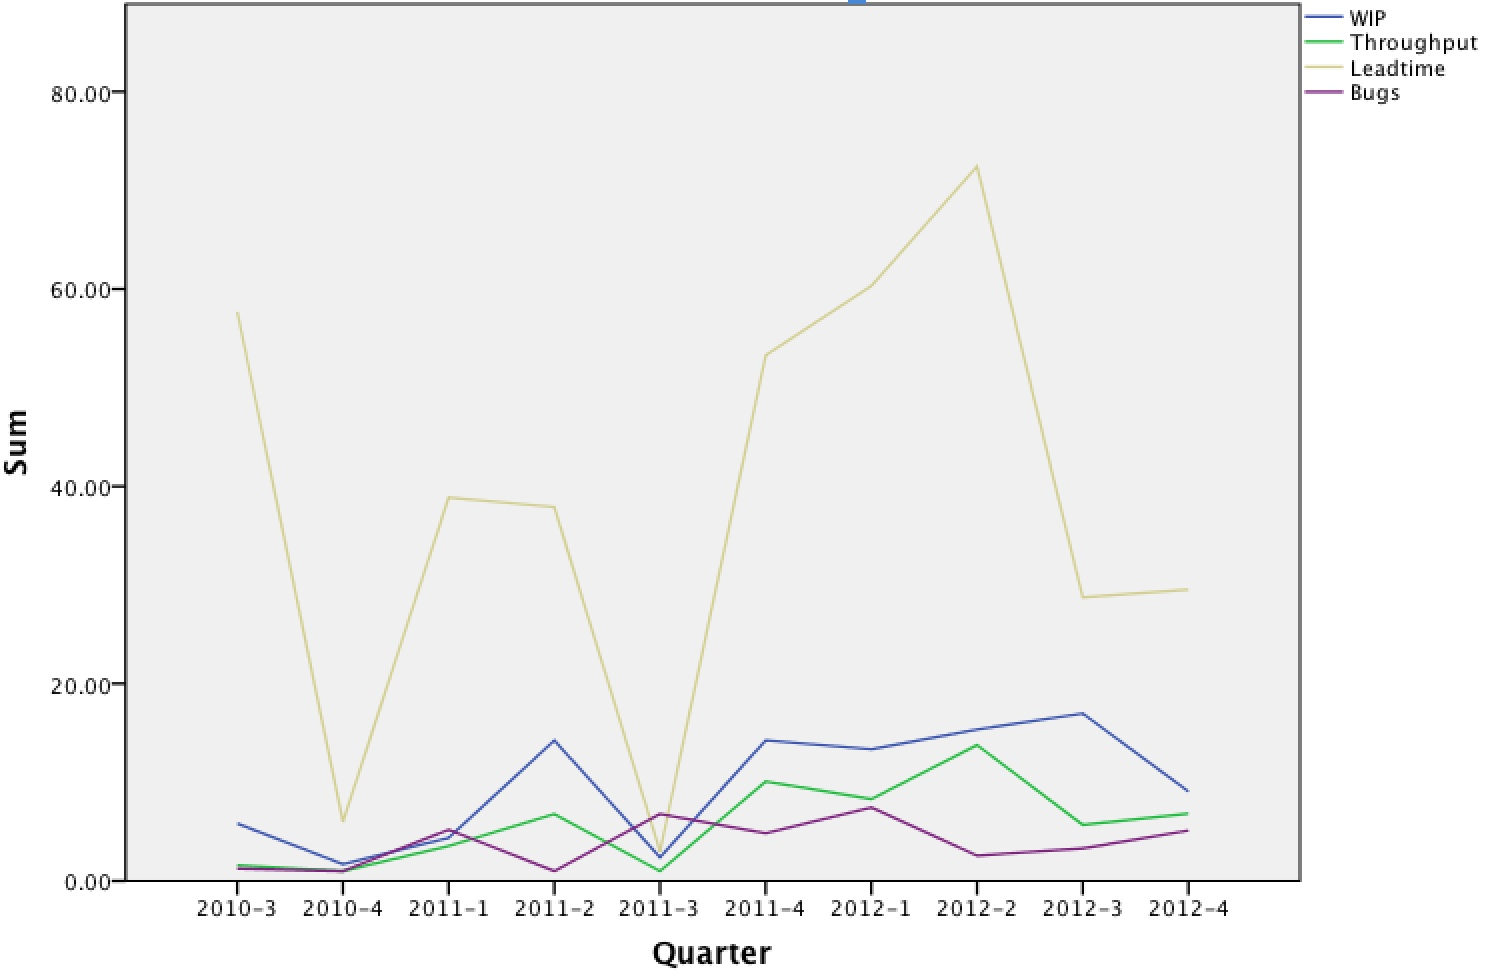
\includegraphics[scale=0.8]{Picture/360/360_WIP_TP_BUGS_LT.jpg}
\caption{WIP, Throughput, Lead time and Bugs for 360 per quarter}
\label{360pq} %% 360 per quarter
\end{figure}
\newpage

In figure \ref{Frontendpq} the average WIP, Throughput, Lead time and Bugs per quarter for team Frontend are shown
\begin{figure}[!htbp]
\centering
\hspace*{-1.2in}
\includegraphics[scale=0.7]{Picture/Frontend/Frontend-WIP-TP-LT-BUGS.jpg}
\caption{WIP, Throughput, Lead time and Bugs for Frontend per quarter}
\label{Frontendpq} %% fronted per quarter
\end{figure}
\newpage

In figure \ref{Kryptonpq} the average WIP, Throughput, Lead time and Bugs per quarter for team Krypton are shown
\begin{figure}[!htbp]
\centering
\hspace*{-1.8in}
\includegraphics[scale=0.8]{Picture/Krypton/Krypton-WIP-TP-BUGS-LT.jpg}
\caption{WIP, Throughput, Lead time and Bugs for Krypton per quarter}
\label{Kryptonpq} %% fronted per quarter
\end{figure}
\newpage


In figure \ref{Neonpq} the average WIP, Throughput, Lead time and Bugs per quarter for team Neon are shown
\begin{figure}[!htbp]
\centering
\hspace*{-1.2in}
\includegraphics[scale=1.5]{Picture/Neon/Neon-WIP-TP-BUGS-LT.jpg}
\caption{WIP, Throughput, Lead time and Bugs for Neon per quarter}
\label{Neonpq} %% fronted per quarter
\end{figure}


\chapter*{\centerline{Til Dag}}


\section {360}



  
\begin{table}[htbp]
  \centering
  \begin{adjustwidth}{-2cm}{}
  \scalebox{0.38}{
  \begin{tabular}{ | l | l | l | l | l | l | l | l | l | l | l | l | l | l | l | l | l | }
\hline
Correlations &  &  &  &  &  &  &  &  &  &  &  &  &  &  &  &  \\ \hline
	 &  & Bugs & Throughput & WIP & Churn & TP\_Feature & Churn\_Bugs & Leadtime\_Union & Churn\_Union & Churn\_feature & TP\_bugs & Average\_Days\_Backlog & Bugs\_churn\_average & Average\_ft\_churn & Precent\_bugs\_fininshed & Churn\_Average \\ \hline
	Bugs & Pearson Correlation & 1 & .945** & .753* & .992** & -0.328 & .813** & -0.240 & 0.433 & .730* & .984** & 0.377 & 0.581 & 0.119 & 0.543 & 0.622\\ \hline
	 & Sig. (2-tailed) &  & 0 & 0.012 & 0 & 0.354 & 0.004 & 0.505 & 0.212 & 0.026 & 0 & 0.282 & 0.078 & 0.744 & 0.104 & 0.055\\ \hline
	 & N & 10 & 10 & 10 & 10 & 10 & 10 & 10 & 10 & 9 & 10 & 10 & 10 & 10 & 10 & 10 \\ \hline
	Throughput & Pearson Correlation & .945** & 1 & .816** & .962** & -0.340 & .776** & -0.177 & 0.399 & .736* & .940** & 0.274 & 0.626 & 0.030 & 0.420 & .638* \\ \hline
	 & Sig. (2-tailed) & 0 &  & 0.004 & 0 & 0.336 & 0.008 & 0.624 & 0.253 & 0.024 & 0 & 0.443 & 0.053 & 0.934 & 0.227 & 0.047\\ \hline
	 & N & 10 & 10 & 10 & 10 & 10 & 10 & 10 & 10 & 9 & 10 & 10 & 10 & 10 & 10 & 10 \\ \hline
	WIP & Pearson Correlation & .753* & .816** & 1 & .738* & -0.441 & .708* & -0.336 & 0.365 & 0.467 & .800** & 0.397 & 0.430 & 0.243 & 0.495 & 0.478\\ \hline
	 & Sig. (2-tailed) & 0.012 & 0.004 &  & 0.015 & 0.202 & 0.022 & 0.342 & 0.299 & 0.205 & 0.005 & 0.255 & 0.215 & 0.498 & 0.146 & 0.163\\ \hline
	 & N & 10 & 10 & 10 & 10 & 10 & 10 & 10 & 10 & 9 & 10 & 10 & 10 & 10 & 10 & 10 \\ \hline
	Churn & Pearson Correlation & .992** & .962** & .738* & 1 & -0.317 & .804** & -0.203 & 0.372 & .741* & .974** & 0.349 & 0.581 & 0.087 & 0.475 & 0.617\\ \hline
	 & Sig. (2-tailed) & 0 & 0 & 0.015 &  & 0.372 & 0.005 & 0.574 & 0.289 & 0.022 & 0 & 0.323 & 0.078 & 0.811 & 0.165 & 0.057\\ \hline
	 & N & 10 & 10 & 10 & 10 & 10 & 10 & 10 & 10 & 9 & 10 & 10 & 10 & 10 & 10 & 10 \\ \hline
	TP\_Feature & Pearson Correlation & -0.328 & -0.340 & -0.441 & -0.317 & 1 & -0.419 & 0.376 & -0.460 & -0.208 & -0.360 & 0.097 & -0.171 & -0.295 & -.795** & -0.223\\ \hline
	 & Sig. (2-tailed) & 0.354 & 0.336 & 0.202 & 0.372 &  & 0.228 & 0.284 & 0.181 & 0.591 & 0.307 & 0.789 & 0.637 & 0.408 & 0.006 & 0.536\\ \hline
	 & N & 10 & 10 & 10 & 10 & 10 & 10 & 10 & 10 & 9 & 10 & 10 & 10 & 10 & 10 & 10 \\ \hline
	Churn\_Bugs & Pearson Correlation & .813** & .776** & .708* & .804** & -0.419 & 1 & -0.126 & 0.516 & 0.597 & .884** & .700* & 0.560 & 0.523 & 0.551 & .665* \\ \hline
	 & Sig. (2-tailed) & 0.004 & 0.008 & 0.022 & 0.005 & 0.228 &  & 0.729 & 0.127 & 0.090 & 0.001 & 0.024 & 0.092 & 0.121 & 0.099 & 0.036\\ \hline
	 & N & 10 & 10 & 10 & 10 & 10 & 10 & 10 & 10 & 9 & 10 & 10 & 10 & 10 & 10 & 10 \\ \hline
	Leadtime\_Union & Pearson Correlation & -0.240 & -0.177 & -0.336 & -0.203 & 0.376 & -0.126 & 1 & -0.060 & 0.138 & -0.280 & -0.012 & -0.003 & 0.158 & -0.598 & 0.059\\ \hline
	 & Sig. (2-tailed) & 0.505 & 0.624 & 0.342 & 0.574 & 0.284 & 0.729 &  & 0.868 & 0.724 & 0.433 & 0.974 & 0.994 & 0.663 & 0.068 & 0.871\\ \hline
	 & N & 10 & 10 & 10 & 10 & 10 & 10 & 10 & 10 & 9 & 10 & 10 & 10 & 10 & 10 & 10 \\ \hline
	Churn\_Union & Pearson Correlation & 0.433 & 0.399 & 0.365 & 0.372 & -0.460 & 0.516 & -0.060 & 1 & 0.202 & 0.466 & 0.231 & 0.146 & 0.410 & .634* & 0.198\\ \hline
	 & Sig. (2-tailed) & 0.212 & 0.253 & 0.299 & 0.289 & 0.181 & 0.127 & 0.868 &  & 0.603 & 0.175 & 0.522 & 0.687 & 0.239 & 0.049 & 0.584\\ \hline
	 & N & 10 & 10 & 10 & 10 & 10 & 10 & 10 & 10 & 9 & 10 & 10 & 10 & 10 & 10 & 10 \\ \hline
	Churn\_feature & Pearson Correlation & .730* & .736* & 0.467 & .741* & -0.208 & 0.597 & 0.138 & 0.202 & 1 & .681* & 0.073 & .924** & 0.008 & 0.362 & .947** \\ \hline
	 & Sig. (2-tailed) & 0.026 & 0.024 & 0.205 & 0.022 & 0.591 & 0.090 & 0.724 & 0.603 &  & 0.044 & 0.852 & 0 & 0.984 & 0.338 & 0\\ \hline
	 & N & 9 & 9 & 9 & 9 & 9 & 9 & 9 & 9 & 9 & 9 & 9 & 9 & 9 & 9 & 9 \\ \hline
	TP\_bugs & Pearson Correlation & .984** & .940** & .800** & .974** & -0.360 & .884** & -0.280 & 0.466 & .681* & 1 & 0.494 & 0.574 & 0.192 & 0.568 & 0.620\\ \hline
	 & Sig. (2-tailed) & 0 & 0 & 0.005 & 0 & 0.307 & 0.001 & 0.433 & 0.175 & 0.044 &  & 0.146 & 0.083 & 0.596 & 0.087 & 0.056\\ \hline
	 & N & 10 & 10 & 10 & 10 & 10 & 10 & 10 & 10 & 9 & 10 & 10 & 10 & 10 & 10 & 10 \\ \hline
	Average\_Days\_Backlog & Pearson Correlation & 0.377 & 0.274 & 0.397 & 0.349 & 0.097 & .700* & -0.012 & 0.231 & 0.073 & 0.494 & 1 & 0.101 & 0.595 & 0.130 & 0.217\\ \hline
	 & Sig. (2-tailed) & 0.282 & 0.443 & 0.255 & 0.323 & 0.789 & 0.024 & 0.974 & 0.522 & 0.852 & 0.146 &  & 0.782 & 0.070 & 0.721 & 0.548\\ \hline
	 & N & 10 & 10 & 10 & 10 & 10 & 10 & 10 & 10 & 9 & 10 & 10 & 10 & 10 & 10 & 10 \\ \hline
	Bugs\_churn\_average & Pearson Correlation & 0.581 & 0.626 & 0.430 & 0.581 & -0.171 & 0.560 & -0.003 & 0.146 & .924** & 0.574 & 0.101 & 1 & -0.127 & 0.322 & .973** \\ \hline
	 & Sig. (2-tailed) & 0.078 & 0.053 & 0.215 & 0.078 & 0.637 & 0.092 & 0.994 & 0.687 & 0 & 0.083 & 0.782 &  & 0.726 & 0.365 & 0\\ \hline
	 & N & 10 & 10 & 10 & 10 & 10 & 10 & 10 & 10 & 9 & 10 & 10 & 10 & 10 & 10 & 10 \\ \hline
	Average\_ft\_churn & Pearson Correlation & 0.119 & 0.030 & 0.243 & 0.087 & -0.295 & 0.523 & 0.158 & 0.410 & 0.008 & 0.192 & 0.595 & -0.127 & 1 & 0.291 & 0.088\\ \hline
	 & Sig. (2-tailed) & 0.744 & 0.934 & 0.498 & 0.811 & 0.408 & 0.121 & 0.663 & 0.239 & 0.984 & 0.596 & 0.070 & 0.726 &  & 0.415 & 0.808\\ \hline
	 & N & 10 & 10 & 10 & 10 & 10 & 10 & 10 & 10 & 9 & 10 & 10 & 10 & 10 & 10 & 10 \\ \hline
	Precent\_bugs\_fininshed & Pearson Correlation & 0.543 & 0.420 & 0.495 & 0.475 & -.795** & 0.551 & -0.598 & .634* & 0.362 & 0.568 & 0.130 & 0.322 & 0.291 & 1 & 0.369\\ \hline
	 & Sig. (2-tailed) & 0.104 & 0.227 & 0.146 & 0.165 & 0.006 & 0.099 & 0.068 & 0.049 & 0.338 & 0.087 & 0.721 & 0.365 & 0.415 &  & 0.294\\ \hline
	 & N & 10 & 10 & 10 & 10 & 10 & 10 & 10 & 10 & 9 & 10 & 10 & 10 & 10 & 10 & 10 \\ \hline
	Churn\_Average & Pearson Correlation & 0.622 & .638* & 0.478 & 0.617 & -0.223 & .665* & 0.059 & 0.198 & .947** & 0.620 & 0.217 & .973** & 0.088 & 0.369 & 1 \\ \hline
	 & Sig. (2-tailed) & 0.055 & 0.047 & 0.163 & 0.057 & 0.536 & 0.036 & 0.871 & 0.584 & 0 & 0.056 & 0.548 & 0 & 0.808 & 0.294 &  \\ \hline
	 & N & 10 & 10 & 10 & 10 & 10 & 10 & 10 & 10 & 9 & 10 & 10 & 10 & 10 & 10 & 10 \\ \hline
	 \end{tabular}
 }
  \centerline{  ** Correlation is significant at the 0.01 level (2-tailed).}
    \centerline {* Correlation is significant at the 0.05 level (2-tailed).}
      \caption{360 - Correlation}
  \label{tab:addlabelSwag}%
 \end{adjustwidth}
\end{table}%
\begin{table}[!htbp]
\centering
  \begin{adjustwidth}{-1cm}{}
     \scalebox{0.75}{
\begin{tabular}{ | l | l | l | l | l | }
\hline
	 &  &  &  &  \\ \hline
	Team & Quarter &  & Churn & Leadtime \\ \hline
	360 & 2010-3 & N & 11 & 11 \\ \hline
	 &  & Mean & 17 & 3.55 \\ \hline
	 &  & Median & 11 & 3 \\ \hline
	 &  & Std. Deviation & 18.93 & 2.50 \\ \hline
	 &  & Maximum & 60 & 8 \\ \hline
	 &  & Minimum & 0 & 1 \\ \hline
	 &  &  &  &  \\ \hline
	 & 2010-4 & N & 3 & 3 \\ \hline
	 &  & Mean & 0.67 & 1.67 \\ \hline
	 &  & Median & 1 & 2 \\ \hline
	 &  & Std. Deviation & 0.57 & 0.57 \\ \hline
	 &  & Maximum & 1 & 2 \\ \hline
	 &  & Minimum & 0 & 1 \\ \hline
	 &  & N & 136 & 136 \\ \hline
	 & 2011-2 & Mean & 14.4 & 2.7 \\ \hline
	 &  & Median & 3 & 2 \\ \hline
	 &  & Std. Deviation & 21.51 & 1.85 \\ \hline
	 &  & Maximum & 83 & 8 \\ \hline
	 &  & Minimum & 0 & 1 \\ \hline
	 &  & N & 48 & 48 \\ \hline
	 & 2011-3 & Mean & 1.67 & 3.06 \\ \hline
	 &  & Median & 0 & 2.5 \\ \hline
	 &  & Std. Deviation & 7.71 & 2.13 \\ \hline
	 &  & Maximum & 50 & 8 \\ \hline
	 &  & Minimum & 0 & 1 \\ \hline
	 &  & N & 156 & 156 \\ \hline
	 & 2011-4 & Mean & 14.81 & 2.25 \\ \hline
	 &  & Median & 6.5 & 2 \\ \hline
	 &  & Std. Deviation & 19.90 & 1.53 \\ \hline
	 &  & Maximum & 86 & 8 \\ \hline
	 &  & Minimum & 0 & 1 \\ \hline
	 &  & N & 157 & 157 \\ \hline
	 & 2012-1 & Mean & 9.47 & 2.68 \\ \hline
	 &  & Median & 0 & 2 \\ \hline
	 &  & Std. Deviation & 19.54 & 1.758 \\ \hline
	 &  & Maximum & 86 & 8 \\ \hline
	 &  & Minimum & 0 & 1 \\ \hline
	 &  & N & 238 & 238 \\ \hline
	 & 2012-2 & Mean & 10.11 & 2.78 \\ \hline
	 &  & Median & 0 & 2 \\ \hline
	 &  & Std. Deviation & 18.50 & 1.597 \\ \hline
	 &  & Maximum & 83 & 8 \\ \hline
	 &  & Minimum & 0 & 1 \\ \hline
	 &  & N & 53 & 53 \\ \hline
	 & 2012-3 & Mean & 3.02 & 1.68 \\ \hline
	 &  & Median & 0 & 1 \\ \hline
	 &  & Std. Deviation & 9.61 & 1.18\\ \hline
	 &  & Maximum & 53 & 7 \\ \hline
	 &  & Minimum & 0 & 1 \\ \hline
	 &  & N & 26 & 26 \\ \hline
	 & 2012-4 & Mean & 21.42 & 2.08 \\ \hline
	 &  & Median & 14.5 & 2 \\ \hline
	 &  & Std. Deviation & 20.54 & 1.16 \\ \hline
	 &  & Maximum & 67 & 5 \\ \hline
	 &  & Minimum & 1 & 1 \\ \hline
	 &  & N & 902 & 902 \\ \hline
	 & Total & Mean & 10.14 & 2.7 \\ \hline
	 &  & Median & 0 & 2 \\ \hline
	 &  & Std. Deviation & 18.55 & 1.798 \\ \hline
	 &  & Maximum & 86 & 8 \\ \hline
	 &  & Minimum & 0 & 1 \\ \hline
\end{tabular}
}
\caption{Descriptive statistic  - Lead-time and churn - 360}
\end{adjustwidth}
 \end{table}%
 
	

 
%%%%%%%%%%%%%%%%%
\section*{Frontend} 
 \begin{table}[!htbp]
  \centering
    \begin{adjustwidth}{-2.5cm}{}
    \scalebox{0.38}{
    \begin{tabular}{ | l | l | l | l | l | l | l | l | l | l | l | l | l | l | l | l | l | }
\hline
	Correlations &  &  &  &  &  &  &  &  &  &  &  &  &  &  &  &  \\ \hline
	 &  & WIP & Throughput & Bugs & Churn & TP\_feature & Churn\_Bugs & Churn\_union & Leadtime\_union & Churn\_feature & Tp\_bugs & Average\_Days\_Backlog\_Bugs & Bugs\_Churn\_average & Churn\_feature\_Average & Precent\_bugs\_fininshed & Churn\_Average \\ \hline
	WIP & Pearson Correlation & 1 & 0.491 & 0.278 & -0.446 & 0.380 & -0.446 & 0.316 & 0.096 & 0.362 & 0.508 & -0.178 & 0.257 & 0.337 & 0.367 & 0.223\\ \hline
	 & Sig. (2-tailed) &  & 0.150 & 0.436 & 0.196 & 0.279 & 0.196 & 0.373 & 0.791 & 0.304 & 0.134 & 0.622 & 0.473 & 0.341 & 0.297 & 0.537\\ \hline
	 & N & 10 & 10 & 10 & 10 & 10 & 10 & 10 & 10 & 10 & 10 & 10 & 10 & 10 & 10 & 10 \\ \hline
	Throughput & Pearson Correlation & 0.491 & 1 & .773** & -0.036 & .741* & 0.217 & -0.494 & -0.539 & -0.433 & .758* & 0.055 & 0.259 & -0.609 & .745* & -0.575\\ \hline
	 & Sig. (2-tailed) & 0.150 &  & 0.009 & 0.921 & 0.014 & 0.548 & 0.147 & 0.108 & 0.212 & 0.011 & 0.879 & 0.470 & 0.062 & 0.013 & 0.082\\ \hline
	 & N & 10 & 10 & 10 & 10 & 10 & 10 & 10 & 10 & 10 & 10 & 10 & 10 & 10 & 10 & 10 \\ \hline
	Bugs & Pearson Correlation & 0.278 & .773** & 1 & 0.259 & 0.534 & 0.398 & -0.555 & -0.581 & -0.478 & 0.271 & 0.005 & 0.296 & -0.571 & 0.498 & -0.624\\ \hline
	 & Sig. (2-tailed) & 0.436 & 0.009 &  & 0.471 & 0.111 & 0.254 & 0.096 & 0.078 & 0.162 & 0.449 & 0.988 & 0.407 & 0.085 & 0.143 & 0.054\\ \hline
	 & N & 10 & 10 & 10 & 10 & 10 & 10 & 10 & 10 & 10 & 10 & 10 & 10 & 10 & 10 & 10 \\ \hline
	Churn & Pearson Correlation & -0.446 & -0.036 & 0.259 & 1 & -0.219 & .791** & -0.522 & -0.449 & -0.517 & -0.110 & -0.174 & 0.172 & -0.485 & -0.014 & -0.471\\ \hline
	 & Sig. (2-tailed) & 0.196 & 0.921 & 0.471 &  & 0.543 & 0.006 & 0.122 & 0.192 & 0.126 & 0.762 & 0.631 & 0.634 & 0.155 & 0.970 & 0.170\\ \hline
	 & N & 10 & 10 & 10 & 10 & 10 & 10 & 10 & 10 & 10 & 10 & 10 & 10 & 10 & 10 & 10 \\ \hline
	TP\_feature & Pearson Correlation & 0.380 & .741* & 0.534 & -0.219 & 1 & 0.214 & -0.244 & -0.312 & -0.026 & 0.427 & -0.256 & -0.007 & -0.294 & .640* & -0.319\\ \hline
	 & Sig. (2-tailed) & 0.279 & 0.014 & 0.111 & 0.543 &  & 0.553 & 0.497 & 0.381 & 0.943 & 0.219 & 0.475 & 0.984 & 0.409 & 0.046 & 0.369\\ \hline
	 & N & 10 & 10 & 10 & 10 & 10 & 10 & 10 & 10 & 10 & 10 & 10 & 10 & 10 & 10 & 10 \\ \hline
	Churn\_Bugs & Pearson Correlation & -0.446 & 0.217 & 0.398 & .791** & 0.214 & 1 & -.707* & -.771** & -0.460 & 0.040 & -0.378 & -0.035 & -0.590 & 0.388 & -.689* \\ \hline
	 & Sig. (2-tailed) & 0.196 & 0.548 & 0.254 & 0.006 & 0.553 &  & 0.022 & 0.009 & 0.181 & 0.912 & 0.282 & 0.924 & 0.073 & 0.267 & 0.027\\ \hline
	 & N & 10 & 10 & 10 & 10 & 10 & 10 & 10 & 10 & 10 & 10 & 10 & 10 & 10 & 10 & 10 \\ \hline
	Churn\_union & Pearson Correlation & 0.316 & -0.494 & -0.555 & -0.522 & -0.244 & -.707* & 1 & .704* & .844** & -0.368 & -0.139 & 0.152 & .841** & -0.312 & .981** \\ \hline
	 & Sig. (2-tailed) & 0.373 & 0.147 & 0.096 & 0.122 & 0.497 & 0.022 &  & 0.023 & 0.002 & 0.296 & 0.702 & 0.674 & 0.002 & 0.379 & 0\\ \hline
	 & N & 10 & 10 & 10 & 10 & 10 & 10 & 10 & 10 & 10 & 10 & 10 & 10 & 10 & 10 & 10 \\ \hline
	Leadtime\_union & Pearson Correlation & 0.096 & -0.539 & -0.581 & -0.449 & -0.312 & -.771** & .704* & 1 & 0.492 & -0.301 & 0.327 & -0.227 & 0.631 & -.697* & .766** \\ \hline
	 & Sig. (2-tailed) & 0.791 & 0.108 & 0.078 & 0.192 & 0.381 & 0.009 & 0.023 &  & 0.148 & 0.398 & 0.357 & 0.528 & 0.050 & 0.025 & 0.010\\ \hline
	 & N & 10 & 10 & 10 & 10 & 10 & 10 & 10 & 10 & 10 & 10 & 10 & 10 & 10 & 10 & 10 \\ \hline
	Churn\_feature & Pearson Correlation & 0.362 & -0.433 & -0.478 & -0.517 & -0.026 & -0.460 & .844** & 0.492 & 1 & -0.314 & -0.358 & -0.201 & .921** & -0.172 & .842** \\ \hline
	 & Sig. (2-tailed) & 0.304 & 0.212 & 0.162 & 0.126 & 0.943 & 0.181 & 0.002 & 0.148 &  & 0.377 & 0.310 & 0.579 & 0 & 0.635 & 0.002\\ \hline
	 & N & 10 & 10 & 10 & 10 & 10 & 10 & 10 & 10 & 10 & 10 & 10 & 10 & 10 & 10 & 10 \\ \hline
	Tp\_bugs & Pearson Correlation & 0.508 & .758* & 0.271 & -0.110 & 0.427 & 0.040 & -0.368 & -0.301 & -0.314 & 1 & 0.096 & 0.034 & -0.393 & 0.622 & -0.406\\ \hline
	 & Sig. (2-tailed) & 0.134 & 0.011 & 0.449 & 0.762 & 0.219 & 0.912 & 0.296 & 0.398 & 0.377 &  & 0.792 & 0.926 & 0.261 & 0.055 & 0.245\\ \hline
	 & N & 10 & 10 & 10 & 10 & 10 & 10 & 10 & 10 & 10 & 10 & 10 & 10 & 10 & 10 & 10 \\ \hline
	Average\_Days\_Backlog\_Bugs & Pearson Correlation & -0.178 & 0.055 & 0.005 & -0.174 & -0.256 & -0.378 & -0.139 & 0.327 & -0.358 & 0.096 & 1 & -0.267 & -0.272 & -0.489 & -0.035\\ \hline
	 & Sig. (2-tailed) & 0.622 & 0.879 & 0.988 & 0.631 & 0.475 & 0.282 & 0.702 & 0.357 & 0.310 & 0.792 &  & 0.456 & 0.446 & 0.151 & 0.925\\ \hline
	 & N & 10 & 10 & 10 & 10 & 10 & 10 & 10 & 10 & 10 & 10 & 10 & 10 & 10 & 10 & 10 \\ \hline
	Bugs\_Churn\_average & Pearson Correlation & 0.257 & 0.259 & 0.296 & 0.172 & -0.007 & -0.035 & 0.152 & -0.227 & -0.201 & 0.034 & -0.267 & 1 & -0.197 & 0.371 & 0.016\\ \hline
	 & Sig. (2-tailed) & 0.473 & 0.470 & 0.407 & 0.634 & 0.984 & 0.924 & 0.674 & 0.528 & 0.579 & 0.926 & 0.456 &  & 0.585 & 0.291 & 0.966\\ \hline
	 & N & 10 & 10 & 10 & 10 & 10 & 10 & 10 & 10 & 10 & 10 & 10 & 10 & 10 & 10 & 10 \\ \hline
	Churn\_feature\_Average & Pearson Correlation & 0.337 & -0.609 & -0.571 & -0.485 & -0.294 & -0.590 & .841** & 0.631 & .921** & -0.393 & -0.272 & -0.197 & 1 & -0.389 & .846** \\ \hline
	 & Sig. (2-tailed) & 0.341 & 0.062 & 0.085 & 0.155 & 0.409 & 0.073 & 0.002 & 0.050 & 0 & 0.261 & 0.446 & 0.585 &  & 0.267 & 0.002\\ \hline
	 & N & 10 & 10 & 10 & 10 & 10 & 10 & 10 & 10 & 10 & 10 & 10 & 10 & 10 & 10 & 10 \\ \hline
	Precent\_bugs\_fininshed & Pearson Correlation & 0.367 & .745* & 0.498 & -0.014 & .640* & 0.388 & -0.312 & -.697* & -0.172 & 0.622 & -0.489 & 0.371 & -0.389 & 1 & -0.445\\ \hline
	 & Sig. (2-tailed) & 0.297 & 0.013 & 0.143 & 0.970 & 0.046 & 0.267 & 0.379 & 0.025 & 0.635 & 0.055 & 0.151 & 0.291 & 0.267 &  & 0.197\\ \hline
	 & N & 10 & 10 & 10 & 10 & 10 & 10 & 10 & 10 & 10 & 10 & 10 & 10 & 10 & 10 & 10 \\ \hline
	Churn\_Average & Pearson Correlation & 0.223 & -0.575 & -0.624 & -0.471 & -0.319 & -.689* & .981** & .766** & .842** & -0.406 & -0.035 & 0.016 & .846** & -0.445 & 1 \\ \hline
	 & Sig. (2-tailed) & 0.537 & 0.082 & 0.054 & 0.170 & 0.369 & 0.027 & 0 & 0.010 & 0.002 & 0.245 & 0.925 & 0.966 & 0.002 & 0.197 &  \\ \hline
	 & N & 10 & 10 & 10 & 10 & 10 & 10 & 10 & 10 & 10 & 10 & 10 & 10 & 10 & 10 & 10 \\ \hline
\end{tabular}
    }
       \centerline{  ** Correlation is significant at the 0.01 level (2-tailed).}
    \centerline {* Correlation is significant at the 0.05 level (2-tailed).}
      \caption{Frontend Correlation}
   \end{adjustwidth}
\end{table}%

\begin{table}[!htbp]
\centering
  \begin{adjustwidth}{-1cm}{}
     \scalebox{0.75}{
\begin{tabular}{ | l | l | l | l | l | } 
\hline
	Team & Quarter &  & Leadtime & Churn \\ \hline
	Frontend & 2010-3 & N & 58 & 58 \\ \hline
	 &  & Mean & 7.43 & 127.93 \\ \hline
	 &  & Median & 6 & 53.5 \\ \hline
	 &  & Std. Deviation & 5.567 & 187.011 \\ \hline
	 &  & Maximum & 22 & 1072 \\ \hline
	 &  & Minimum & 1 & 0 \\ \hline
	 & 2010-4 & N & 130 & 130 \\ \hline
	 &  & Mean & 10.32 & 158.72 \\ \hline
	 &  & Median & 4 & 14 \\ \hline
	 &  & Std. Deviation & 15.30 & 444.805 \\ \hline
	 &  & Maximum & 78 & 4308 \\ \hline
	 &  & Minimum & 1 & 0 \\ \hline
	 & 2011-1 & N & 95 & 95 \\ \hline
	 &  & Mean & 28.01 & 566.73 \\ \hline
	 &  & Median & 11 & 47 \\ \hline
	 &  & Std. Deviation & 52.183 & 3696.125 \\ \hline
	 &  & Maximum & 434 & 35917 \\ \hline
	 &  & Minimum & 1 & 0 \\ \hline
	 & 2011-2 & N & 132 & 132 \\ \hline
	 &  & Mean & 12.17 & 496.8 \\ \hline
	 &  & Median & 5 & 19 \\ \hline
	 &  & Std. Deviation & 23.548 & 3240.172 \\ \hline
	 &  & Maximum & 184 & 35956 \\ \hline
	 &  & Minimum & 1 & 0 \\ \hline
	 & 2011-3 & N & 146 & 146 \\ \hline
	 &  & Mean & 10.66 & 174.07 \\ \hline
	 &  & Median & 6 & 14 \\ \hline
	 &  & Std. Deviation & 12.577 & 655.578 \\ \hline
	 &  & Maximum & 79 & 5650 \\ \hline
	 &  & Minimum & 1 & 0 \\ \hline
	 & 2011-4 & N & 167 & 167 \\ \hline
	 &  & Mean & 9.85 & 110.98 \\ \hline
	 &  & Median & 7 & 3 \\ \hline
	 &  & Std. Deviation & 10.9 & 480.32 \\ \hline
	 &  & Maximum & 62 & 5672 \\ \hline
	 &  & Minimum & 1 & 0 \\ \hline
	 & 2012-1 & N & 188 & 188 \\ \hline
	 &  & Mean & 13.9 & 118.64 \\ \hline
	 &  & Median & 8 & 5.5 \\ \hline
	 &  & Std. Deviation & 21.92 & 568.03 \\ \hline
	 &  & Maximum & 150 & 7565 \\ \hline
	 &  & Minimum & 1 & 0 \\ \hline
	 & 2012-2 & N & 77 & 77 \\ \hline
	 &  & Mean & 22.53 & 849.42 \\ \hline
	 &  & Median & 17 & 15 \\ \hline
	 &  & Std. Deviation & 25.52 & 3575.50 \\ \hline
	 &  & Maximum & 106 & 27170 \\ \hline
	 &  & Minimum & 1 & 0 \\ \hline
	 & 2012-3 & N & 93 & 93 \\ \hline
	 &  & Mean & 13.76 & 458.92 \\ \hline
	 &  & Median & 8 & 25 \\ \hline
	 &  & Std. Deviation & 18.023 & 1272.32 \\ \hline
	 &  & Maximum & 107 & 8600 \\ \hline
	 &  & Minimum & 1 & 0 \\ \hline
	 & 2012-4 & N & 82 & 82 \\ \hline
	 &  & Mean & 8.8007 & 428.67 \\ \hline
	 &  & Median & 4 & 54 \\ \hline
	 &  & Std. Deviation & 14.978& 1178.471 \\ \hline
	 &  & Maximum & 83 & 9368 \\ \hline
	 &  & Minimum & 1 & 0 \\ \hline
	 & Total & N & 1168 & 1168 \\ \hline
	 &  & Mean & 13.35 & 305.62 \\ \hline
	 &  & Median & 7 & 15 \\ \hline
	 &  & Std. Deviation & 23.15 & 1883.16 \\ \hline
	 &  & Maximum & 434 & 35956 \\ \hline
	 &  & Minimum & 1 & 0 \\ \hline
\end{tabular}
}
\caption{Descriptive statistic  - Lead-time and churn - Frontend}
\end{adjustwidth}
 \end{table}%
 

 

 \begin{table}[!htbp]
\begin{tabular}{ | l | l | l | l | l | l | l | l | }
\hline
TeamName & Quarter & N & Mean & Median & Std. Deviation & Maximum & Minimum \\ \hline
Frontend & 2010-3 & 14 & 2.79 & 2 & 2.91 & 12 & 1 \\ \hline
	 & 2010-4 & 39 & 2 & 1 & 1.53 & 8 & 1 \\ \hline
	 & 2011-1 & 20 & 1.85 & 1 & 1.226 & 5 & 1 \\ \hline
	 & 2011-2 & 29 & 2.86 & 2 & 3.21 & 16 & 1 \\ \hline
	 & 2011-3 & 37 & 2.41 & 2 & 1.93 & 10 & 1 \\ \hline
	 & 2011-4 & 35 & 2.89 & 1 & 5.02 & 30 & 1 \\ \hline
	 & 2012-1 & 39 & 3.56 & 2 & 3.90& 23 & 1 \\ \hline
	 & 2012-2 & 31 & 1.81 & 1 & 1.4 & 7 & 1 \\ \hline
	 & 2012-3 & 24 & 2.54 & 2 & 1.79 & 7 & 1 \\ \hline
	 & 2012-4 & 14 & 2.86 & 2 & 1.79 & 7 & 1 \\ \hline
	 & Total & 282 & 2.56 & 2 & 2.895 & 30 & 1 \\ \hline
	 	 \end{tabular}
  	  \caption{Frontend - Descriptive statistic - Bugs }%
\end{table}

 \begin{table}[!htbp]
\begin{tabular}{ | l | l | l | l | l | l | l | l | }
\hline
TeamName & Quarter & N & Mean & Median & Std. Deviation & Maximum & Minimum \\ \hline
Frontend & 2010-3 & 8 & 1.25 & 1 & 0.46 & 2 & 1 \\ \hline
	 & 2010-4 & 35 & 1.63 & 1 & 0.877 & 4 & 1 \\ \hline
	 & 2011-1 & 32 & 1.53 & 1 & 0.67& 3 & 1 \\ \hline
	 & 2011-2 & 31 & 1.74 & 2 & 0.89 & 4 & 1 \\ \hline
	 & 2011-3 & 31 & 1.97 & 2 & 1.25& 6 & 1 \\ \hline
	 & 2011-4 & 28 & 1.93 & 1 & 1.94& 11 & 1 \\ \hline
	 & 2012-1 & 22 & 2.18& 1 & 2.01 & 7 & 1 \\ \hline
	 & 2012-2 & 23 & 1.48 & 1 & 1.123 & 6 & 1 \\ \hline
	 & 2012-3 & 21 & 1.48 & 1 & 0.873 & 4 & 1 \\ \hline
	 & 2012-4 & 19 & 2.47 & 2 & 1.679 & 8 & 1 \\ \hline
	 & Total & 250 & 1.78 & 1 & 1.294 & 11 & 1 \\ \hline
 	 \end{tabular}
  	  \caption{Frontend - Descriptive statistic - TP feature }%
\end{table}

 \begin{table}[!htbp]
\begin{tabular}{ | l | l | l | l | l | l | l | l | }
\hline
TeamName & Quarter & N & Mean & Median & Std. Deviation & Maximum & Minimum \\ \hline
	Frontend & 2010-3 & 15 & 2 & 2 & 1.363 & 6 & 1 \\ \hline
	 & 2010-4 & 41 & 1.98 & 2 & 1.387 & 8 & 1 \\ \hline
	 & 2011-1 & 18 & 1.33 & 1 & 0.48 & 2 & 1 \\ \hline
	 & 2011-2 & 35 & 2.50 & 2 & 2.161 & 10 & 1 \\ \hline
	 & 2011-3 & 38 & 2.18 & 2 & 1.60 & 8 & 1 \\ \hline
	 & 2011-4 & 40 & 2.6 & 2 & 2.52 & 14 & 1 \\ \hline
	 & 2012-1 & 41 & 3.44 & 3 & 2.61 & 10 & 1 \\ \hline
	 & 2012-2 & 29 & 1.9 & 1 & 1.472 & 7 & 1 \\ \hline
	 & 2012-3 & 30 & 2.13 & 1.5 & 1.69 & 8 & 1 \\ \hline
	 & 2012-4 & 25 & 2.12 & 1 & 2.10 & 10 & 1 \\ \hline
	 & Total & 312 & 2.31 & 2 & 1.982 & 14 & 1 \\ \hline
 	 \end{tabular}
  	  \caption{Frontend - Descriptive statistic - TP bugs }%
\end{table}
%%%%%%%%%%%%%%

\section{Krypton}
\begin{table}[!htbp]
  \centering
   \begin{adjustwidth}{-2.5cm}{}
    \scalebox{0.38}{
    \begin{tabular}{|l|l|l|l|l|l|l|l|l|}
    \hline
      \begin{tabular}{ | l | l | l | l | l | l | l | l | l | l | l | l | l | l | l | l | l | }
\hline
	Correlations &  &  &  &  &  &  &  &  &  &  &  &  &  &  &  &  \\ \hline
	 &  & WIP & Throughput & Bugs & Churn & TP\_feature & Churn\_Bugs & Churn\_union & Leadtime\_union & Churn\_feature & Tp\_bugs & Average\_Days\_Backlog\_Bugs & Bugs\_Churn\_average & Churn\_feature\_Average & Precent\_bugs\_fininshed & Churn\_Average \\ \hline
	WIP & Pearson Correlation & 1 & 0.491 & 0.278 & -0.446 & 0.380 & -0.446 & 0.316 & 0.096 & 0.362 & 0.508 & -0.178 & 0.257 & 0.337 & 0.367 & 0.223\\ \hline
	 & Sig. (2-tailed) &  & 0.150 & 0.436 & 0.196 & 0.279 & 0.196 & 0.373 & 0.791 & 0.304 & 0.134 & 0.622 & 0.473 & 0.341 & 0.297 & 0.537\\ \hline
	 & N & 10 & 10 & 10 & 10 & 10 & 10 & 10 & 10 & 10 & 10 & 10 & 10 & 10 & 10 & 10 \\ \hline
	Throughput & Pearson Correlation & 0.491 & 1 & .773** & -0.036 & .741* & 0.217 & -0.494 & -0.539 & -0.433 & .758* & 0.055 & 0.259 & -0.609 & .745* & -0.575\\ \hline
	 & Sig. (2-tailed) & 0.150 &  & 0.009 & 0.921 & 0.014 & 0.548 & 0.147 & 0.108 & 0.212 & 0.011 & 0.879 & 0.470 & 0.062 & 0.013 & 0.082\\ \hline
	 & N & 10 & 10 & 10 & 10 & 10 & 10 & 10 & 10 & 10 & 10 & 10 & 10 & 10 & 10 & 10 \\ \hline
	Bugs & Pearson Correlation & 0.278 & .773** & 1 & 0.259 & 0.534 & 0.398 & -0.555 & -0.581 & -0.478 & 0.271 & 0.005 & 0.296 & -0.571 & 0.498 & -0.624\\ \hline
	 & Sig. (2-tailed) & 0.436 & 0.009 &  & 0.471 & 0.111 & 0.254 & 0.096 & 0.078 & 0.162 & 0.449 & 0.988 & 0.407 & 0.085 & 0.143 & 0.054\\ \hline
	 & N & 10 & 10 & 10 & 10 & 10 & 10 & 10 & 10 & 10 & 10 & 10 & 10 & 10 & 10 & 10 \\ \hline
	Churn & Pearson Correlation & -0.446 & -0.036 & 0.259 & 1 & -0.219 & .791** & -0.522 & -0.449 & -0.517 & -0.110 & -0.174 & 0.172 & -0.485 & -0.014 & -0.471\\ \hline
	 & Sig. (2-tailed) & 0.196 & 0.921 & 0.471 &  & 0.543 & 0.006 & 0.122 & 0.192 & 0.126 & 0.762 & 0.631 & 0.634 & 0.155 & 0.970 & 0.170\\ \hline
	 & N & 10 & 10 & 10 & 10 & 10 & 10 & 10 & 10 & 10 & 10 & 10 & 10 & 10 & 10 & 10 \\ \hline
	TP\_feature & Pearson Correlation & 0.380 & .741* & 0.534 & -0.219 & 1 & 0.214 & -0.244 & -0.312 & -0.026 & 0.427 & -0.256 & -0.007 & -0.294 & .640* & -0.319\\ \hline
	 & Sig. (2-tailed) & 0.279 & 0.014 & 0.111 & 0.543 &  & 0.553 & 0.497 & 0.381 & 0.943 & 0.219 & 0.475 & 0.984 & 0.409 & 0.046 & 0.369\\ \hline
	 & N & 10 & 10 & 10 & 10 & 10 & 10 & 10 & 10 & 10 & 10 & 10 & 10 & 10 & 10 & 10 \\ \hline
	Churn\_Bugs & Pearson Correlation & -0.446 & 0.217 & 0.398 & .791** & 0.214 & 1 & -.707* & -.771** & -0.460 & 0.040 & -0.378 & -0.035 & -0.590 & 0.388 & -.689* \\ \hline
	 & Sig. (2-tailed) & 0.196 & 0.548 & 0.254 & 0.006 & 0.553 &  & 0.022 & 0.009 & 0.181 & 0.912 & 0.282 & 0.924 & 0.073 & 0.267 & 0.027\\ \hline
	 & N & 10 & 10 & 10 & 10 & 10 & 10 & 10 & 10 & 10 & 10 & 10 & 10 & 10 & 10 & 10 \\ \hline
	Churn\_union & Pearson Correlation & 0.316 & -0.494 & -0.555 & -0.522 & -0.244 & -.707* & 1 & .704* & .844** & -0.368 & -0.139 & 0.152 & .841** & -0.312 & .981** \\ \hline
	 & Sig. (2-tailed) & 0.373 & 0.147 & 0.096 & 0.122 & 0.497 & 0.022 &  & 0.023 & 0.002 & 0.296 & 0.702 & 0.674 & 0.002 & 0.379 & 0\\ \hline
	 & N & 10 & 10 & 10 & 10 & 10 & 10 & 10 & 10 & 10 & 10 & 10 & 10 & 10 & 10 & 10 \\ \hline
	Leadtime\_union & Pearson Correlation & 0.096 & -0.539 & -0.581 & -0.449 & -0.312 & -.771** & .704* & 1 & 0.492 & -0.301 & 0.327 & -0.227 & 0.631 & -.697* & .766** \\ \hline
	 & Sig. (2-tailed) & 0.791 & 0.108 & 0.078 & 0.192 & 0.381 & 0.009 & 0.023 &  & 0.148 & 0.398 & 0.357 & 0.528 & 0.050 & 0.025 & 0.010\\ \hline
	 & N & 10 & 10 & 10 & 10 & 10 & 10 & 10 & 10 & 10 & 10 & 10 & 10 & 10 & 10 & 10 \\ \hline
	Churn\_feature & Pearson Correlation & 0.362 & -0.433 & -0.478 & -0.517 & -0.026 & -0.460 & .844** & 0.492 & 1 & -0.314 & -0.358 & -0.201 & .921** & -0.172 & .842** \\ \hline
	 & Sig. (2-tailed) & 0.304 & 0.212 & 0.162 & 0.126 & 0.943 & 0.181 & 0.002 & 0.148 &  & 0.377 & 0.310 & 0.579 & 0 & 0.635 & 0.002\\ \hline
	 & N & 10 & 10 & 10 & 10 & 10 & 10 & 10 & 10 & 10 & 10 & 10 & 10 & 10 & 10 & 10 \\ \hline
	Tp\_bugs & Pearson Correlation & 0.508 & .758* & 0.271 & -0.110 & 0.427 & 0.040 & -0.368 & -0.301 & -0.314 & 1 & 0.096 & 0.034 & -0.393 & 0.622 & -0.406\\ \hline
	 & Sig. (2-tailed) & 0.134 & 0.011 & 0.449 & 0.762 & 0.219 & 0.912 & 0.296 & 0.398 & 0.377 &  & 0.792 & 0.926 & 0.261 & 0.055 & 0.245\\ \hline
	 & N & 10 & 10 & 10 & 10 & 10 & 10 & 10 & 10 & 10 & 10 & 10 & 10 & 10 & 10 & 10 \\ \hline
	Average\_Days\_Backlog\_Bugs & Pearson Correlation & -0.178 & 0.055 & 0.005 & -0.174 & -0.256 & -0.378 & -0.139 & 0.327 & -0.358 & 0.096 & 1 & -0.267 & -0.272 & -0.489 & -0.035\\ \hline
	 & Sig. (2-tailed) & 0.622 & 0.879 & 0.988 & 0.631 & 0.475 & 0.282 & 0.702 & 0.357 & 0.310 & 0.792 &  & 0.456 & 0.446 & 0.151 & 0.925\\ \hline
	 & N & 10 & 10 & 10 & 10 & 10 & 10 & 10 & 10 & 10 & 10 & 10 & 10 & 10 & 10 & 10 \\ \hline
	Bugs\_Churn\_average & Pearson Correlation & 0.257 & 0.259 & 0.296 & 0.172 & -0.007 & -0.035 & 0.152 & -0.227 & -0.201 & 0.034 & -0.267 & 1 & -0.197 & 0.371 & 0.016\\ \hline
	 & Sig. (2-tailed) & 0.473 & 0.470 & 0.407 & 0.634 & 0.984 & 0.924 & 0.674 & 0.528 & 0.579 & 0.926 & 0.456 &  & 0.585 & 0.291 & 0.966\\ \hline
	 & N & 10 & 10 & 10 & 10 & 10 & 10 & 10 & 10 & 10 & 10 & 10 & 10 & 10 & 10 & 10 \\ \hline
	Churn\_feature\_Average & Pearson Correlation & 0.337 & -0.609 & -0.571 & -0.485 & -0.294 & -0.590 & .841** & 0.631 & .921** & -0.393 & -0.272 & -0.197 & 1 & -0.389 & .846** \\ \hline
	 & Sig. (2-tailed) & 0.341 & 0.062 & 0.085 & 0.155 & 0.409 & 0.073 & 0.002 & 0.050 & 0 & 0.261 & 0.446 & 0.585 &  & 0.267 & 0.002\\ \hline
	 & N & 10 & 10 & 10 & 10 & 10 & 10 & 10 & 10 & 10 & 10 & 10 & 10 & 10 & 10 & 10 \\ \hline
	Precent\_bugs\_fininshed & Pearson Correlation & 0.367 & .745* & 0.498 & -0.014 & .640* & 0.388 & -0.312 & -.697* & -0.172 & 0.622 & -0.489 & 0.371 & -0.389 & 1 & -0.445\\ \hline
	 & Sig. (2-tailed) & 0.297 & 0.013 & 0.143 & 0.970 & 0.046 & 0.267 & 0.379 & 0.025 & 0.635 & 0.055 & 0.151 & 0.291 & 0.267 &  & 0.197\\ \hline
	 & N & 10 & 10 & 10 & 10 & 10 & 10 & 10 & 10 & 10 & 10 & 10 & 10 & 10 & 10 & 10 \\ \hline
	Churn\_Average & Pearson Correlation & 0.223 & -0.575 & -0.624 & -0.471 & -0.319 & -.689* & .981** & .766** & .842** & -0.406 & -0.035 & 0.016 & .846** & -0.445 & 1 \\ \hline
	 & Sig. (2-tailed) & 0.537 & 0.082 & 0.054 & 0.170 & 0.369 & 0.027 & 0 & 0.010 & 0.002 & 0.245 & 0.925 & 0.966 & 0.002 & 0.197 &  \\ \hline
	 & N & 10 & 10 & 10 & 10 & 10 & 10 & 10 & 10 & 10 & 10 & 10 & 10 & 10 & 10 & 10 \\ \hline
\end{tabular}
      \end{tabular}%
    }
    \centerline{*Correlation is significant at the 0.05 level (2-tailed).}
  \caption{Krypton - correlation}%
  \label{swag}
    \end{adjustwidth}
\end{table}%

 \begin{table}[!htbp]
\centering
  \begin{adjustwidth}{-2cm}{}
     \scalebox{0.75}{
\begin{tabular}{ | l | l | l | l | l | }
\hline
	Team & Quarter &  & Leadtime & Churn \\ \hline
	Krypton & 2010-3 & N & 46 & 46 \\ \hline
	 &  & Mean & 7.89 & 159.38 \\ \hline
	 &  & Median & 3.5 & 26.5 \\ \hline
	 &  & Std. Deviation & 11.651 & 206.584 \\ \hline
	 &  & Maximum & 71 & 647 \\ \hline
	 &  & Minimum & 1 & 0 \\ \hline
	 & 2010-4 & N & 139 & 139 \\ \hline
	 &  & Mean & 7.38 & 97.7 \\ \hline
	 &  & Median & 3 & 28 \\ \hline
	 &  & Std. Deviation & 12.88 & 145.84 \\ \hline
	 &  & Maximum & 85 & 700 \\ \hline
	 &  & Minimum & 1 & 0 \\ \hline
	 & 2011-1 & N & 153 & 153 \\ \hline
	 &  & Mean & 5.83 & 71.38 \\ \hline
	 &  & Median & 2 & 17 \\ \hline
	 &  & Std. Deviation & 7.383 & 130.40\\ \hline
	 &  & Maximum & 32 & 726 \\ \hline
	 &  & Minimum & 1 & 0 \\ \hline
	 & 2011-2 & N & 51 & 51 \\ \hline
	 &  & Mean & 14.37 & 110.45 \\ \hline
	 &  & Median & 9 & 31 \\ \hline
	 &  & Std. Deviation & 16.09 & 165.053 \\ \hline
	 &  & Maximum & 90 & 719 \\ \hline
	 &  & Minimum & 1 & 0 \\ \hline
	 & 2011-3 & N & 49 & 49 \\ \hline
	 &  & Mean & 13.71 & 119.43 \\ \hline
	 &  & Median & 8 & 27 \\ \hline
	 &  & Std. Deviation & 15.97 & 159.39 \\ \hline
	 &  & Maximum & 88 & 604 \\ \hline
	 &  & Minimum & 1 & 1 \\ \hline
	 & 2011-4 & N & 66 & 66 \\ \hline
	 &  & Mean & 10.5 & 112.36 \\ \hline
	 &  & Median & 6 & 36 \\ \hline
	 &  & Std. Deviation & 11.975 & 164.935 \\ \hline
	 &  & Maximum & 57 & 675 \\ \hline
	 &  & Minimum & 1 & 1 \\ \hline
	 & 2012-1 & N & 45 & 45 \\ \hline
	 &  & Mean & 23.73 & 99.09 \\ \hline
	 &  & Median & 8 & 23 \\ \hline
	 &  & Std. Deviation & 40.47& 149.02 \\ \hline
	 &  & Maximum & 180 & 636 \\ \hline
	 &  & Minimum & 1 & 1 \\ \hline
	 & 2012-2 & N & 45 & 45 \\ \hline
	 &  & Mean & 23 & 109.07 \\ \hline
	 &  & Median & 7 & 47 \\ \hline
	 &  & Std. Deviation & 32.08 & 131.58 \\ \hline
	 &  & Maximum & 135 & 536 \\ \hline
	 &  & Minimum & 1 & 1 \\ \hline
	 & 2012-3 & N & 74 & 74 \\ \hline
	 &  & Mean & 6.92 & 82.39 \\ \hline
	 &  & Median & 3 & 37 \\ \hline
	 &  & Std. Deviation & 9.26 & 122.637 \\ \hline
	 &  & Maximum & 35 & 713 \\ \hline
	 &  & Minimum & 1 & 1 \\ \hline
	 & 2012-4 & N & 2 & 2 \\ \hline
	 &  & Mean & 1.5 & 44 \\ \hline
	 &  & Median & 1.5 & 44 \\ \hline
	 &  & Std. Deviation & 0.70 & 1.41 \\ \hline
	 &  & Maximum & 2 & 45 \\ \hline
	 &  & Minimum & 1 & 43 \\ \hline
	 & Total & N & 683 & 683 \\ \hline
	 &  & Mean & 10.55 & 98.6 \\ \hline
	 &  & Median & 4 & 29 \\ \hline
	 &  & Std. Deviation & 18.1 & 149.01 \\ \hline
	 &  & Maximum & 180 & 726 \\ \hline
	 &  & Minimum & 1 & 0 \\ \hline
\end{tabular}
 }
\caption{Descriptive statistic  - Lead-time and churn - Krypton}

\end{adjustwidth}
 \end{table}%
 
   \begin{table}[!htbp]
   \centering
 \begin{tabular}{ | l | l | l | l | l | l | l | }
\hline
	Quarter & N & Mean & Median & Std. Deviation & Maximum & Minimum \\ \hline
	2010-3 & 14.00 & 3.07 & 2.00 & 3.47 & 14.00 & 1.00\\ \hline
	2010-4 & 71.00 & 2.73 & 2.00 & 2.05 & 11.00 & 1.00\\ \hline
	2011-1 & 67.00 & 2.55 & 2.00 & 1.96 & 13.00 & 1.00\\ \hline
	2011-2 & 38.00 & 1.97 & 2.00 & 1.03 & 4.00 & 1.00\\ \hline
	2011-3 & 43.00 & 1.65 & 1.00 & 0.92 & 4.00 & 1.00\\ \hline
	2011-4 & 53.00 & 1.83 & 1.00 & 1.31 & 6.00 & 1.00\\ \hline
	2012-1 & 40.00 & 1.90 & 1.00 & 1.46 & 7.00 & 1.00\\ \hline
	2012-2 & 27.00 & 2.07 & 2.00 & 1.36 & 6.00 & 1.00\\ \hline
	2012-3 & 40.00 & 2.70 & 2.00 & 2.43 & 13.00 & 1.00\\ \hline
	2012-4 & 3.00 & 1.00 & 1.00 & 0 & 1.00 & 1.00\\ \hline
	Total & 396.00 & 2.26 & 2.00 & 1.82 & 14.00 & 1.00\\ \hline
	 \end{tabular}
  	  \caption{Frontend - Descriptive statistic - Throughput }%
\end{table}
\begin{table}[!htbp]
\begin{tabular}{ | l | l | l | l | l | l | l | l | }
\hline
TeamName & Quarter & N & Mean & Median & Std. Deviation & Maximum & Minimum \\ \hline
Krypton & 2010-3 & 25 & 14.12 & 14 & 5.093 & 27 & 9 \\ \hline
	 & 2010-4 & 92 & 23 & 23.5 & 7.819 & 48 & 12 \\ \hline
	 & 2011-1 & 90 & 14.76 & 13.5 & 5 & 26 & 6 \\ \hline
	 & 2011-2 & 91 & 12.75 & 12 & 4.64 & 22 & 3 \\ \hline
	 & 2011-3 & 92 & 17.2 & 16 & 6.476 & 32 & 8 \\ \hline
	 & 2011-4 & 92 & 17.47 & 17 & 6.32 & 30 & 4 \\ \hline
	 & 2012-1 & 91 & 14.35 & 15 & 3.911 & 24 & 7 \\ \hline
	 & 2012-2 & 91 & 16.53 & 14 & 6.03 & 34 & 10 \\ \hline
	 & 2012-3 & 92 & 23.83 & 20 & 10.387 & 43 & 7 \\ \hline
	 & 2012-4 & 67 & 1.69 & 0 & 3.016 & 11 & 0 \\ \hline
	 & Total & 823 & 16.11 & 15 & 8.43& 48 & 0 \\ \hline
\end{tabular}
\caption{Krypton - Descriptive statistic WIP}
\end{table} 	

\begin{table}[!htbp]
\begin{tabular}{ | l | l | l | l | l | l | l | l | }
\hline
TeamName & Quarter & N & Mean & Median & Std. Deviation & Maximum & Minimum \\ \hline
Krypton & 2010-3 & 17 & 1.76 & 2 & 0.83 & 3 & 1 \\ \hline
	&2010-4 & 28 & 1.71 & 1.5 & 0.85 & 4 & 1  \  \\ \hline
	 & 2011-1 & 39 & 3.1 & 2 & 2.51 & 12 & 1 \\ \hline
	 & 2011-2 & 26 & 2.04 & 2 & 1.28 & 5 & 1 \\ \hline
	 & 2011-3 & 25 & 1.64 & 1 & 1.14 & 5 & 1 \\ \hline
	 & 2011-4 & 26 & 2 & 2 & 1.35 & 7 & 1 \\ \hline
	 & 2012-1 & 26 & 1.85 & 1 & 1.617 & 9 & 1 \\ \hline
	 & 2012-2 & 19 & 2.52 & 2 & 2.48 & 11 & 1 \\ \hline
	 & 2012-3 & 31 & 2.16 & 2 & 1.44 & 6 & 1 \\ \hline
	 & Total & 241 & 2.12 & 2 & 1.69 & 12 & 1 \\ \hline
	 & 2010-3 & 20 & 2.65 & 2 & 3.54 & 17 & 1 \\ \hline
\end{tabular}
\caption{Krypton - Descriptive statistic - Bugs}
\end{table}

\begin{table}[!htbp]
\begin{tabular}{ | l | l | l | l | l | l | l | l | }
\hline
TeamName & Quarter & N & Mean & Median & Std. Deviation & Maximum & Minimum \\ \hline
Krypton & 2010-3 & 10 & 2.20 & 1.5 & 1.619 & 5 & 1 \\ \hline
	 & 2010-4 & 48 & 2.79 & 2 & 2.278 & 11 & 1 \\ \hline
	 & 2011-1 & 30 & 1.7 & 1 & 0.95 & 4 & 1 \\ \hline
	 & 2011-2 & 17 & 1.65 & 1 & 1.115 & 4 & 1 \\ \hline
	 & 2011-3 & 20 & 1.45 & 1 & 0.82& 4 & 1 \\ \hline
	 & 2011-4 & 31 & 1.48 & 1 & 0.89 & 4 & 1 \\ \hline
	 & 2012-1 & 14 & 1.71 & 1 & 1.139 & 5 & 1 \\ \hline
	 & 2012-2 & 11 & 1.73 & 1 & 0.90& 3 & 1 \\ \hline
	 & 2012-3 & 17 & 1.53 & 1 & 0.8 & 4 & 1 \\ \hline
	 & 2012-4 & 3 & 1 & 1 & 0 & 1 & 1 \\ \hline
	 & Total & 201 & 1.9 & 1 & 1.48 & 11 & 1 \\ \hline
\end{tabular}
\caption{Krypton - Descriptive statistic  - TP feature}
\end{table}

\begin{table}[!htbp]
\begin{tabular}{ | l | l | l | l | l | l | l | l | }
\hline
TeamName & Quarter & N & Mean & Median & Std. Deviation & Maximum & Minimum \\ \hline
	Krypton & 2010-3 & 6 & 3.5 & 2.5 & 3.2090& 9 & 1 \\ \hline
	 & 2010-4 & 34 & 1.76 & 2 & 0.89 & 4 & 1 \\ \hline
	 & 2011-1 & 45 & 2.67 & 2 & 2.20 & 13 & 1 \\ \hline
	 & 2011-2 & 28 & 1.68 & 2 & 0.77& 4 & 1 \\ \hline
	 & 2011-3 & 26 & 1.62 & 1 & 0.752 & 3 & 1 \\ \hline
	 & 2011-4 & 27 & 1.89 & 1 & 1.45 & 6 & 1 \\ \hline
	 & 2012-1 & 28 & 1.86 & 1 & 1.407 & 7 & 1 \\ \hline
	 & 2012-2 & 18 & 2.06 & 2 & 1.552 & 6 & 1 \\ \hline
	 & 2012-3 & 28 & 2.93 & 3 & 2.19 & 9 & 1 \\ \hline
	 & Total & 240 & 2.13 & 2 & 1.66 & 13 & 1 \\ \hline
\end{tabular}
\caption{Krypton - Descriptive statistic  - TP bugs}
\end{table}


 %%%%%%%%%%%%%%%%
\section{Neon}

\begin{table}[!htbp]
  \centering
   \begin{adjustwidth}{-2.5cm}{}
     \scalebox{0.38}{
\begin{tabular}{ | l | l | l | l | l | l | l | l | l | l | l | l | l | l | l | l | l | }
\hline
	Correlations &  &  &  &  &  &  &  &  &  &  &  &  &  &  &  &  \\ \hline
	 &  & WIP & Throughput & Bugs & Churn & TP\_feature & Churn\_Bugs & Churn\_union & Leadtime\_union & Churn\_feature & Tp\_bugs & Average\_Days\_Backlog\_Bugs & Bugs\_Churn\_average & Churn\_feature\_Average & Precent\_bugs\_fininshed & Churn\_Average \\ \hline
	WIP & Pearson Correlation & 1 & 0.491 & 0.278 & -0.446 & 0.380 & -0.446 & 0.316 & 0.096 & 0.362 & 0.508 & -0.178 & 0.257 & 0.337 & 0.367 & 0.223\\ \hline
	 & Sig. (2-tailed) &  & 0.150 & 0.436 & 0.196 & 0.279 & 0.196 & 0.373 & 0.791 & 0.304 & 0.134 & 0.622 & 0.473 & 0.341 & 0.297 & 0.537\\ \hline
	 & N & 10 & 10 & 10 & 10 & 10 & 10 & 10 & 10 & 10 & 10 & 10 & 10 & 10 & 10 & 10 \\ \hline
	Throughput & Pearson Correlation & 0.491 & 1 & .773** & -0.036 & .741* & 0.217 & -0.494 & -0.539 & -0.433 & .758* & 0.055 & 0.259 & -0.609 & .745* & -0.575\\ \hline
	 & Sig. (2-tailed) & 0.150 &  & 0.009 & 0.921 & 0.014 & 0.548 & 0.147 & 0.108 & 0.212 & 0.011 & 0.879 & 0.470 & 0.062 & 0.013 & 0.082\\ \hline
	 & N & 10 & 10 & 10 & 10 & 10 & 10 & 10 & 10 & 10 & 10 & 10 & 10 & 10 & 10 & 10 \\ \hline
	Bugs & Pearson Correlation & 0.278 & .773** & 1 & 0.259 & 0.534 & 0.398 & -0.555 & -0.581 & -0.478 & 0.271 & 0.005 & 0.296 & -0.571 & 0.498 & -0.624\\ \hline
	 & Sig. (2-tailed) & 0.436 & 0.009 &  & 0.471 & 0.111 & 0.254 & 0.096 & 0.078 & 0.162 & 0.449 & 0.988 & 0.407 & 0.085 & 0.143 & 0.054\\ \hline
	 & N & 10 & 10 & 10 & 10 & 10 & 10 & 10 & 10 & 10 & 10 & 10 & 10 & 10 & 10 & 10 \\ \hline
	Churn & Pearson Correlation & -0.446 & -0.036 & 0.259 & 1 & -0.219 & .791** & -0.522 & -0.449 & -0.517 & -0.110 & -0.174 & 0.172 & -0.485 & -0.014 & -0.471\\ \hline
	 & Sig. (2-tailed) & 0.196 & 0.921 & 0.471 &  & 0.543 & 0.006 & 0.122 & 0.192 & 0.126 & 0.762 & 0.631 & 0.634 & 0.155 & 0.970 & 0.170\\ \hline
	 & N & 10 & 10 & 10 & 10 & 10 & 10 & 10 & 10 & 10 & 10 & 10 & 10 & 10 & 10 & 10 \\ \hline
	TP\_feature & Pearson Correlation & 0.380 & .741* & 0.534 & -0.219 & 1 & 0.214 & -0.244 & -0.312 & -0.026 & 0.427 & -0.256 & -0.007 & -0.294 & .640* & -0.319\\ \hline
	 & Sig. (2-tailed) & 0.279 & 0.014 & 0.111 & 0.543 &  & 0.553 & 0.497 & 0.381 & 0.943 & 0.219 & 0.475 & 0.984 & 0.409 & 0.046 & 0.369\\ \hline
	 & N & 10 & 10 & 10 & 10 & 10 & 10 & 10 & 10 & 10 & 10 & 10 & 10 & 10 & 10 & 10 \\ \hline
	Churn\_Bugs & Pearson Correlation & -0.446 & 0.217 & 0.398 & .791** & 0.214 & 1 & -.707* & -.771** & -0.460 & 0.040 & -0.378 & -0.035 & -0.590 & 0.388 & -.689* \\ \hline
	 & Sig. (2-tailed) & 0.196 & 0.548 & 0.254 & 0.006 & 0.553 &  & 0.022 & 0.009 & 0.181 & 0.912 & 0.282 & 0.924 & 0.073 & 0.267 & 0.027\\ \hline
	 & N & 10 & 10 & 10 & 10 & 10 & 10 & 10 & 10 & 10 & 10 & 10 & 10 & 10 & 10 & 10 \\ \hline
	Churn\_union & Pearson Correlation & 0.316 & -0.494 & -0.555 & -0.522 & -0.244 & -.707* & 1 & .704* & .844** & -0.368 & -0.139 & 0.152 & .841** & -0.312 & .981** \\ \hline
	 & Sig. (2-tailed) & 0.373 & 0.147 & 0.096 & 0.122 & 0.497 & 0.022 &  & 0.023 & 0.002 & 0.296 & 0.702 & 0.674 & 0.002 & 0.379 & 0\\ \hline
	 & N & 10 & 10 & 10 & 10 & 10 & 10 & 10 & 10 & 10 & 10 & 10 & 10 & 10 & 10 & 10 \\ \hline
	Leadtime\_union & Pearson Correlation & 0.096 & -0.539 & -0.581 & -0.449 & -0.312 & -.771** & .704* & 1 & 0.492 & -0.301 & 0.327 & -0.227 & 0.631 & -.697* & .766** \\ \hline
	 & Sig. (2-tailed) & 0.791 & 0.108 & 0.078 & 0.192 & 0.381 & 0.009 & 0.023 &  & 0.148 & 0.398 & 0.357 & 0.528 & 0.050 & 0.025 & 0.010\\ \hline
	 & N & 10 & 10 & 10 & 10 & 10 & 10 & 10 & 10 & 10 & 10 & 10 & 10 & 10 & 10 & 10 \\ \hline
	Churn\_feature & Pearson Correlation & 0.362 & -0.433 & -0.478 & -0.517 & -0.026 & -0.460 & .844** & 0.492 & 1 & -0.314 & -0.358 & -0.201 & .921** & -0.172 & .842** \\ \hline
	 & Sig. (2-tailed) & 0.304 & 0.212 & 0.162 & 0.126 & 0.943 & 0.181 & 0.002 & 0.148 &  & 0.377 & 0.310 & 0.579 & 0 & 0.635 & 0.002\\ \hline
	 & N & 10 & 10 & 10 & 10 & 10 & 10 & 10 & 10 & 10 & 10 & 10 & 10 & 10 & 10 & 10 \\ \hline
	Tp\_bugs & Pearson Correlation & 0.508 & .758* & 0.271 & -0.110 & 0.427 & 0.040 & -0.368 & -0.301 & -0.314 & 1 & 0.096 & 0.034 & -0.393 & 0.622 & -0.406\\ \hline
	 & Sig. (2-tailed) & 0.134 & 0.011 & 0.449 & 0.762 & 0.219 & 0.912 & 0.296 & 0.398 & 0.377 &  & 0.792 & 0.926 & 0.261 & 0.055 & 0.245\\ \hline
	 & N & 10 & 10 & 10 & 10 & 10 & 10 & 10 & 10 & 10 & 10 & 10 & 10 & 10 & 10 & 10 \\ \hline
	Average\_Days\_Backlog\_Bugs & Pearson Correlation & -0.178 & 0.055 & 0.005 & -0.174 & -0.256 & -0.378 & -0.139 & 0.327 & -0.358 & 0.096 & 1 & -0.267 & -0.272 & -0.489 & -0.035\\ \hline
	 & Sig. (2-tailed) & 0.622 & 0.879 & 0.988 & 0.631 & 0.475 & 0.282 & 0.702 & 0.357 & 0.310 & 0.792 &  & 0.456 & 0.446 & 0.151 & 0.925\\ \hline
	 & N & 10 & 10 & 10 & 10 & 10 & 10 & 10 & 10 & 10 & 10 & 10 & 10 & 10 & 10 & 10 \\ \hline
	Bugs\_Churn\_average & Pearson Correlation & 0.257 & 0.259 & 0.296 & 0.172 & -0.007 & -0.035 & 0.152 & -0.227 & -0.201 & 0.034 & -0.267 & 1 & -0.197 & 0.371 & 0.016\\ \hline
	 & Sig. (2-tailed) & 0.473 & 0.470 & 0.407 & 0.634 & 0.984 & 0.924 & 0.674 & 0.528 & 0.579 & 0.926 & 0.456 &  & 0.585 & 0.291 & 0.966\\ \hline
	 & N & 10 & 10 & 10 & 10 & 10 & 10 & 10 & 10 & 10 & 10 & 10 & 10 & 10 & 10 & 10 \\ \hline
	Churn\_feature\_Average & Pearson Correlation & 0.337 & -0.609 & -0.571 & -0.485 & -0.294 & -0.590 & .841** & 0.631 & .921** & -0.393 & -0.272 & -0.197 & 1 & -0.389 & .846** \\ \hline
	 & Sig. (2-tailed) & 0.341 & 0.062 & 0.085 & 0.155 & 0.409 & 0.073 & 0.002 & 0.050 & 0 & 0.261 & 0.446 & 0.585 &  & 0.267 & 0.002\\ \hline
	 & N & 10 & 10 & 10 & 10 & 10 & 10 & 10 & 10 & 10 & 10 & 10 & 10 & 10 & 10 & 10 \\ \hline
	Precent\_bugs\_fininshed & Pearson Correlation & 0.367 & .745* & 0.498 & -0.014 & .640* & 0.388 & -0.312 & -.697* & -0.172 & 0.622 & -0.489 & 0.371 & -0.389 & 1 & -0.445\\ \hline
	 & Sig. (2-tailed) & 0.297 & 0.013 & 0.143 & 0.970 & 0.046 & 0.267 & 0.379 & 0.025 & 0.635 & 0.055 & 0.151 & 0.291 & 0.267 &  & 0.197\\ \hline
	 & N & 10 & 10 & 10 & 10 & 10 & 10 & 10 & 10 & 10 & 10 & 10 & 10 & 10 & 10 & 10 \\ \hline
	Churn\_Average & Pearson Correlation & 0.223 & -0.575 & -0.624 & -0.471 & -0.319 & -.689* & .981** & .766** & .842** & -0.406 & -0.035 & 0.016 & .846** & -0.445 & 1 \\ \hline
	 & Sig. (2-tailed) & 0.537 & 0.082 & 0.054 & 0.170 & 0.369 & 0.027 & 0 & 0.010 & 0.002 & 0.245 & 0.925 & 0.966 & 0.002 & 0.197 &  \\ \hline
	 & N & 10 & 10 & 10 & 10 & 10 & 10 & 10 & 10 & 10 & 10 & 10 & 10 & 10 & 10 & 10 \\ \hline
\end{tabular}
    }
    \centerline{* Correlation is significant at the 0.05 level (2-tailed).}
    \centerline{** Correlation is significant at the 0.01 level (2-tailed).}
      \caption{Neon - Correlation}
      \end{adjustwidth}
\end{table}%

\begin{table}[!htbp]
\centering
  \begin{adjustwidth}{-2cm}{}
     \scalebox{0.75}{
 \begin{tabular}{ | l | l | l | l | l | }
\hline
	Team & Quarter &  & Churn & Leadtime \\ \hline
	Neon & 2010-3 & N & 62 & 62 \\ \hline
	 &  & Mean & 25.27 & 7.69 \\ \hline
	 &  & Median & 9 & 6 \\ \hline
	 &  & Std. Deviation & 39.448 & 6.88 \\ \hline
	 &  & Maximum & 193 & 24 \\ \hline
	 &  & Minimum & 0 & 1 \\ \hline
	 & 2010-4 & N & 125 & 125 \\ \hline
	 &  & Mean & 33.13 & 6.66 \\ \hline
	 &  & Median & 15 & 5 \\ \hline
	 &  & Std. Deviation & 47.46 & 6.01 \\ \hline
	 &  & Maximum & 214 & 27 \\ \hline
	 &  & Minimum & 0 & 1 \\ \hline
	 & 2011-1 & N & 132 & 132 \\ \hline
	 &  & Mean & 23.81 & 6.53 \\ \hline
	 &  & Median & 9 & 5.5 \\ \hline
	 &  & Std. Deviation & 41.22 & 5.43 \\ \hline
	 &  & Maximum & 301 & 27 \\ \hline
	 &  & Minimum & 0 & 1 \\ \hline
	 & 2011-2 & N & 134 & 134 \\ \hline
	 &  & Mean & 36.1 & 10.71 \\ \hline
	 &  & Median & 7 & 6 \\ \hline
	 &  & Std. Deviation & 59.067 & 35.19 \\ \hline
	 &  & Maximum & 271 & 408 \\ \hline
	 &  & Minimum & 0 & 1 \\ \hline
	 & 2011-3 & N & 99 & 99 \\ \hline
	 &  & Mean & 40.86 & 8.34 \\ \hline
	 &  & Median & 17 & 6 \\ \hline
	 &  & Std. Deviation & 50.60 & 6.61 \\ \hline
	 &  & Maximum & 239 & 27 \\ \hline
	 &  & Minimum & 1 & 1 \\ \hline
	 & 2011-4 & N & 98 & 98 \\ \hline
	 &  & Mean & 63.31 & 8.5 \\ \hline
	 &  & Median & 38 & 7 \\ \hline
	 &  & Std. Deviation & 74.35 & 6.84 \\ \hline
	 &  & Maximum & 294 & 27 \\ \hline
	 &  & Minimum & 1 & 1 \\ \hline
	 & 2012-1 & N & 110 & 110 \\ \hline
	 &  & Mean & 56.75 & 5.16 \\ \hline
	 &  & Median & 21 & 4 \\ \hline
	 &  & Std. Deviation & 72.52 & 4.46 \\ \hline
	 &  & Maximum & 296 & 22 \\ \hline
	 &  & Minimum & 1 & 1 \\ \hline
	 & 2012-2 & N & 81 & 81 \\ \hline
	 &  & Mean & 44.95 & 5.05 \\ \hline
	 &  & Median & 22 & 4 \\ \hline
	 &  & Std. Deviation & 54.23 & 4.43 \\ \hline
	 &  & Maximum & 300 & 23 \\ \hline
	 &  & Minimum & 1 & 1 \\ \hline
	 & 2012-3 & N & 174 & 174 \\ \hline
	 &  & Mean & 66.12 & 5.78 \\ \hline
	 &  & Median & 33.5 & 4 \\ \hline
	 &  & Std. Deviation & 81.02 & 4.35\\ \hline
	 &  & Maximum & 299 & 21 \\ \hline
	 &  & Minimum & 1 & 1 \\ \hline
	 & 2012-4 & N & 120 & 120 \\ \hline
	 &  & Mean & 75.930000000000007 & 5.3 \\ \hline
	 &  & Median & 32 & 4.5 \\ \hline
	 &  & Std. Deviation & 86.49 & 4. \\ \hline
	 &  & Maximum & 303 & 17 \\ \hline
	 &  & Minimum & 1 & 1 \\ \hline
	 & Total & N & 1155 & 1155 \\ \hline
	 &  & Mean & 47.76 & 7 \\ \hline
	 &  & Median & 18 & 5 \\ \hline
	 &  & Std. Deviation & 66.37 & 13.112 \\ \hline
	 &  & Maximum & 303 & 408 \\ \hline
	 &  & Minimum & 0 & 1 \\ \hline
\end{tabular}
}
\caption{Descriptive statistic  - Lead-time and churn - Neon}

\end{adjustwidth}
 \end{table}%
 
   \begin{table}[!htbp]
\begin{tabular}{ | l | l | l | l | l | l | l | l | }
\hline
Team & Quarter & N & Mean & Median & Std. Deviation & Maximum & Minimum \\ \hline
 Neon & 2010-3 & 10 & 2 & 1.5 & 1.333 & 5 & 1 \\ \hline
	 & 2010-4 & 34 & 1.68 & 1 & 1.173 & 6 & 1 \\ \hline
	 & 2011-1 & 31 & 1.71 & 1 & 1.03 & 5 & 1 \\ \hline
	 & 2011-2 & 6 & 1.17 & 1 & 0.4 & 2 & 1 \\ \hline
	 & 2011-3 & 9 & 1 & 1 & 0 & 1 & 1 \\ \hline
	 & 2011-4 & 1 & 1 & 1 & . & 1 & 1 \\ \hline
	 & Total & 91 & 1.62 & 1 & 1.06 & 6 & 1 \\ \hline
\end{tabular}
\caption{Neon - Descriptive statistic - Throughput}
\end{table}
 
\begin{table}[!htbp]
\begin{tabular}{ | l | l | l | l | l | l | l | l | }
\hline
TeamName & Quarter & N & Mean & Median & Std. Deviation & Maximum & Minimum \\ \hline
Neon & 2010-3 & 25 & 14.4 & 15 & 6.19 & 23 & 6 \\ \hline
	 & 2010-4 & 92 & 21.41 & 20 & 7.17 & 41 & 9 \\ \hline
	 & 2011-1 & 90 & 27.2 & 27.5 & 4.90 & 38 & 17 \\ \hline
	 & 2011-2 & 91 & 29.71 & 27 & 14.42 & 62 & 12 \\ \hline
	 & 2011-3 & 92 & 31.98 & 30 & 8.90 & 55 & 18 \\ \hline
	 & 2011-4 & 92 & 29.09 & 29 & 10.09 & 45 & 12 \\ \hline
	 & 2012-1 & 91 & 19.03 & 18 & 4.63 & 30 & 7 \\ \hline
	 & 2012-2 & 91 & 24.34 & 25 & 10.282 & 50 & 5 \\ \hline
	 & 2012-3 & 92 & 23.24 & 21.5 & 7.89 & 44 & 10 \\ \hline
	 & 2012-4 & 92 & 19.48 & 22 & 10.99 & 45 & 1 \\ \hline
	 & 2013-1 & 11 & 2.18& 2 & 0.60 & 3 & 1 \\ \hline
	 & Total & 859 & 24.45 & 24 & 10.54& 62 & 1 \\ \hline
\end{tabular}
\caption{Neon - Descriptive statistic - WIP}
\end{table}

\begin{table}[!htbp]
\begin{tabular}{ | l | l | l | l | l | l | l | l | }
\hline
	TeamName & Quarter & N & Mean & Median & Std. Deviation & Maximum & Minimum \\ \hline
	Neon & 2010-4 & 40 & 2.45& 2 & 1.694 & 9 & 1 \\ \hline
	 & 2011-1 & 47 & 2.43 & 2 & 1.80& 8 & 1 \\ \hline
	 & 2011-2 & 42 & 3.57 & 3 & 2.52 & 13 & 1 \\ \hline
	&2011-3 & 45 & 2.47 & 2 & 2.33 & 13 & 1  \  \\ \hline
	 & 2011-4 & 48 & 2.48 & 2 & 1.59 & 7 & 1 \\ \hline
	 & 2012-1 & 36 & 3.25 & 3 & 3.03& 16 & 1 \\ \hline
	 & 2012-2 & 36 & 2.19 & 2 & 1.48 & 8 & 1 \\ \hline
	 & 2012-3 & 44 & 3.43 & 2 & 2.55 & 10 & 1 \\ \hline
	 & 2012-4 & 33 & 3.12 & 2 & 2.63& 10 & 1 \\ \hline
	 & 2013-1 & 1 & 1 & 1 & . & 1 & 1 \\ \hline
	 & Total & 404 & 2.75 & 2 & 2.306 & 17 & 1 \\ \hline
\end{tabular}
\caption{Neon - Descriptive statistic - Bugs}
\end{table}

\begin{table}[!htbp]
\begin{tabular}{ | l | l | l | l | l | l | l | l | }
\hline
	TeamName & Quarter & N & Mean & Median & Std. Deviation & Maximum & Minimum \\ \hline
	Neon & 2010-3 & 10 & 2 & 1.5 & 1.333 & 5 & 1 \\ \hline
	 & 2010-4 & 34 & 1.68 & 1 & 1.173 & 6 & 1 \\ \hline
	 & 2011-1 & 31 & 1.71 & 1 & 1.038 & 5 & 1 \\ \hline
	 & 2011-2 & 11 & 1.27 & 1 & 0.64 & 3 & 1 \\ \hline
	 & 2011-3 & 34 & 1.53 & 1 & 0.99 & 5 & 1 \\ \hline
	 & 2011-4 & 16 & 1.5 & 1 & 0.73 & 3 & 1 \\ \hline
	 & 2012-1 & 23 & 1.3 & 1 & 0.70 & 4 & 1 \\ \hline
	 & 2012-2 & 32 & 1.63 & 1 & 0.83 & 4 & 1 \\ \hline
	 & 2012-3 & 32 & 2.02& 2 & 0.93 & 4 & 1 \\ \hline
	 & 2012-4 & 40 & 1.93 & 2 & 1.11 & 6 & 1 \\ \hline
	 & Total & 263 & 1.69 & 1 & 0.997 & 6 & 1 \\ \hline
\end{tabular}
\caption{Neon - Descriptive statistic - TP feature}
\end{table}

\begin{table}[!htbp]
\begin{tabular}{ | l | l | l | l | l | l | l | l | }
\hline
	TeamName & Quarter & N & Mean & Median & Std. Deviation & Maximum & Minimum \\ \hline
	Neon & 2010-3 & 10 & 2 & 1.5 & 1.333 & 5 & 1 \\ \hline
	 & 2010-4 & 34 & 1.68 & 1 & 1.173 & 6 & 1 \\ \hline
	 & 2011-1 & 31 & 1.71 & 1 & 1.038 & 5 & 1 \\ \hline
	 & 2011-2 & 11 & 1.27 & 1 & 0.64 & 3 & 1 \\ \hline
	 & 2011-3 & 34 & 1.53 & 1 & 0.99 & 5 & 1 \\ \hline
	 & 2011-4 & 16 & 1.5 & 1 & 0.73 & 3 & 1 \\ \hline
	 & 2012-1 & 23 & 1.3 & 1 & 0.70 & 4 & 1 \\ \hline
	 & 2012-2 & 32 & 1.63 & 1 & 0.83 & 4 & 1 \\ \hline
	 & 2012-3 & 32 & 2.02& 2 & 0.93& 4 & 1 \\ \hline
	 & 2012-4 & 40 & 1.93 & 2 & 1.11 & 6 & 1 \\ \hline
	 & Total & 263 & 1.69 & 1 & 0.997 & 6 & 1 \\ \hline
\end{tabular}
\caption{Neon - Descriptive statistic - TP bugs}
\end{table}

\chapter{Discussion}
\label{ch:dis}

\chapter{Conclusion}
\label{ch:con}


\backmatter{}
\printbibliography
\end{document}
